%%%%%%%%%%%%%%%%%%%%%%%%%%%%%%%%%%%%%%%%%%%%%%%%%%%
%
%  New template code for TAMU Theses and Dissertations starting Fall 2012.  
%  For more info about this template or the 
%  TAMU LaTeX User's Group, see http://www.howdy.me/.
%
%  Author: Wendy Lynn Turner 
%	 Version 1.0 
%  Last updated 8/5/2012
%
%%%%%%%%%%%%%%%%%%%%%%%%%%%%%%%%%%%%%%%%%%%%%%%%%%%
%%%   Chapter - DSA
%%%%%%%%%%%%%%%%%%%%%%%%%%%%%%%%%%%%%%%%%%%%%%%%%%%
\chapter{\uppercase {Diffusion Synthetic Acceleration for Discontinuous Finite Elements on Unstructured Grids}}
\label{sec::DSA}

%%%%%%%%%%%%%%%%%%%%%%%%%%%%%%%%%%%%%%%%%%%%%%%%%%%
%%%%%%%%%%%%%%%%%%%%%%%%%%%%%%%%%%%%%%%%%%%%%%%%%%%
%%%   Section - Introduction
%%%%%%%%%%%%%%%%%%%%%%%%%%%%%%%%%%%%%%%%%%%%%%%%%%%
%%%%%%%%%%%%%%%%%%%%%%%%%%%%%%%%%%%%%%%%%%%%%%%%%%%
\section{Introduction}
\label{sec::DSA_Introduction}

In this chapter, we analyze the Modified Interior Penalty (MIP) form of the diffusion equation as a discretization scheme for use with Diffusion Synthetic Acceleration (DSA) of the DFEM $S_N$ transport equation on unstructured grids. Specifically, we wish to analyze its efficacy on massively-parallel computer architectures where scalability of solution times and memory footprints can become burdensome. This chapter is laid out in the following manner. The remainder of this Section will provide an overview of synthetic acceleration techniques as well as a review of DSA schemes. Section \ref{sec::DSA_DSA} provides the DSA methodologies that we will employ for 1-group and thermal neutron upscattering acceleration. We then present the discontinuous Symmetric Interior Penalty (SIP) form of the diffuion equation in Section \ref{sec::DSA_SIP} as well as the MIP variant that we will use for our DSA analysis in Section \ref{sec::DSA_MIP}. The numerical procedures that we will use to solve the diffusion system of equations are given in Section \ref{sec::DSA_Solving}. The theoretical Fourier analysis tool is given in Section \ref{sec::DSA_Fourier}. Results are provided in Section \ref{sec::DSA_Results} and we finish the chapter with some concluding remarks in Section \ref{sec::DSA_Conclusions}

%%%%%%%%%%%%%%%%%%%%%%%%%%%%%%%%%%%%%%%%%%%%%%%%%%%
%%%%%%%%%%%%%%%%%%%%%%%%%%%%%%%%%%%%%%%%%%%%%%%%%%%
%%%   SubSection - History
\subsection{Review of Diffusion Synthetic Accleration Schemes}
\label{sec::DSA_Introduction_History}

In Section \ref{sec::Sn_Solution_Spatial}, we described the full-domain transport sweep, and how it can efficiently invert the loss operator. We also provided the parallel implementation details that allow these full-domain transport sweeps to scale out to $O(10^6)$ processors. However, the ability to efficiently invert the transport (streaming and collision) operator does not necessarily mean that transport solutions can be easily obtained. In general, radiation transport solutions are obtained iteratively. The simplest and most widely-used method is a fixed-point scheme ({\em i.e.,} Richardson iteration) ubiquitously called Source Iteration (SI) in the transport community. Unfortunately, the iteration process of SI can converge arbitrarily slowly if the problem is optically thick \cite{ref::adams_larsen_iter_methods}. This corresponds to long mean free paths for neutronics problems. This also corresponds to time steps and material heat capacities tending to infinity and zero, respectively, for thermal radiative transport (TRT) problems.

For such regimes in which solution is prohibitively slow, additional steps should be taken to speed up, or accelerate, solution convergence \cite{ref::adams_larsen_iter_methods}. The most-used methods to assist in solution convergence are often called synthetic acceleration techniques. These techniques were first introduced by Kopp \cite{kopp1963synthetic} and Lebedev \cite{lebedevI,lebedevII,lebedevIII,lebedevIV,lebedevV,lebedevVI,lebedevVII} in the 1960's. From Kopp's and Lebedev's work, Gelbard and Hageman then introduced two synthetic acceleration options for the low-order operator: diffusion and $S_2$ \cite{gelbard1969synthetic}. Their diffusion preconditioning led to efficient convergence properties on fine spatial meshes. Reed then showed that Gelbard and Hageman's diffusion preconditioning would yield a diverging system for coarse meshes \cite{reed1971effectiveness}. At this point in time, no one knew if an unconditionally efficient acceleration method could be derived.

Then in 1976, Alcouffe proposed a remedy to Gelbard and Reed that he called diffusion synthetic acceleration (DSA) \cite{alcouffe1976stable,alcouffe1977DSA,alcouffe1977diffusion}. He showed that if you derived the diffusion operator consistently with the discretized transport operator, then SI could be accelerated with DSA in an efficient and robust manner. Larsen and McCoy then demonstrated that unconditional stability required that consistency be maintained in both spatial and angular discretization in their four-step procedure \cite{larsen1982unconditionally_I,larsen1982unconditionally_II}. However, Adams and Martin then showed that partially-consistent diffusion discretizations could effectively accelerate DFEM discretizations of the neutron transport equation \cite{ref::dsa_DFEM_adams_martin}. Their modified-four-step procedure (M4S), based on Larsen and McCoy's work, was shown to be unconditionally stable for regular geometries, but divergent for unstructured multi-dimensional meshes \cite{warsa2002fully}. In more recent years, alternate discretizations for the diffusion operator have been applied to unstructured multi-dimensional grids. These include the partially consistent Wareing-Larsen-Adams (WLA) DSA \cite{ref::WLA_DSA}, the fully consistent DSA (FCDSA) \cite{warsa2002fully}, and the partially consistent MIP DSA \cite{ref::DSA_wang_ragusa,wang2009adaptive,turcksin2014discontinuous}.

Most recently, the partially consistent MIP DSA method has been shown to be an unconditionally stable acceleration method for the 2D DFEM transport equation on unstructured meshes. Wang showed that it acted as an effective preconditioner for higher-order DFEM discretizations on triangles \cite{ref::DSA_wang_ragusa,wang2009adaptive}. Turcksin and Ragusa then extended the work to arbitrary polygonal meshes \cite{turcksin2014discontinuous}. The MIP diffusion operator is symmetric positive definite (SPD) and was shown to be efficiently invertible with preconditioned conjugate gradient (PCG) and advanced preconditioners such as algebraic multi-grid (AMG) \cite{turcksin2014discontinuous}.

%%%%%%%%%%%%%%%%%%%%%%%%%%%%%%%%%%%%%%%%%%%%%%%%%%%
%%%%%%%%%%%%%%%%%%%%%%%%%%%%%%%%%%%%%%%%%%%%%%%%%%%
%%%   SubSection - Synthetic Acceleration
\subsection{Synthetic Acceleration Overview}
\label{sec::DSA_Introduction_SA}

Synthetic acceleration techniques have been widely used in the nuclear engineering community to improve solution convergence for prohibitively slow problems. We now provide a general framework for how synthetic acceleration methods are derived. We begin by expressing our neutron transport equation in the following form,

\begin{equation}
\label{eq::DSA_simple_trans_eq_w_ops}
\left(  {\bf L} - {\bf S}  \right) \Psi = {\bf Q} ,
\end{equation}

\noindent where ${\bf L}$ and ${\bf S}$ are the loss and scattering operators, respectively, $\Psi$ is the full angular flux solution in space, angle, and energy, and ${\bf Q}$ is the source or driving function. If we had the ability to efficiently invert $\left(  {\bf L} - {\bf S}  \right)$ directly, then $\Psi$ could be directly computed:

\begin{equation}
\label{eq::DSA_simple_trans_eq_w_ops_inverted}
\Psi = \left(  {\bf L} - {\bf S}  \right)^{-1} {\bf Q} .
\end{equation}

\noindent However, since in practice the discretized version of $\left(  {\bf L} - {\bf S}  \right)$ is much more costly to directly invert than the discretized version of ${\bf L}$, we instead choose to iteratively solve for $\Psi$.

To compute $\Psi$, Source Iteration is employed to yield

\begin{equation}
\label{eq::DSA_simple_trans_eq_w_ops_iterates}
 {\bf L} \Psi^{(k+1)} ={\bf S}  \Psi^{(k)} + {\bf Q} ,
\end{equation}

\noindent where directly solving for $\Psi^{(k+1)}$ yields the following:

\begin{equation}
\label{eq::DSA_simple_trans_eq_sol_w_ops_iterates}
 \Psi^{(k+1)} =  {\bf L}^{-1} {\bf B}  \Psi^{(k)} +  {\bf L}^{-1} {\bf Q} .
\end{equation}

\noindent The inversion of, ${\bf L}^{-1}$, is a transport sweep. For brevity, we define a new operator ${\bf C} = {\bf L}^{-1} {\bf S}$ which is known as the iteration operator. The spectral radius, $\rho$, of this operator is simply the supremum of the absolute values of its eigenvalues. For this work, we assume that $\rho$ is less than unity to guarantee convergence. We next define the residual, $r^{(k)}$, as the difference between two successive solution iterates,

\begin{equation}
\label{eq::DSA_synthetic_eq_residual}
r^{(k)} = \Psi^{(k)} - \Psi^{(k-1)} ,
\end{equation}

\noindent which can also be written as the following:

\begin{equation}
\label{eq::DSA_synthetic_eq_residual_op}
r^{(k)} = {\bf C}r^{(k-1)} .
\end{equation}

With the iteration operator, ${\bf C}$, and the residual for iterate $k$ , $r^{(k)}$, defined, we can then write the true, converged solution in terms of the solution at iteration $k$ and an infinite series of residuals:

\begin{equation}
\label{eq::DSA_synthetic_eq_true_sol}
\Psi = \Psi^{(k)} + \sum_{n=1}^{\infty} r^{(k+n)} .
\end{equation}

\noindent Using both Eqs. (\ref{eq::DSA_synthetic_eq_residual_op}) and (\ref{eq::DSA_synthetic_eq_true_sol}), we can rewrite Eq. (\ref{eq::DSA_synthetic_eq_true_sol}) using the iteration operator and the last residual,

\begin{equation}
\label{eq::DSA_synthetic_eq_true_sol_it_op}
\Psi = \Psi^{(k)} + \left(  {\bf I} + {\bf C} + {\bf C}^2 + ...  \right) {\bf C} r^{(k)}.
\end{equation}

\noindent Since we have assumed that the spectral radius of {\bf C} is less than unity, the infinite operator series of Eq. (\ref{eq::DSA_synthetic_eq_true_sol_it_op}) converges to $\left(  {\bf I} - {\bf C}   \right)^{-1} {\bf C}$. This means that we can succinctly write Eq. (\ref{eq::DSA_synthetic_eq_true_sol_it_op}) as the following:

\begin{equation}
\label{eq::DSA_synthetic_eq_true_sol_it_op_succinct}
\Psi = \Psi^{(k)} + \left(  {\bf I} - {\bf C}   \right)^{-1} {\bf C} r^{(k)}.
\end{equation}

\noindent By using the definition of ${\bf C}$ along with some linear algebra, Eq. (\ref{eq::DSA_synthetic_eq_true_sol_it_op_succinct}) becomes 

\begin{equation}
\label{eq::DSA_synthetic_eq_true_sol_orig_ops}
\Psi = \Psi^{(k)} + \left(  {\bf L} - {\bf S}   \right)^{-1} {\bf S} r^{(k)}.
\end{equation}

We would like to use the results of Eq. (\ref{eq::DSA_synthetic_eq_true_sol_orig_ops}) to immediately compute our exact transport solution, $\Psi$. However, this would require the inversion of $\left(  {\bf L} - {\bf S}  \right)$ which we did not employ originally in Eq. (\ref{eq::DSA_simple_trans_eq_w_ops}) because of the difficulty. This means that, in its current form, Eq. (\ref{eq::DSA_synthetic_eq_true_sol_orig_ops}) is no more useful to us than Eq. (\ref{eq::DSA_simple_trans_eq_w_ops}). This would then be an exercise in futility if we were restricted to only working with the $\left(  {\bf L} - {\bf S}  \right)$ operator. Instead, suppose that we could define an operator, ${\bf W}$, that closely approximates $\left(  {\bf L} - {\bf S}  \right)$ but it is easily invertible. If ${\bf W}$ efficiently approximates the slowest converging error modes of $\left(  {\bf L} - {\bf S}  \right)$, then Eq. (\ref{eq::DSA_synthetic_eq_true_sol_orig_ops}) can be modified to form a new iterative procedure.

The new iterative procedure begins by simply taking the half-iterate of Eq. (\ref{eq::DSA_simple_trans_eq_sol_w_ops_iterates}) instead of its full version: ${(k+1/2)}$ instead of {(k+1)}. This half-iterate has the form

\begin{equation}
\label{eq::DSA_synthetic_eq_half_it}
\Psi^{(k+1/2)} = {\bf C} \Psi^{(k)} + {\bf L}^{-1} {\bf Q}.
\end{equation}

\noindent We can then express the full-iterate by the suggestion of Eq. (\ref{eq::DSA_synthetic_eq_true_sol_orig_ops}). Using the low-order operator, we express the full-iterate as the following,

\begin{equation}
\label{eq::DSA_synthetic_eq_half_it_correction}
\Psi^{(k+1)} =\Psi^{(k+1/2)} + {\bf W}^{-1} {\bf S}  r^{(k+1/2)},
\end{equation}

\noindent where $r^{(k+1/2)} = \Psi^{(k+1/2)} - \Psi^{(k)}$. We can also express Eq. (\ref{eq::DSA_synthetic_eq_half_it_correction}) in terms of just the previous iterate, $\Psi^{(k)}$, and a new operator:

\begin{equation}
\label{eq::DSA_synthetic_eq_new_algo}
\Psi^{(k+1)} = \left[  {\bf I} - {\bf W}^{-1} \left(  {\bf L} - {\bf S}  \right)  \right] {\bf C} \Psi^{(k)} + \left({\bf I} + {\bf W}^{-1} {\bf S} \right) {\bf L}^{-1} {\bf Q} .
\end{equation}

\noindent Observe in Eq. (\ref{eq::DSA_synthetic_eq_new_algo}) that as ${\bf W}$ more closely approximates $\left(  {\bf L} - {\bf S}  \right)$, the operator ${\bf W}^{-1} \left(  {\bf L} - {\bf S}  \right)$ converges to the identity matrix, ${\bf I}$. This means that the spectral radius of this new iteration matrix will approach zero as ${\bf W}$ gets closer to $\left(  {\bf L} - {\bf S}  \right)$ and therefore more quickly and efficiently converge to the true solution. 

%%%%%%%%%%%%%%%%%%%%%%%%%%%%%%%%%%%%%%%%%%%%%%%%%%%
%%%%%%%%%%%%%%%%%%%%%%%%%%%%%%%%%%%%%%%%%%%%%%%%%%%
%%%   Section - DSA
%%%%%%%%%%%%%%%%%%%%%%%%%%%%%%%%%%%%%%%%%%%%%%%%%%%
%%%%%%%%%%%%%%%%%%%%%%%%%%%%%%%%%%%%%%%%%%%%%%%%%%%
\section{Diffusion Synthetic Acceleration Methodologies}
\label{sec::DSA_DSA}

The procedures outlined in Section \ref{sec::DSA_Introduction_SA} define a general methodology to perform synthetic acceleration on the transport equation. We could utilize any of the acceleration strategies that have been developed over the years including DSA, TSA, BPA, etc. The only difference arises in what form the low-order operator, ${\bf W}$, will take. We obviously are focusing on DSA for this dissertation work, and we do so by first describing in Section \ref{sec::DSA_DSA_1G} a simple 1-group, continuous specification of the synthetic acceleration methodology just presented. Then, we present a generalized description of the 1-group DSA strategy for the discretized transport equation in Section \ref{sec::DSA_DSA_Operator}. We also show how DSA acts as a preconditioner for the iterative transport methods. We conclude this section on DSA methodologies by presenting different strategies that can be employed to accelerate thermal neutron upscattering in Section \ref{sec::DSA_DSA_MG}.

%%%%%%%%%%%%%%%%%%%%%%%%%%%%%%%%%%%%%%%%%%%%%%%%%%%
%%%%%%%%%%%%%%%%%%%%%%%%%%%%%%%%%%%%%%%%%%%%%%%%%%%
%%%   SubSection - 1-group
\subsection{Simple 1-Group, Isotropic DSA Strategy}
\label{sec::DSA_DSA_1G}

Section \ref{sec::DSA_Introduction_SA} details the general methodology behind synthetic acceleration strategies. We now present a detailed derivation of DSA for a 1-group transport problem with isotropic scattering. This simple transport problem can be described by the following equation,

\begin{equation}
\label{eq::DSA_1G_simple_trans}
\vec{\Omega} \cdot \vec{\nabla} \psi + \sigma_t \psi =  \frac{ \sigma_s}{4 \pi} \phi + \frac{Q}{4 \pi}
\end{equation}

\noindent where we do not include the spatial parameter for clarity. If $\mathbb{D}$ is the diameter of the problem domain, then Eq. (\ref{eq::DSA_1G_simple_trans}) can slowly converge if the problem is optically thick ($ \sigma_t \, \mathbb{D} \gg 1$) and there is little absorption in the problem ($\sigma_s \approx \sigma_t$). The Richardson method then calls for the following iterative approach where we use the half-iterate index, ${(k+1/2)}$,

\begin{equation}
\label{eq::DSA_1G_SI}
\vec{\Omega} \cdot \vec{\nabla} \psi^{(k+1/2)} + \sigma_t \psi^{(k+1/2)} =   \frac{ \sigma_s}{4 \pi} \phi^{(k)} + \frac{Q}{4 \pi}. 
\end{equation}

\noindent We could iterate on Eq. (\ref{eq::DSA_1G_SI}) continuously until we arrive at a converged solution. Each iteration simply adds the contribution of the scattering source from the previous iteration into the total source term. However, this process can be prohibitively slow if the problem is optically thick with little absorption. 

Following the methodology of synthetic acceleration from Section \ref{sec::DSA_Introduction_SA}, we now need to determine a formulation for the iteration error of this transport problem so that we can employ the correction procedure of Eq. (\ref{eq::DSA_synthetic_eq_true_sol_orig_ops}). An exact definition for the iteration error can be obtained by taking the difference of Eq. (\ref{eq::DSA_1G_SI}) from Eq. (\ref{eq::DSA_1G_simple_trans}). This forms the following error equation,

\begin{equation}
\label{eq::DSA_1G_SI_err}
\vec{\Omega} \cdot \vec{\nabla} \left( \psi - \psi^{(k+1/2)} \right) + \sigma_t \left( \psi -  \psi^{(k+1/2)}\right) =   \frac{ \sigma_s}{4 \pi} \left( \phi -  \phi^{(k)}\right)  ,
\end{equation}

\noindent where we note that the distributed source, $Q$, vanishes. We can then add and subtract the term $ \frac{ \sigma_s}{4 \pi} \phi^{(k+1/2)}$ into the right-hand-side of Eq. (\ref{eq::DSA_1G_SI_err}) to form 

\begin{equation}
\label{eq::DSA_1G_SI_err_corrected}
\vec{\Omega} \cdot \vec{\nabla} \left( \psi - \psi^{(k+1/2)} \right) + \sigma_t \left( \psi -  \psi^{(k+1/2)}\right) =  \frac{ \sigma_s}{4 \pi} \left( \phi -  \phi^{(k+1/2)}\right) +  \frac{ \sigma_s}{4 \pi} \left( \phi^{(k+1/2)} -  \phi^{(k)}\right)  
\end{equation}

\noindent For brevity, we can define succinct terms for the error in the angular and scalar fluxes as

\begin{equation}
\label{eq::DSA_1G_psierr_term}
\delta \psi^{(k+1/2)} \equiv  \psi - \psi^{(k+1/2)}  ,
\end{equation}

\noindent and

\begin{equation}
\label{eq::DSA_1G_phierr_term}
 \delta \phi^{(k+1/2)} \equiv \int\displaylimits_{4 \pi} \delta \psi^{(k+1/2)} ,
\end{equation}

\noindent respectively. Inserting these error terms into Eq. (\ref{eq::DSA_1G_SI_err_corrected}) leads to the final, compact form for the continuous transport error:

\begin{equation}
\label{eq::DSA_1G_SI_simple}
\vec{\Omega} \cdot \vec{\nabla} \delta \psi^{(k+1/2)} + \sigma_t \delta \psi^{(k+1/2)} =   \frac{ \sigma_s}{4 \pi} \delta \phi^{(k+1/2)}+  \frac{ \sigma_s}{4 \pi} \left( \phi^{(k+1/2)} -  \phi^{(k)}\right)   .
\end{equation}

\noindent If we could efficiently solve for Eq. (\ref{eq::DSA_1G_SI_simple}), then we would have the exact distribution of the transport error and could obtain the exact transport solution with 

\begin{equation}
\label{eq::DSA_1G_exact_update}
\psi = \psi^{(k+1/2)} + \delta \psi^{(k+1/2)} .
\end{equation}

\noindent However, solving Eq. (\ref{eq::DSA_1G_SI_simple}) is just as difficult as the original transport equation. Therefore, we will form an approximate, low-order equation to Eq. (\ref{eq::DSA_1G_SI_simple}) that is easier to compute.

For this optically thick transport problem that is dominated by scattering, the diffusive error modes that are not attenuated by the transport sweep dominate \cite{ref::adams_larsen_iter_methods}. Our low-order approximation to Eq. (\ref{eq::DSA_1G_SI_simple}) then needs to attenuate these diffusive modes. DSA schemes attenuate the low frequency error modes and underestimate the high frequency modes that are efficiently handled by transport sweeps. Therefore, we will approximate Eq. (\ref{eq::DSA_1G_SI_simple}) with a diffusion equation. We form the standard diffusion equation by taking the continuous transport equation of Eq. (\ref{eq::DSA_1G_simple_trans}) and performing the following steps:

\begin{enumerate}
\item Compute the 0th angular moment of Eq. (\ref{eq::DSA_1G_simple_trans}).
\item Compute the 1st angular moment of Eq. (\ref{eq::DSA_1G_simple_trans}).
\item Use the $P_1$ approximation to evaluate the pressure tensor in the 1st angular moment equation.
\item Represent the error equation from the derived standard diffusion equation.
\end{enumerate}

We first take the 0th angular moment of the continuous transport equation which is simply done by integrating Eq. (\ref{eq::DSA_1G_simple_trans}) over all angle. This yields

\begin{equation}
\label{eq::DSA_1G_0mom}
\vec{\nabla} \cdot \vec{J} + \sigma_a \phi =  Q,
\end{equation}

\noindent where we make use of the fact that $\sigma_t = \sigma_a + \sigma_s $ and that the angular current, $\vec{J}$, is defined as

\begin{equation}
\label{eq::DSA_1G_current}
\vec{J} = \int\displaylimits_{4 \pi}  d \Omega \, \vec{\Omega}\, \psi (\vec{\Omega})   .
\end{equation}

\noindent Next, we take the 1st angular moment of Eq. (\ref{eq::DSA_1G_simple_trans}) by multiplying the equation by $\vec{\Omega}$ and then integrating over all angles. This then yields 

\begin{equation}
\label{eq::DSA_1G_1mom}
\vec{\nabla} \cdot  \int\displaylimits_{4 \pi}  d \Omega \, \vec{\Omega}\, \vec{\Omega} \, \psi (\vec{\Omega}) + \sigma_t \vec{J} = \vec{0},
\end{equation}

\noindent where the first term is a pressure term defined by the tensor product, $ \vec{\Omega} \, \vec{\Omega}$, which has the form,

\begin{equation}
\label{eq::DSA_1G_TP}
\vec{\Omega}\, \vec{\Omega}  =    \left[
\begin{array}{ccc}
\Omega_x \Omega_x & \Omega_x \Omega_y & \Omega_x \Omega_z \\
\Omega_y \Omega_x & \Omega_y \Omega_y & \Omega_y \Omega_z \\
\Omega_z \Omega_x & \Omega_z \Omega_y & \Omega_z \Omega_z 
\end{array}
\right] .
\end{equation}

\noindent We then evaluate this pressure tensor by using the $P_1$ approximation on the angular flux. The $P_1$ expansion of the angular flux is linearly anisotropic and has the form

\begin{equation}
\label{eq::DSA_1G_P1approx}
\psi = \frac{1}{4 \pi} \left[ \phi + 3 \vec{\Omega} \cdot \vec{J}  \right].
\end{equation}

\noindent Inserting this $P_1$ approximation into the pressure term and performing the angular integration leads to the following,

\begin{equation}
\label{eq::DSA_1G_P1eval}
\begin{aligned}
\vec{\nabla} \cdot  \int\displaylimits_{4 \pi}  d \Omega \, \vec{\Omega}\, \vec{\Omega} \, \psi (\vec{\Omega}) &\approx \frac{1}{4 \pi} \vec{\nabla} \cdot \int\displaylimits_{4 \pi}  d \Omega \, \vec{\Omega}\, \vec{\Omega} \, \left[ \phi + 3 \vec{\Omega} \cdot \vec{J} \right] \\
&= \frac{1}{4 \pi} \vec{\nabla} \cdot \left[  \phi  \int\displaylimits_{4 \pi}  d \Omega \, \vec{\Omega}\, \vec{\Omega}    + 3 \vec{J}  \int\displaylimits_{4 \pi}  d \Omega \, \vec{\Omega}\, \vec{\Omega} \, \vec{\Omega}   \right] \\
&= \frac{1}{4 \pi} \vec{\nabla} \cdot \left[ \phi  \frac{4 \pi}{3} \mathbb{I} + \vec{0} \right] \\
&= \frac{1}{3} \vec{\nabla} \phi
\end{aligned} ,
\end{equation}

\noindent where $\mathbb{I}$ is the identity tensor. Inserting the result of Eq. (\ref{eq::DSA_1G_P1eval}) into Eq. (\ref{eq::DSA_1G_1mom}) yields the approximate form for the 1st angular moment equation:

\begin{equation}
\label{eq::DSA_1G_1mom_approx}
\frac{1}{3} \vec{\nabla} \phi+ \sigma_t \vec{J} = \vec{0} .
\end{equation}

\noindent Finally, we solve for the current, $\vec{J}$, in Eq. (\ref{eq::DSA_1G_1mom_approx}) and insert it into the 0th angular moment equation of Eq. (\ref{eq::DSA_1G_0mom}). This leads to the standard reaction-diffusion equation,

\begin{equation}
\label{eq::DSA_1G_diffeq_FINAL}
-\vec{\nabla} \cdot D \vec{\nabla} \phi + \sigma_a \phi =  Q ,
\end{equation}

\noindent where the diffusion coefficient, $D$, has the form: $D = \frac{1}{3 \sigma_t}$. 

Equation (\ref{eq::DSA_1G_diffeq_FINAL}) can then be represented as the low-order operator by properly inserting the error terms and the source residual. The final form for our low-order diffusion operator is the following:

\begin{equation}
\label{eq::DSA_1G_erreq_FINAL}
-\vec{\nabla} \cdot D \vec{\nabla} \delta \phi^{(k+1/2)} + \sigma_a \delta \phi^{(k+1/2)} = \sigma_s \left( \phi^{(k+1/2)} -  \phi^{(k)}\right)  .
\end{equation}

\noindent Equation (\ref{eq::DSA_1G_erreq_FINAL}) represents the continuous form for the error operator which has not been spatially discretized. There are many such discretization schemes that could be employed as outlined in Section \ref{sec::DSA_Introduction_History}. We leave the details of the discretization scheme that we will employ in this work until Section \ref{sec::DSA_SIP}. Once this approximate error distribution, $\delta \phi^{(k+1/2)}$, is computed by any solution algorithm of choice, the full-iterate correction of the scalar flux is given by:

\begin{equation}
\label{eq::DSA_1G_update}
 \phi^{(k+1)} =  \phi^{(k+1/2)} + \delta \phi^{(k+1/2)} .
\end{equation}

\noindent Thus far, we have presented a DSA scheme to accelerate the continuous 1-group, isotropic transport equation. We did not prescribe an angular or spatial discretization scheme for the transport and derived low-order diffusion equations. Next in Section \ref{sec::DSA_DSA_Operator}, we detail a generalized DSA strategy for the discretized 1-group transport problem using operator notation. We then show how these DSA schemes form preconditioned operators for our Richardson and Krylov iterative methods.

%%%%%%%%%%%%%%%%%%%%%%%%%%%%%%%%%%%%%%%%%%%%%%%%%%%
%%%%%%%%%%%%%%%%%%%%%%%%%%%%%%%%%%%%%%%%%%%%%%%%%%%
%%%   SubSection - 1G Operator
\subsection{Generalized 1-Group DSA Operators}
\label{sec::DSA_DSA_Operator}

Section \ref{sec::DSA_DSA_1G} defined the DSA strategy for the simple case of the continuous, 1-group, isotropic transport equation. We now provide a detailed description of the DSA strategy for a generally-discretized, 1-group transport problem using operator notation. We do this by again detailing how the error equation is formed from the discretized iterative equations. Then, we detail how the transport error equation can be restricted and prolongated from the coarse-grid, low-order diffusion operator. Finally, we combine all the operators into the appropriate correction equation, that is the discretized analogue to Eq. (\ref{eq::DSA_1G_update}).

Recall the operator form of the fully discretized transport equation as defined in Section \ref{sec::Sn_Solution_Iterative},

\begin{equation}
\label{eq::DSA_1G_trans_eq_ops}
\begin{aligned}
{\bf L} {\bf \Psi} &= {\bf M} {\bf \Sigma} {\bf \Phi}  +    {\bf Q} \\
{\bf \Phi} &=  {\bf D} {\bf \Psi}
\end{aligned},
\end{equation}

\noindent where ${\bf L}$ is the total interaction and streaming operator, ${\bf M}$ is the moment-to-discrete operator, ${\bf D}$ is the discrete-to-moment operator, ${\bf \Sigma}$ is the scattering operator, and ${\bf Q}$ is the forcing function. In this case, we simply treat this discretized problem as only having 1 energy group, but no restriction on the order of the Spherical Harmonic expansion, $N_p$. The functional form of the discretized moment-to-discrete and discrete-to-moment operators are

\begin{equation}
\label{eq::DSA_1G_M}
M_{m} \equiv \sum_{p=0}^{N_P} \frac{2p + 1}{4 \pi}   \sum_{n=-p}^{p}  Y_{p,n} (  \vec{\Omega}_m )   ,
\end{equation}

\noindent and 

\begin{equation}
\label{eq::DSA_1G_D}
D_{p,n} \equiv \sum_{m=1}^M w_m Y_{p,n} (\vec{\Omega}_m) ,
\end{equation}

\noindent respectively. This means that the operation ${\bf D} {\bf L}^{-1}$ corresponds to a full-domain transport sweep followed by the computation of the flux moments from the angular flux. We next apply our half-iterate and previous iterate indices on Eq. (\ref{eq::DSA_1G_trans_eq_ops}) to form the Richardson iteration procedure for our transport equation:

\begin{equation}
\label{eq::DSA_1G_trans_eq_ops_its}
{\bf L} {\bf \Psi}^{(k+1/2)}= {\bf M} {\bf \Sigma} {\bf \Phi}^{(k)}  +    {\bf Q} .
\end{equation}

\noindent We can then use the ${\bf D} {\bf L}^{-1}$ operator to present our transport equation of Eq. (\ref{eq::DSA_1G_trans_eq_ops_its}) in terms of just the half-iterate flux moments,

\begin{equation}
\label{eq::DSA_1G_trans_eq_ops_mom}
 {\bf \Phi}^{(k+1/2)}  =  {\bf D} {\bf L}^{-1} {\bf M} {\bf \Sigma}  {\bf \Phi}^{(k)} +  {\bf D} {\bf L}^{-1}   {\bf Q} .
\end{equation}

\noindent We define the operators ${\bf T} \equiv {\bf D} {\bf L}^{-1} {\bf M} {\bf \Sigma}$ and ${\bf b} \equiv {\bf D} {\bf L}^{-1}   {\bf Q}$ and insert them into Eq. (\ref{eq::DSA_1G_trans_eq_ops_mom}) to form

\begin{equation}
\label{eq::DSA_1G_trans_eq_ops_mom_simple}
 {\bf \Phi}^{(k+1/2)}  = {\bf T}  {\bf \Phi}^{(k)} +  {\bf b} .
\end{equation}

\noindent Next, the functional form for the iteration error equation is formed by taking the difference of Eq. (\ref{eq::DSA_1G_trans_eq_ops_its}) from the first line of Eq. (\ref{eq::DSA_1G_trans_eq_ops}). This yields the following discretized iteration error equation,

\begin{equation}
\label{eq::DSA_ops_trans_err}
{\bf L} \delta {\bf \Psi}^{(k+1/2)} - {\bf M} {\bf \Sigma} \delta {\bf \Phi}^{(k+1/2)}  =   {\bf M} {\bf \Sigma} \left( {\bf \Phi}^{(k+1/2)} - {\bf \Phi}^{(k)}  \right) .
\end{equation}

\noindent In a similar manner as outlined in Section \ref{sec::DSA_DSA_1G}, the low-order diffusion operator for the transport error of Eq. (\ref{eq::DSA_ops_trans_err}) can be formed by taking its 0th and 1st angular moments. The left-hand-side of this error equation, which contains the reaction and diffusion terms, is now given by the single operator ${\bf A}$. The diffusion correction to the transport solution after the $(k+1/2)$ Richardson iteration is given by

\begin{equation}
\label{eq::DSA_ops_corr}
 \delta {\bf \Phi}^{(k+1/2)}  = {\bf P} {\bf A}^{-1} {\bf X} {\bf \Sigma} \left( {\bf \Phi}^{(k+1/2)} - {\bf \Phi}^{(k)}  \right) ,
\end{equation}

\noindent where ${\bf P}$ and ${\bf X}$ are the prolongation and restriction operators, respectively. The restriction operator, ${\bf X}$, acts by limiting the contributions to the low-order residual to the 0th and maybe 1st moments (filtering out the higher moments). Then once the diffusion correction, $\delta {\bf \Phi}^{(k+1/2)}$, is calculated, the prolongation operator, ${\bf P}$, manipulates the error corrections onto the appropriate flux moments. With the definitions of the half-iterate solution and the diffusion correction given in Eqs. (\ref{eq::DSA_1G_trans_eq_ops_mom}) and (\ref{eq::DSA_ops_corr}), respectively, we can form the full-iterate operator:

\begin{equation}
\label{eq::DSA_ops_update}
\begin{aligned}
{\bf \Phi}^{(k+1)} &= {\bf \Phi}^{(k+1/2)} + \delta {\bf \Phi}^{(k+1/2)} \\
&= {\bf T}  {\bf \Phi}^{(k)}  + {\bf P} {\bf A}^{-1} {\bf X} {\bf \Sigma} \left( {\bf \Phi}^{(k+1/2)} - {\bf \Phi}^{(k)}  \right)  +  {\bf b} \\
&= {\bf T}  {\bf \Phi}^{(k)}  + {\bf P} {\bf A}^{-1} {\bf X} {\bf \Sigma} \left(  {\bf T}  {\bf \Phi}^{(k)} +  {\bf b} - {\bf \Phi}^{(k)}  \right)  +  {\bf b}  \\
&= {\bf T}  {\bf \Phi}^{(k)}  + {\bf P} {\bf A}^{-1} {\bf X} {\bf \Sigma} \left(  {\bf T}    - {\bf I} \right)  {\bf \Phi}^{(k)} + \left( {\bf I}+ {\bf P} {\bf A}^{-1}  {\bf X} {\bf \Sigma}   \right) {\bf b} \\
&= \left[ {\bf T}  + {\bf P} {\bf A}^{-1} {\bf X} {\bf \Sigma} \left(  {\bf T}    - {\bf I} \right) \right] {\bf \Phi}^{(k)}  + \left({\bf I}+  {\bf P} {\bf A}^{-1}  {\bf X} {\bf \Sigma}  \right) {\bf b}
\end{aligned} .
\end{equation}

\noindent Equation (\ref{eq::DSA_ops_update}) provides the accelerated iteration scheme where the matrix operator $\left[ {\bf T}  + {\bf P} {\bf A}^{-1} {\bf X} {\bf \Sigma} \left(  {\bf T}    - {\bf I} \right) \right]$ is the corresponding iteration matrix for a preconditioned transport sweep. This matrix is in contrast to the unaccelerated iteration matrix, ${\bf T}$, given in Eq. (\ref{eq::DSA_1G_trans_eq_ops_mom_simple}). These accelerated and unaccelerated iteration matrices can be analyzed to obtain knowldege of how the transport solutions will converge.

We now quickly show how the DSA iterative procedure given by Eq. (\ref{eq::DSA_ops_update}) is exactly a preconditioned Richardson iteration. We do this by first adding and subtracting ${\bf \Phi}^{(k)}$ to the final line of Eq. (\ref{eq::DSA_ops_update}) to form the following equivalent iteration scheme,

\begin{equation}
\label{eq::DSA_ops_update_new}
\begin{aligned}
{\bf \Phi}^{(k+1)} &= \left[ {\bf T}  + {\bf P} {\bf A}^{-1} {\bf X} {\bf \Sigma} \left(  {\bf T}    - {\bf I} \right) \right] {\bf \Phi}^{(k)}  + \left( {\bf I}+ {\bf P} {\bf A}^{-1}  {\bf X} {\bf \Sigma}   \right) {\bf b} \\ 
&= {\bf \Phi}^{(k)}  + \left( {\bf T}-  {\bf I} \right){\bf \Phi}^{(k)}   + {\bf P} {\bf A}^{-1} {\bf X} {\bf \Sigma} \left(  {\bf T}    - {\bf I} \right) {\bf \Phi}^{(k)}  + \left( {\bf I} + {\bf P} {\bf A}^{-1}  {\bf X} {\bf \Sigma} \right) {\bf b} \\
&= {\bf \Phi}^{(k)} + \left( {\bf I} + {\bf P} {\bf A}^{-1} {\bf X} {\bf \Sigma} \right) \left(  {\bf T}    - {\bf I} \right) {\bf \Phi}^{(k)}  + \left( {\bf I}+ {\bf P} {\bf A}^{-1}  {\bf X} {\bf \Sigma}   \right) {\bf b} \\
&= {\bf \Phi}^{(k)} - \left( {\bf I} + {\bf P} {\bf A}^{-1} {\bf X} {\bf \Sigma} \right) \left(  {\bf I}    - {\bf T} \right) {\bf \Phi}^{(k)}  + \left({\bf I}+  {\bf P} {\bf A}^{-1}  {\bf X} {\bf \Sigma}   \right) {\bf b}
\end{aligned} .
\end{equation}

\noindent Next, we replace the iteration terms of ${\bf \Phi}^{(k)}$ and ${\bf \Phi}^{(k+1)}$ with ${\bf \Phi}$  in Eq. (\ref{eq::DSA_ops_update_new}) and move the solution terms to the left-hand-side of the equation. This gives the following equation with no iteration indices,

\begin{equation}
\label{eq::DSA_ops_prec_rich}
\left( {\bf I} + {\bf P} {\bf A}^{-1} {\bf X} {\bf \Sigma} \right) \left(  {\bf I}    - {\bf T} \right) {\bf \Phi} =  \left({\bf I}+  {\bf P} {\bf A}^{-1}  {\bf X} {\bf \Sigma}   \right) {\bf b} .
\end{equation}

\noindent Recall from Section \ref{sec::Sn_Solution} that the moment-only form of the discretized transport equation is given by 

\begin{equation}
\label{eq::DSA_ops_rich}
 \left(  {\bf I}    - {\bf T} \right) {\bf \Phi} =   {\bf b} .
\end{equation}

\noindent This means that the DSA scheme is exactly a preconditioned Richardson iterative scheme where the operator $\left( {\bf I} + {\bf P} {\bf A}^{-1} {\bf X} {\bf \Sigma} \right)$ acts as a left-preconditioner. When Krylov schemes are used in place of Richardson iteration, Eq. (\ref{eq::DSA_ops_prec_rich}) will still describe our preconditioned transport equation. Recall from Section \ref{sec::Sn_Solution_Iterative_GMRES} that only minor changes need to made to existing source iteration routines to enable Krylov solvers to properly solve the transport equation. In particular, the subtle differences lie in applying the matrix-free transport sweep operator on some Krylov vector, ${\bf x}$ and in building the right-hand-side vector. We can show that we form the appropriate action of the matrix operator, which we denote as ${\bf Z}$, in an identical manner to unaccelerated Richardson iteration. Recall that the unaccelerated matrix operator is computed by differencing the original Krylov vector by the vector following a transport sweep. Therefore, we compute this same difference with the results from our DSA accelerated transport sweep to form:

\begin{equation}
\label{eq::DSA_krylov_sweep_op}
\begin{aligned}
{\bf Z} {\bf x} &=  {\bf x} -  \left[ {\bf T}  + {\bf P} {\bf A}^{-1} {\bf X} {\bf \Sigma} \left(  {\bf T}    - {\bf I} \right) \right] {\bf x}\\
%&= \left(  {\bf I} - {\bf T} \right){\bf x} - {\bf P} {\bf A}^{-1} {\bf X} {\bf \Sigma} \left(  {\bf T}    - {\bf I} \right) {\bf x} \\
&=\left(  {\bf I} - {\bf T} \right){\bf x} + {\bf P} {\bf A}^{-1} {\bf X} {\bf \Sigma} \left(  {\bf I}    - {\bf T} \right) {\bf x} \\
&=\left(  {\bf I} +  {\bf P} {\bf A}^{-1} {\bf X} {\bf \Sigma} \right)  \left(  {\bf I}    - {\bf T} \right)  {\bf x}
\end{aligned} \, .
\end{equation}

\noindent In Eq. (\ref{eq::DSA_krylov_sweep_op}), we see that we identically recover the left-preconditioned transport operator from Eq. (\ref{eq::DSA_ops_prec_rich}). Finally, it is easy to show that we can compute the right-hand-side source of Eq. (\ref{eq::DSA_ops_prec_rich}). Recall that ${\bf b} = {\bf D}{\bf L}^{-1}{\bf Q}$, which is computed by performing a single transport sweep on ${\bf Q}$. This means that the accelerated Krylov right-hand-side vector, ${\bf b} +  {\bf P} {\bf A}^{-1}  {\bf X} {\bf \Sigma}    {\bf b}$, can be formed by the same correction operation of Eq. (\ref{eq::DSA_ops_update}). The only differences lie in the use of ${\bf Q}$ instead of the Krylov vector, ${\bf x}$, and the use of ${\bf b}$ instead of $\left( {\bf \Phi}^{(k+1/2)} - {\bf \Phi}^{(k)}  \right)$ when computing the residual for the diffusion equation.

%%%%%%%%%%%%%%%%%%%%%%%%%%%%%%%%%%%%%%%%%%%%%%%%%%%
%%%%%%%%%%%%%%%%%%%%%%%%%%%%%%%%%%%%%%%%%%%%%%%%%%%
%%%   SubSection - MG
\subsection{DSA Acceleration Strategies for Thermal Neutron Upscattering}
\label{sec::DSA_DSA_MG}

We have just provided a detailed description of the DSA methodology for a 1-group transport problem. The transport and low-order diffusion operators were discretized, but left as arbitrary. If desired, this 1-group acceleration methodology could be utilized to precondition transport sweeps for a single group in a multigroup problem (if an energy group has a high scattering ratio). However, for a transport problem with many energy groups that need acceleration, there may be more efficient acceleration strategies. In particular, it is difficult to converge the scattering source for transport problems that are dominated by thermal neutron upscattering. We next present three different DSA strategies to accelerate the neutron upscattering that we will analyze for this work.

%%%%%%%%%%%%%
%%%   SubSubSection - Two-Grid
\subsubsection{Standard Two-Grid (TG) Acceleration}
\label{sec:DSA_DSA_MG_TG}

The first thermal neutron upscatter acceleration methodology that we will investigate is the standard Two-Grid (TG) acceleration scheme devised by Adams and Morel \cite{adams1993two}. They originally derived the scheme to accelerate 1D multigroup transport problems that are dominated by thermal neutron upscattering (physical systems containing a lot of graphite or heavy water). The method can be quickly summarized as the following:

\begin{enumerate}
\item Perform a Gauss-Seidel procedure in energy for all of the thermal groups and converge the inner iterations;
\item Factorize the multigroup iteration error into a spatial component and a spectral component;
\item Perform a spectral collapse of the transport iteration error into a 1-group diffusion equation;
\item Solve the 1-group diffusion equation for the spatial variation of the transport iteration error;
\item Interpolate the diffusion multigroup error back onto the transport solution.
\end{enumerate}

\noindent We now provide full details for each of these steps of the TG method.

The first step in the TG method is to perform a Gauss-Seidel procedure in energy across the thermal groups. This means that for every outer iteration (we can also think of these as thermal iterations), we sequentially proceed through the thermal energy groups. Based on the notation of a group set introduced in Section \ref{sec::Sn_Solution}, we can achieve this Gauss-Seidel iteration scheme by having each thermal group be in its own group set. The TG method then requires full convergence of the within-group inner iterations for each of the group sets. If we have $G$ number of thermal groups, this Gauss-Seidel iteration scheme (with convergence of the inner iterations) leads to the following iteration equation,

\begin{equation}
\label{eq::DSA_TG_trans_it_eq}
{\bf L_{gg}} \psi_g^{(k+1/2)} = {\bf M} \sum_{g'=1}^g {\bf \Sigma}_{g g'} \phi_{g'}^{(k+1/2)} + {\bf M} \sum_{g'=g+1}^G {\bf \Sigma}_{g g'} \phi_{g'}^{(k)} + {\bf Q}_g ,
\end{equation}

\noindent where the scattering terms still contain some arbitrary number of moments. In operator form, the exact solution and half-iterate equations are given by

\begin{equation}
\label{eq::DSA_TG_trans_eq_ops}
{\bf L} {\bf \Psi} = {\bf M} \left( {\bf S_L} +  {\bf S_D} + {\bf S_U} \right) {\bf \Phi} + {\bf Q} ,
\end{equation}

\noindent and

\begin{equation}
\label{eq::DSA_TG_trans_it_eq_ops}
{\bf L} {\bf \Psi}^{(k+1/2)} = {\bf M} \left(  {\bf S_L} + {\bf S_D} \right) {\bf \Phi}^{(k+1/2)} + {\bf M} {\bf S_U} {\bf \Phi}^{(k)} + {\bf Q} ,
\end{equation}

\noindent respectively. ${\bf S_L}$, ${\bf S_D}$, and ${\bf S_U}$ are the strictly-downscattering, diagonal within-group scattering, and strictly upscattering portions of the scattering matrix, respectively. By moving the downscattering and diagonal portions of the scattering operator to the left side of the equation, inverting the ${\bf L}$ operator, and applying the discrete-to-moment operator, ${\bf D}$, we can rewrite the iteration equation of Eq. (\ref{eq::DSA_TG_trans_it_eq_ops}) in terms of only the flux moments:

\begin{equation}
\label{eq::DSA_TG_half_it}
\left[ {\bf I} - {\bf D}{\bf L}^{-1} {\bf M} \left(  {\bf S_L} + {\bf S_D} \right) \right]{\bf \Phi}^{(k+1/2)} = {\bf D}{\bf L}^{-1}  {\bf M} {\bf S_U} {\bf \Phi}^{(k)} + {\bf D}{\bf L}^{-1}  {\bf Q} .
\end{equation}

\noindent By inverting the left-side operator, we directly solve for the half-iterate flux moments,

\begin{equation}
\label{eq::DSA_TG_half_it_sol}
{\bf \Phi}^{(k+1/2)} = \left[ {\bf I} - {\bf D}{\bf L}^{-1} {\bf M} \left(  {\bf S_L} + {\bf S_D} \right) \right]^{-1} {\bf D}{\bf L}^{-1}  {\bf M} {\bf S_U} {\bf \Phi}^{(k)} + {\bf b} ,
\end{equation}

\noindent where the simplified distributed source term, ${\bf b}$, is now defined for further clarity:

\begin{equation}
\label{eq::DSA_TG_half_it_forcingfunc}
{\bf b} = \left[ {\bf I} - {\bf D}{\bf L}^{-1} {\bf M} \left(  {\bf S_L} + {\bf S_D} \right) \right]^{-1} {\bf D}{\bf L}^{-1}  {\bf Q} .
\end{equation}

At this point, Eq. (\ref{eq::DSA_TG_half_it_sol}) provides a formulation for the transport solution at iteration ($k+1/2$) based on the solution at iteration ($k$). We now require a formulation for the accompanying error at this iteration step. We subtract Eq. (\ref{eq::DSA_TG_trans_it_eq}) from the exact transport solution to form an equation specifying the exact error at iteration ($k+1/2$),

\begin{equation}
\label{eq::DSA_TG_trans_err}
{\bf L_{gg}} \delta \psi_g^{(k+1/2)} = {\bf M} \sum_{g'=1}^g {\bf \Sigma}_{g g'}\delta \phi_{g'}^{(k+1/2)} + {\bf M} \sum_{g'=g+1}^G {\bf \Sigma}_{g g'} \delta \phi_{g'}^{(k)},
\end{equation}

\noindent where the angular flux and flux moment error terms have an analogous multigroup form,

\begin{equation}
\label{eq::DSA_TG_error_terms}
\begin{aligned}
\delta \psi_g^{(k+1/2)} &= \psi_g - \psi_g^{(k+1/2)} \\
\delta \phi_g^{(k+1/2)} &= {\bf D} \delta \psi_g^{(k+1/2)}
\end{aligned} .
\end{equation}

\noindent Next, we add and subtract ${\bf M} \sum_{g'=g+1}^G {\bf \Sigma}_{g g'} \phi_{g'}^{(k+1/2)}$ to Eq. (\ref{eq::DSA_TG_trans_err}) to form

\begin{equation}
\label{eq::DSA_TG_trans_err_wres}
{\bf L_{gg}} \delta \psi_g^{(k+1/2)} = {\bf M} \sum_{g'=1}^G {\bf \Sigma}_{g g'}\delta \phi_{g'}^{(k+1/2)} + {\bf M} \sum_{g'=g+1}^G {\bf \Sigma}_{g g'} \left( \phi_{g'}^{(k+1/2)} - \phi_{g'}^{(k)} \right) .
\end{equation}

\noindent Equation (\ref{eq::DSA_TG_trans_err_wres}) can be recast into its appropriate operator notation,

\begin{equation}
\label{eq::DSA_TG_trans_err_wres_op}
{\bf L} \delta {\bf \Psi}^{(k+1/2)} - {\bf M}   {\bf S} \delta {\bf \Phi}^{(k+1/2)} = {\bf M} {\bf S_U}  \left( {\bf \Phi}^{(k+1/2)} - {\bf \Phi}^{(k)} \right),
\end{equation}

\noindent where ${\bf S} = {\bf S_L} + {\bf S_D} +{\bf S_U} $ is the full scattering operator. Equation (\ref{eq::DSA_TG_trans_err_wres}) and the corresponding operator form in Eq. (\ref{eq::DSA_TG_trans_err_wres_op}) provide the complete formulation of the multrigroup iteration error. Just like it was previously mentioned for the 1-group scenario, these error equations are just as difficult to solve as the full transport equation. 

We again choose to utilize the diffusion operator as the low-order operator for the iteration error. Taking the 0th and 1st angular moments of Eq. (\ref{eq::DSA_TG_trans_err_wres}) and applying Fick's Law, we arrive at the standard multigroup diffusion equation for the error,

\begin{equation}
\label{eq::DSA_TG_diff_err_full}
-\vec{\nabla} \cdot D_g \vec{\nabla} \delta \phi_{g}^{(k+1/2)} + \sigma_{t,g} \delta \phi_{g}^{(k+1/2)} - \sum\displaylimits_{g'=1}^{G} \sigma_{s,0}^{g g'} \delta \phi_{g'}^{(k+1/2)} = R_g^{(k+1/2)} ,
\end{equation}

\noindent where the residual, $R_g$, is only in terms of the 0th-order scattering moment and has the following form:

\begin{equation}
\label{eq::DSA_TG_diff_residual}
R_g^{(k+1/2)} = \sum_{g'=g+1}^G \sigma_{s,0}^{g g'} \left( \phi_{g',0}^{(k+1/2)} - \phi_{g',0}^{(k)} \right) .
\end{equation}

\noindent We could solve these $G$ coupled multigroup diffusion equations of Eq. (\ref{eq::DSA_TG_diff_err_full}) for the iteration error. However, if the number of thermal groups becomes large, then these coupled equations could be become burdensome to solve. Instead, the TG method opts to perform a spectral collapse of the multigroup diffusion error. First, we factorize the 0th moment of the multigroup error,

\begin{equation}
\label{eq::DSA_TG_fact_err}
\delta \phi_{g,0}^{(k+1/2)} = \xi_g \epsilon^{(k+1/2)} (\vec{r}), \qquad \sum_{g=1}^G \xi_g = 1,
\end{equation}

\noindent into a spatial component, $\epsilon^{(k+1/2)} (\vec{r})$, and an energy component, $\xi_g$. The spectral shape, $\xi_g$, is the eigenfunction corresponding to the largest eigenvalue of the infinite medium iteration matrix of Eq. (\ref{eq::DSA_TG_trans_it_eq_ops}) with no driving source term. It is material dependent and can be computed once all the problem materials are known. This eigenvalue problem can be succinctly written as,

\begin{equation}
\label{eq::DSA_TG_eigenpprob}
\left(  {\bf T} - {\bf S_{L,0}} - {\bf S_{D,0}} \right)^{-1} {\bf S_{U,0}} \xi = \rho \xi ,
\end{equation}

\noindent where ${\bf T}$ is the diagonal matrix of total cross sections and ${\bf S_{L,0}}$, ${\bf S_{D,0}}$, and ${\bf S_{U,0}}$ are restricted to the 0th-order moments of the scattering cross sections. Inserting the factorized error of Eq. (\ref{eq::DSA_TG_fact_err}) into Eq. (\ref{eq::DSA_TG_diff_err_full}) and summing over energy groups gives

\begin{equation}
\label{eq::DSA_TG_1G_err_eq_wdrift}
-\vec{\nabla} \cdot \big< D \big> \vec{\nabla} \epsilon^{(k+1/2)} + \vec{\nabla} \cdot \vec{\big< D \big>} \epsilon^{(k+1/2)} + \big< \sigma \big> \epsilon^{(k+1/2)}  = \big< R^{(k+1/2)} \big> ,
\end{equation}

\noindent where the energy-averaged terms are 

\begin{equation}
\label{eq::DSA_TG_1G_ave_terms}
\begin{aligned}
\big< D \big> &= \sum_{g=1}^G D_g \xi_g, \\
\vec{\big< D \big>} &= \sum_{g=1}^G D_g \vec{\nabla} \xi_g ,\\
\big< \sigma \big> &= \sum_{g=1}^G \left( \sigma_{t,g} \xi_g -  \sum_{g'=1}^G \sigma_{s,0}^{g g'}  \xi_{g'} \right), \\
\big< R^{(k+1/2)} \big> &= \sum_{g=1}^G R_g^{(k+1/2)}.
\end{aligned}
\end{equation}

\noindent Equation (\ref{eq::DSA_TG_1G_err_eq_wdrift}) is not the standard diffusion equation because of the drift term containing the gradient of the spectral shape. This term is an artifact of the factorization of the error and it is identically zero in homogeneous regions but undefined at material interfaces. The TG method simply neglects this term, which leads to the final form for our coarse-grid error equation,

\begin{equation}
\label{eq::DSA_TG_1G_err_eq}
-\vec{\nabla} \cdot \big< D \big> \vec{\nabla} \epsilon^{(k+1/2)}  + \big< \sigma \big> \epsilon^{(k+1/2)}  = \big< R^{(k+1/2)} \big> .
\end{equation}

\noindent If we define the left-hand-side matrix operator of Eq. (\ref{eq::DSA_TG_1G_err_eq}) as ${\bf A}$, then the operator form of this coarse-grid (in energy) error equation is 

\begin{equation}
\label{eq::DSA_TG_1G_err_eq_op}
{\bf A} \epsilon^{(k+1/2)}  =  {\bf X} {\bf S_{U}} \left(  {\bf \Phi}^{(k+1/2)} - {\bf \Phi}^{(k)}  \right),
\end{equation}

\noindent where ${\bf X}$ is the restriction operator that confines the diffusion problem to the 0th-order moment and performs the sum from Eq. (\ref{eq::DSA_TG_1G_ave_terms}). Solving Eq. (\ref{eq::DSA_TG_1G_err_eq}) gives the spatial distribution of the iteration error. We can then update the error for the 0th moment flux with the following:

\begin{equation}
\label{eq::DSA_TG_err_update}
 \phi_{g,0}^{(k+1)} =  \phi_{g,0}^{(k+1/2)}  + \xi_g \epsilon^{(k+1/2)}, \qquad g=1,...,G .
\end{equation}

Up to this point, we have provided the full details of the TG methodology including the Gauss-Seidel iteration equations, the process to spectrally-collapse the diffusive error, and the addiditve interpolation of the diffusive error. We now go through these steps using compact operator notation to arive at a single matrix form for the TG accelerated transport iterations. First, we express the full phase-space update equation as 

\begin{equation}
\label{eq::DSA_TG_update_op}
 {\bf \Phi}^{(k+1)} =  {\bf \Phi}^{(k+1/2)}  + \delta {\bf \Phi}^{(k+1/2)} .
\end{equation}

\noindent The half-iterate solution, ${\bf \Phi}^{(k+1/2)}$, is given by Eqs. (\ref{eq::DSA_TG_half_it_sol}) and (\ref{eq::DSA_TG_half_it_forcingfunc}), and the iteration error, $\delta {\bf \Phi}^{(k+1/2)}$, is 

\begin{equation}
\label{eq::DSA_TG_proj_err}
\delta {\bf \Phi}^{(k+1/2)} =  {\bf P} {\bf A}^{-1}  {\bf X} {\bf S_{U}} \left(  {\bf \Phi}^{(k+1/2)} - {\bf \Phi}^{(k)}  \right),
\end{equation}

\noindent where ${\bf P}$ is the prolongation operator which interpolates the error back into the full phase-space of the transport equation. For the TG method, this prolongation operator acts on only the 0th-order flux moments (the higher moments are characteristically zero) and appropriately adds the error correction for thermal group $g$ with the appropriate spectral weight, $\xi_g$. Inserting these definitions into Eq. (\ref{eq::DSA_TG_update_op}) gives

\begin{equation}
\label{eq::DSA_TG_op_update_w_fullterms}
\begin{aligned}
 {\bf \Phi}^{(k+1)} &=  \left[ {\bf I} - {\bf D}{\bf L}^{-1} {\bf M} \left(  {\bf S_L} + {\bf S_D} \right) \right]^{-1} {\bf D}{\bf L}^{-1}  {\bf M} {\bf S_U} {\bf \Phi}^{(k)} \\
  &+  {\bf P} {\bf A}^{-1}  {\bf X} {\bf S_{U}} \left(  {\bf \Phi}^{(k+1/2)} - {\bf \Phi}^{(k)}  \right) + {\bf b}
\end{aligned} .
\end{equation}

\noindent We further define the term ${\bf F} \equiv \left[ {\bf I} - {\bf D}{\bf L}^{-1} {\bf M} \left(  {\bf S_L} + {\bf S_D} \right) \right]^{-1} {\bf D}{\bf L}^{-1}$, and use it to re-express Eq. (\ref{eq::DSA_TG_op_update_w_fullterms}) into a singular equation for the full-iterate solution,

\begin{equation}
\label{eq::DSA_TG_op_update_simple}
\begin{aligned}
 {\bf \Phi}^{(k+1)} &=  {\bf F}  {\bf M} {\bf S_U} {\bf \Phi}^{(k)} +  {\bf P} {\bf A}^{-1}  {\bf X} {\bf S_{U}} \left(  {\bf \Phi}^{(k+1/2)} - {\bf \Phi}^{(k)}  \right) + {\bf b} \\
&= {\bf F}  {\bf M} {\bf S_U} {\bf \Phi}^{(k)} +  {\bf P} {\bf A}^{-1}  {\bf X} {\bf S_{U}} \left(  \ {\bf F}  {\bf M} {\bf S_U} {\bf \Phi}^{(k)} + {\bf b} - {\bf \Phi}^{(k)}  \right) + {\bf b} \\
&= {\bf F}  {\bf M} {\bf S_U} {\bf \Phi}^{(k)} +  {\bf P} {\bf A}^{-1}  {\bf X} {\bf S_{U}} \left(  \ {\bf F}  {\bf M} {\bf S_U}  -  {\bf I} \right){\bf \Phi}^{(k)} + \left(  {\bf P} {\bf A}^{-1}  {\bf X} {\bf S_{U}}  + {\bf I} \right) {\bf b} \\
&= \left[ {\bf F}  {\bf M} {\bf S_U} +  {\bf P} {\bf A}^{-1}  {\bf X} {\bf S_{U}} \left(  \ {\bf F}  {\bf M} {\bf S_U}  -  {\bf I} \right) \right] {\bf \Phi}^{(k)} + \left(  {\bf P} {\bf A}^{-1}  {\bf X} {\bf S_{U}}  + {\bf I} \right) {\bf b}
\end{aligned} ,
\end{equation}

\noindent where we note that ${\bf b}={\bf F} {\bf D}{\bf L}^{-1}  {\bf Q}$. From Eq. (\ref{eq::DSA_TG_op_update_simple}), the iteration matrix for the TG scheme is given by $\left[ {\bf F}  {\bf M} {\bf S_U} +  {\bf P} {\bf A}^{-1}  {\bf X} {\bf S_{U}} \left(  \ {\bf F}  {\bf M} {\bf S_U}  -  {\bf I} \right) \right]$. The eigenvalues of this iteration matrix will give insight into the convergence properties of the TG method in the asymptotic region.


%%%%%%%%%%%%%
%%%   SubSubSection - Modified Two-Grid
\subsubsection{Modified Two-Grid (MTG) Acceleration}
\label{sec:DSA_DSA_MG_MTG}

The second thermal upscattering acceleration method that we will investigate is a simple modification to the standard TG method of Section \ref{sec:DSA_DSA_MG_TG}. At the end of their work involving a TSA variant of the TG method \cite{evans2010transport}, Evans, Clarno, and Morel proposed a modified form for the TG method, which they labeled the Modified Transport Two-Grid (MTTG) method. We wish to adopt their iterative strategy, but keep using the diffusion equation as our low-order operator. We choose to call this method the Modified Two-Grid (MTG) method. In their work, they proposed to not fully converge the inner iterations for each group in the Gauss-Seidel process. Just like the TG method, we again sequentially proceed through the thermal groups in a Gauss-Seidel manner but only perform 1 transport sweep for each group. This process yields the following iteration scheme,

\begin{equation}
\label{eq::DSA_MTG_trans_it_eq}
{\bf L_{gg}} \psi_g^{(k+1/2)} = {\bf M} \sum_{g'=1}^{g-1} {\bf \Sigma}_{g g'} \phi_{g'}^{(k+1/2)} + {\bf M} \sum_{g'=g}^G {\bf \Sigma}_{g g'} \phi_{g'}^{(k)} + {\bf Q}_g, 
\end{equation}

\noindent where it differs with Eq. (\ref{eq::DSA_TG_trans_it_eq}) in the ending and beginning energy indices for the $(k+1/2)$ and $(k)$ iterations, respectively. In operator notation, the iteration equation of the MTG method is the following:

\begin{equation}
\label{eq::DSA_MTG_trans_it_eq_ops}
{\bf L} {\bf \Psi}^{(k+1/2)} = {\bf M} {\bf S_L} {\bf \Phi}^{(k+1/2)} + {\bf M}\left(  {\bf S_D} + {\bf S_U} \right)  {\bf \Phi}^{(k)} + {\bf Q} .
\end{equation}

\noindent This operator equation for the MTG differs from Eq. (\ref{eq::DSA_TG_trans_it_eq_ops}) of the TG method by the locations of the different scattering operators. Solving for the flux moments, we can give the half-iterate and external source equations as,

\begin{equation}
\label{eq::DSA_MTG_half_it_sol}
{\bf \Phi}^{(k+1/2)} = \left[ {\bf I} - {\bf D}{\bf L}^{-1} {\bf M}{\bf S_L}\right]^{-1} {\bf D}{\bf L}^{-1}  {\bf M} \left(  {\bf S_D} + {\bf S_U} \right) {\bf \Phi}^{(k)} + {\bf b} ,
\end{equation}

\noindent and

\begin{equation}
\label{eq::DSA_MTG_half_it_forcingfunc}
{\bf b} = \left[ {\bf I} - {\bf D}{\bf L}^{-1} {\bf M} {\bf S_L} \right]^{-1} {\bf D}{\bf L}^{-1}  {\bf Q} .
\end{equation}

\noindent respectively. 

The generation of the spectrally-collapsed diffusion equation for the MTG iteration error is almost identical to the TG method. The only differences lie with generating the spectral shape functions and the residual. Like the TG method, the spectral shape function for each material is the eigenfunction corresponding to the largest eigenvalue of the infinite medium iteration matrix of Eq. (\ref{eq::DSA_MTG_trans_it_eq}). This eigenproblem is given by,

\begin{equation}
\label{eq::DSA_MTG_eigenpprob}
\left(  {\bf T} - {\bf S_{L,0}}  \right)^{-1} \left( {\bf S_{D,0}}+ {\bf S_{U,0}} \right)\xi = \rho \xi ,
\end{equation}

\noindent where the matrix operators remain from before. With this spectral shape, the average diffusion coefficient and average absorption cross section can again be calculated by Eq. (\ref{eq::DSA_TG_1G_ave_terms}), while the error residual is given by

\begin{equation}
\label{eq::DSA_MTG_diff_residual}
R_g^{(k+1/2)} = \sum_{g'=g}^G \sigma_{s,0}^{g g'} \left( \phi_{g',0}^{(k+1/2)} - \phi_{g',0}^{(k)} \right) .
\end{equation}

\noindent Again, the coarse-grid error equation is given by Eq. (\ref{eq::DSA_TG_1G_err_eq}), with a corresponding operator form of 

\begin{equation}
\label{eq::DSA_MTG_1G_err_eq_op}
{\bf A} \epsilon^{(k+1/2)}  =  {\bf X} \left( {\bf S_{D}} + {\bf S_{U}} \right) \left(  {\bf \Phi}^{(k+1/2)} - {\bf \Phi}^{(k)}  \right).
\end{equation}

We now provide the full phase-space update equation in a like manner to TG. Just like the TG method, the update equation can be expressed as 

\begin{equation}
\label{eq::DSA_MTG_update_op}
 {\bf \Phi}^{(k+1)} =  {\bf \Phi}^{(k+1/2)}  + \delta {\bf \Phi}^{(k+1/2)} ,
\end{equation}

\noindent where we insert the half-iterate and coarse-grid error terms from Eqs. (\ref{eq::DSA_MTG_half_it_sol}) and (\ref{eq::DSA_MTG_1G_err_eq_op}), respectively. Defining ${\bf F} \equiv \left[ {\bf I} - {\bf D}{\bf L}^{-1} {\bf M}{\bf S_L}\right]^{-1} {\bf D}{\bf L}^{-1} $ for brevity, we can give the singular equation for the MTG method,

\begin{equation}
\label{eq::DSA_MTG_op_update_simple}
\begin{aligned}
 {\bf \Phi}^{(k+1)} =  &{\bf F}  {\bf M} \left( {\bf S_{D}} + {\bf S_{U}} \right) {\bf \Phi}^{(k)} +  {\bf P} {\bf A}^{-1}  {\bf X} \left( {\bf S_{D}} + {\bf S_{U}} \right) \left(  {\bf \Phi}^{(k+1/2)} - {\bf \Phi}^{(k)}  \right) + {\bf b} \\
= &{\bf F}  {\bf M}\left( {\bf S_{D}} + {\bf S_{U}} \right) {\bf \Phi}^{(k)} +  {\bf P} {\bf A}^{-1}  {\bf X} \left( {\bf S_{D}} + {\bf S_{U}} \right) \left(  \ {\bf F}  {\bf M}\left( {\bf S_{D}} + {\bf S_{U}} \right)  -  {\bf I} \right){\bf \Phi}^{(k)} \\
&+ \left(  {\bf P} {\bf A}^{-1}  {\bf X} \left( {\bf S_{D}} + {\bf S_{U}} \right)  + {\bf I} \right) {\bf b} \\
= &\left[ {\bf F}  {\bf M} \left( {\bf S_{D}} + {\bf S_{U}} \right) +  {\bf P} {\bf A}^{-1}  {\bf X} \left( {\bf S_{D}} + {\bf S_{U}} \right) \left(  \ {\bf F}  {\bf M} \left( {\bf S_{D}} + {\bf S_{U}} \right)  -  {\bf I} \right) \right] {\bf \Phi}^{(k)} \\
&+ \left(  {\bf P} {\bf A}^{-1}  {\bf X} \left( {\bf S_{D}} + {\bf S_{U}} \right)  + {\bf I} \right) {\bf b}
\end{aligned} ,
\end{equation}

\noindent where we note that ${\bf b}={\bf F} {\bf D}{\bf L}^{-1}  {\bf Q}$ and is unchanged from the TG method (${\bf F}$ just simply has a different definition). Equation (\ref{eq::DSA_MTG_op_update_simple}) gives the iteration matrix for the MTG scheme, which can be used to understand the convergence properties of the method in the asymptotic region. 

%%%%%%%%%%%%%
%%%   SubSubSection - Jacobi acceleration
\subsubsection{Multigroup Jacobi Acceleration}
\label{sec:DSA_DSA_MG_WGS}

The third and final thermal neutron upscattering acceleration method that we will investigate is markedly different than the TG and MTG methods. With the increasing expansion of parallel computing resources, the sequential Gauss-Seidel approach for the thermal energy groups necessarily becomes a limiting bottleneck. Therefore, we have natural recourse to develop an alternate thermal upscattering acceleration method that can more effectively make use of parallel algorithms and architectures. Therefore, instead of sequentially marching through the thermal energy groups in a Gauss-Seidel, we solve them simultaneously at each outer iteration. This is achieved by placing all the thermal energy groups into a single group set. Then, each outer iteration performs one transport sweep where the thermal scattering source was generated from the sweep of the previous outer iteration. This procedure is identical to a block Jacobi iteration where a single inner iteration is performed for each thermal group. Therefore, we choose to call this methodology the Multigroup Jacobi Acceleration (MJA) method. This process of simultaneously solving all the thermal groups in a transport sweep yields the following iteration scheme:

\begin{equation}
\label{eq::DSA_WGS_trans_it_eq}
{\bf L_{gg}} \psi_g^{(k+1/2)} =  {\bf M} \sum_{g'=1}^G {\bf \Sigma}_{g g'} \phi_{g'}^{(k)} + {\bf Q}_g .
\end{equation}

\noindent Just like the TG and MTG methods, we can express Eq. (\ref{eq::DSA_WGS_trans_it_eq}) in compact operator notation,

\begin{equation}
\label{eq::DSA_WGS_trans_it_eq_ops}
{\bf L} {\bf \Psi}^{(k+1/2)} = {\bf M} {\bf S}  {\bf \Phi}^{(k)} + {\bf Q} ,
\end{equation}

\noindent where ${\bf S} = {\bf S_{L}} + {\bf S_{D}} + {\bf S_{U}}$ is the full scattering operator that we utilize for brevity. Again, solving for the flux moments yields the half-iterate and external source equations of

\begin{equation}
\label{eq::DSA_MGJac_half_it_sol}
{\bf \Phi}^{(k+1/2)} = {\bf D}{\bf L}^{-1}  {\bf M} {\bf S} {\bf \Phi}^{(k)} + {\bf b} ,
\end{equation}

\noindent and

\begin{equation}
\label{eq::DSA_MGJac_half_it_forcingfunc}
{\bf b} = {\bf D}{\bf L}^{-1}  {\bf Q} ,
\end{equation}

\noindent respectively. We note that Eq. (\ref{eq::DSA_MGJac_half_it_sol}) has an identical functional form as the half-iterate equation for the 1-group, isotropic scattering iteration operator of Eq. (\ref{eq::DSA_1G_trans_eq_ops_mom}). Therefore, we can view Eq. (\ref{eq::DSA_MGJac_half_it_sol}) as the generalized iterative form for this Jacobi iterative procedure with an arbitrary number of energy groups and scattering moments, with Eq. (\ref{eq::DSA_1G_trans_eq_ops_mom}) being a specialized case.

After each transport sweep, where all thermal groups perform 1 inner iteration, an energy collapsed, 1-group, diffusion acceleration step that is identical to TG and MTG is performed. The diffusion equation is still described by Eq. (\ref{eq::DSA_TG_1G_err_eq}), with the only differences again arising with the spectral functions and residual. The spectral shape functions are calculated for each material by the following eigenproblem,

\begin{equation}
\label{eq::DSA_WGS_eigenpprob}
{\bf T}^{-1} \left( {\bf S_{L,0}} + {\bf S_{D,0}}+ {\bf S_{U,0}} \right)\xi = \rho \xi ,
\end{equation}

\noindent which corresponds to the infinite medium iteration matrix of Eq. (\ref{eq::DSA_WGS_trans_it_eq_ops}). For this MJA method, the residual corresponds to the full 0th moment scattering residual,


\begin{equation}
\label{eq::DSA_WGS_diff_residual}
R_g^{(k+1/2)} = \sum_{g'=1}^G \sigma_{s,0}^{g g'} \left( \phi_{g',0}^{(k+1/2)} - \phi_{g',0}^{(k)} \right) .
\end{equation}

\noindent With this definition for the residual, the operator form for the coarse-grid error equation is given by,

\begin{equation}
\label{eq::DSA_MTG_1G_err_eq_op}
{\bf A} \epsilon^{(k+1/2)}  =  {\bf X} {\bf S} \left(  {\bf \Phi}^{(k+1/2)} - {\bf \Phi}^{(k)}  \right),
\end{equation}

\noindent where the ${\bf A}$ and ${\bf X}$ operators are the same from the TG and MTG methods. Finally, using the half-iterate and coarse-grid error equations of Eqs. (\ref{eq::DSA_MGJac_half_it_sol}) and (\ref{eq::DSA_MTG_1G_err_eq_op}), respectively, the full-iterate equation becomes 

\begin{equation}
\label{eq::DSA_WGS_op_update_simple}
\begin{aligned}
 {\bf \Phi}^{(k+1)} &=  {\bf F}  {\bf M} {\bf S} {\bf \Phi}^{(k)} +  {\bf P} {\bf A}^{-1}  {\bf X} {\bf S} \left(  {\bf \Phi}^{(k+1/2)} - {\bf \Phi}^{(k)}  \right) + {\bf b} \\
&= {\bf F}  {\bf M} {\bf S} {\bf \Phi}^{(k)} +  {\bf P} {\bf A}^{-1}  {\bf X} {\bf S} \left(  \ {\bf F}  {\bf M} {\bf S} {\bf \Phi}^{(k)} + {\bf b} - {\bf \Phi}^{(k)}  \right) + {\bf b} \\
&= {\bf F}  {\bf M} {\bf S} {\bf \Phi}^{(k)} +  {\bf P} {\bf A}^{-1}  {\bf X} {\bf S} \left(  \ {\bf F}  {\bf M} {\bf S}  -  {\bf I} \right){\bf \Phi}^{(k)} + \left(  {\bf P} {\bf A}^{-1}  {\bf X} {\bf S}  + {\bf I} \right) {\bf b} \\
&= \left[ {\bf F}  {\bf M} {\bf S} +  {\bf P} {\bf A}^{-1}  {\bf X} {\bf S} \left(  \ {\bf F}  {\bf M} {\bf S}  -  {\bf I} \right) \right] {\bf \Phi}^{(k)} + \left(  {\bf P} {\bf A}^{-1}  {\bf X} {\bf S}  + {\bf I} \right) {\bf b}
\end{aligned} ,
\end{equation}

\noindent where ${\bf F} \equiv {\bf D}{\bf L}^{-1} $ and we recall that ${\bf b} = {\bf D}{\bf L}^{-1}  {\bf Q}$. Equation (\ref{eq::DSA_WGS_op_update_simple}) provides the iteration matrix for the MJA method and its eigenspectrum can be analyzed to provide insight into the method.

%%%%%%%%%%%%%
%%%   SubSubSection - Upscatter Summary
\subsubsection{Summary of the Thermal Neutron Upscattering Acceleration Methods}
\label{sec:DSA_DSA_MG_Summary}

In this work, we have defined three different methodologies to accelerate thermal neutron upscattering: the Two-Grid method, the Modified Two-Grid method, and the Multigroup Jacobi method. These methods are similar in that we perform a single coarsening step for each iteration where a spectrally-collapsed, 1-group diffusion equation is the low-order error operator. However, there are key differences in the iterative procedures of the three methods. Both the TG and MTG methods perform a Gauss-Seidel procedure in energy where the thermal energy groups are solved sequentially. However, the inner iterations are not converged for any of the thermal groups with the MTG method. The Multigroup Jacobi method is different from the other two in that the thermal groups are iterated upon simultaneously. 

For all three methods, we can define a general expression for the full phase-space solution at each iteration by the following,

\begin{equation}
\label{eq::DSA_MG_Summary_form}
\begin{aligned}
{\bf \Phi}^{(k+1)} &= \left[ {\bf F} {\bf M} {\bf \Sigma} + {\bf P} {\bf A}^{-1}  {\bf X} {\bf \Sigma} \left(  {\bf F} {\bf M} {\bf \Sigma} - {\bf I} \right)  \right]   {\bf \Phi}^{(k)} \\
&+ \left(  {\bf P} {\bf A}^{-1}  {\bf X} {\bf \Sigma}  + {\bf I} \right) {\bf F} {\bf D}{\bf L}^{-1}  {\bf Q}
\end{aligned} ,
\end{equation}

\noindent where the differences lie in the ${\bf F}$ and  ${\bf \Sigma}$ terms. These terms are given in Table \ref{tab::DSA_DSA_MG_Summary_diffterms}, and we can clearly see that the differences in the schemes arise from the ordering of the scattering operators.

\begin{table}[hbt]
\centering
\caption{Iteration terms for the different thermal upscatter acceleration methods.}
\def\arraystretch{1.4}
\begin{tabular}{|c||c|c|} \hline
Method & ${\bf F}$ & ${\bf \Sigma}$ \\ \hline \hline
Two-Grid & $\left[ {\bf I} - {\bf D}{\bf L}^{-1} {\bf M} \left(  {\bf S_L} + {\bf S_D} \right) \right]^{-1} {\bf D}{\bf L}^{-1}$ & ${\bf S_{U}}$ \\ \hline
Modified Two-Grid & $\left[ {\bf I} - {\bf D}{\bf L}^{-1} {\bf M}{\bf S_L}\right]^{-1} {\bf D}{\bf L}^{-1}$ & ${\bf S_{D}} + {\bf S_{U}}$ \\ \hline
Multigroup Jacobi & ${\bf D}{\bf L}^{-1}$ & ${\bf S_{L}} + {\bf S_{D}} + {\bf S_{U}}$ \\ \hline
\end{tabular}
\label{tab::DSA_DSA_MG_Summary_diffterms}
\end{table}

%%%%%%%%%%%%%%%%%%%%%%%%%%%%%%%%%%%%%%%%%%%%%%%%%%%
%%%%%%%%%%%%%%%%%%%%%%%%%%%%%%%%%%%%%%%%%%%%%%%%%%%
%%%   Section - SIP
%%%%%%%%%%%%%%%%%%%%%%%%%%%%%%%%%%%%%%%%%%%%%%%%%%%
%%%%%%%%%%%%%%%%%%%%%%%%%%%%%%%%%%%%%%%%%%%%%%%%%%%
\section{Symmetric Interior Penalty Form of the Diffusion Equation}
\label{sec::DSA_SIP}

So far, we have presented several strategies in Section \ref{sec::DSA_DSA} in which DSA can be used to accelerate both within-group scattering and thermal neutron upscattering. We have also simply stated that our low-order operator will be the diffusion equation. However, we have not presented the exact form of the diffusion equation that we will utilize. In Section \ref{sec::DSA_MIP}, we present the full form of the modified interior penalty (MIP) form of the diffusion equation that we will use as our low-order operator for DSA calculations. However, we first present in this Section a more generalized version of the interior penalty form that we could use as a stand-alone solver for the standard diffusion equation: the symmetric interior penalty (SIP) form \cite{arnold2002unified,ragusa2015discontinuous,ref::SIP_3D}.

We begin our discussion of the SIP form by analyzing the standard form of the diffusion equation,

\begin{equation}
\label{eq::DSA_standard_diff_eq}
- \vec{\nabla}  \cdot D (\vec{r})  \vec{\nabla} \Phi (\vec{r}) + \sigma \Phi (\vec{r}) = Q (\vec{r}) , \qquad \vec{r} \in \mathcal{D} ,
\end{equation}

\noindent with Dirichlet boundary conditions

\begin{equation}
\label{eq::DSA_standard_diff_eq_dirichlet_bound}
\Phi (\vec{r}) = \Phi_0 (\vec{r}), \qquad \vec{r} \in \partial \mathcal{D}^d ,
\end{equation}

\noindent Neumann boundary conditions

\begin{equation}
\label{eq::DSA_standard_diff_eq_neumann_bound}
- D \partial_n \Phi (\vec{r}) = J_0 (\vec{r}), \qquad \vec{r} \in \partial \mathcal{D}^n ,
\end{equation}

\noindent and Robin boundary conditions

\begin{equation}
\label{eq::DSA_standard_diff_eq_robin_bound}
\frac{1}{4}\Phi (\vec{r}) + \frac{D}{2} \partial_n \Phi (\vec{r}) = J^{inc} (\vec{r}), \qquad \vec{r} \in \partial \mathcal{D}^r .
\end{equation}

\noindent We then convert Eq. (\ref{eq::DSA_standard_diff_eq}) into its weak formulation by left-multiplying it with the test function, $b$, and apply Gauss' theorem to the Laplacian term,

\begin{equation}
\label{eq::SIP_diff_eq_weak}
\Big(  D \vec{\nabla}  b , \vec{\nabla} \Phi  \Big)_{\mathcal{D}} - \Big<  b, D \partial_n \Phi \Big>_{\partial \mathcal{D}} + \Big(  \sigma   b ,  \Phi  \Big)_{\mathcal{D}}  = \Big(  b, Q  \Big)_{\mathcal{D}}
\end{equation}

\noindent If we were to use the CFEM form of Eq. (\ref{eq::SIP_diff_eq_weak}), then there would be no further formulations required except on how to properly apply the boundary term: $\Big<  b, D \partial_n \Phi \Big>_{\partial \mathcal{D}}$. For the Neumann and Robin boundary conditions, this is straightforward since we simply need to insert the definitions of the outgoing currents, $ D \partial_n \Phi$, of Eqs. (\ref{eq::DSA_standard_diff_eq_neumann_bound}) and (\ref{eq::DSA_standard_diff_eq_robin_bound}) into Eq. (\ref{eq::SIP_diff_eq_weak}). However, this still leaves the question of how to handle the Dirichlet boundary conditions. Again, if we were to use CFEM, we could simply strongly enforce these boundary conditions \cite{akin1982application}.

Instead, we are choosing to utilize a discontinuous form of the diffusion equation. This means that we can employ the same DG finite elements used in the discretization of the transport operator in Section \ref{sec::Sn_Spatial}. With this in mind, we recast Eq. (\ref{eq::SIP_diff_eq_weak}) to only contain the appropriate inner products for element K,

\begin{equation}
\label{eq::SIP_diff_eq_weak_cellK}
\Big(  D \vec{\nabla}  b , \vec{\nabla} \Phi  \Big)_{K} - \Big<  b, D \partial_n \Phi \Big>_{\partial K} + \Big(  \sigma   b ,  \Phi  \Big)_{K}  = \Big(  b, Q  \Big)_{K} ,
\end{equation}

\noindent where we use the same notation for the volumetric and surface inner products as Section \ref{sec::Sn_Spatial}. We further decompose the boundary terms for element $K$ into its respective interior ($\partial K \backslash \partial \mathcal{D}$), Dirichlet ($\partial K \cap \partial \mathcal{D}^d$), Neumann ($\partial K \cap \partial \mathcal{D}^n$), and Robin ($\partial K \cap \partial \mathcal{D}^r$) components:

\begin{equation}
\label{eq::SIP_diff_eq_weak_cellK_wbounds}
\begin{aligned}
&\Big(  D \vec{\nabla}  b , \vec{\nabla} \Phi  \Big)_{K}  + \Big(  \sigma   b ,  \Phi  \Big)_{K}   - \Big<  b, D \partial_n \Phi \Big>_{\partial K \backslash \partial \mathcal{D}}   \\
 - &\Big<  b, D \partial_n \Phi \Big>_{\partial	K \cap \partial \mathcal{D}^d} - \Big<  b, D \partial_n \Phi \Big>_{\partial	K \cap \partial \mathcal{D}^n}  - \Big<  b, D \partial_n \Phi \Big>_{\partial	K \cap \partial \mathcal{D}^r} \\
= &\Big(  b, Q  \Big)_{K} 
\end{aligned} .
\end{equation}

\noindent We can then immediately utilize the definitions of the outgoing currents from Eqs. (\ref{eq::DSA_standard_diff_eq_neumann_bound}) and (\ref{eq::DSA_standard_diff_eq_robin_bound}), and add the Neumann and Robin boundary contributions from element $K$:

\begin{equation}
\label{eq::SIP_diff_eq_weak_cellK_NR}
\begin{aligned}
&\Big(  D \vec{\nabla}  b , \vec{\nabla} \Phi  \Big)_{K}  + \Big(  \sigma   b ,  \Phi  \Big)_{K}  \\
- &\Big<  b, D \partial_n \Phi \Big>_{\partial K \backslash \partial \mathcal{D}} - \Big<  b, D \partial_n \Phi \Big>_{\partial	K \cap \partial \mathcal{D}^d}+ \frac{1}{2} \Big<  b, \Phi  \Big>_{\partial K \cap \partial \mathcal{D}^r} \\
= &\Big(  b, Q  \Big)_{K} - \Big<   b, J_{0}  \Big>_{\partial K \cap \partial \mathcal{D}^n} +  2 \Big<  b, J^{inc}  \Big>_{\partial	K \cap \partial \mathcal{D}^r}.
\end{aligned}
\end{equation}

Unfortunately, we are now left with the burden of deciding what to do with element $K$'s interior and dirichlet boundary surface terms. In conforming CFEM analysis, we would enforce at least $C^0$ continuity across the elements, thus not allowing any interelement jumps in the solution. Instead, with the choice of a DG formulation, we have a wide variability in how we wish to weakly express the discontinuous solution between two elements. This choice is extended to the dirichlet boundary conditions as well. Instead of simply strongly-enforcing the dirichlet conditions, we choose to weakly enforce them via a penalty method. The idea of penalty methods can be traced back to \cite{lions2011problemes}, where the weakly-enfoced dirichlet conditions now have the form,

\begin{equation}
\label{eq::penalty_boundary_term}
\Phi (\vec{r}) +\frac{1}{\kappa} D \partial_n \Phi (\vec{r}) = \Phi_0 (\vec{r}), \qquad \vec{r} \in \partial \mathcal{D}^d, 
\end{equation}

\noindent where $\kappa$ is known as the penalty coefficient and $\kappa \gg 1$. It is clear that as $\kappa$ becomes large, the solution, $\Phi$, converges to the dirichlet value, $\Phi_0$. In his work \cite{ref::nitsche_IP}, Nitsche further proposed a consistent formulation with this penalty method via symmetrization. This led to the following weak formulation of the Laplacian term with dirichlet boundary conditions,

\begin{equation}
\label{eq::SIP_boundary_laplacian_term}
\begin{aligned}
\Big(  D \vec{\nabla}  b , \vec{\nabla} \Phi  \Big)_{\mathcal{D}} - \Big<   D \partial_n b, \Phi \Big>_{\partial \mathcal{D}^d} - \Big<  b, D \partial_n \Phi \Big>_{\partial \mathcal{D}^d} \\ + \Big< \kappa b,  (\Phi - \Phi_0) \Big>_{\partial \mathcal{D}^d} = - \Big< D \partial_n b ,  \Phi_0 \Big>_{\partial \mathcal{D}^d} 
\end{aligned}
\end{equation}

\noindent where we dropped the reaction and forcing terms. Here the penalty coefficient, $\kappa$, has the form $\kappa = \alpha / h$ and $\alpha > 1$ to ensure stability. Later, Arnold proposed extending the weak enforcement of the dirichlet boundaries by Nitsche onto all interior surfaces \cite{ref::arnold_1982_IP}. If the same symmetric consistency of Nitsche is utilized and we integrate over all mesh elements, then our weak formulation for the solution across all interior faces becomes,

\begin{equation}
\label{eq::SIP_interior_laplacian_term}
\Big< \kappa [\![   b ]\!] , [\![  \Phi ]\!]\Big>_{E_h^i} + \Big<  [\![   b ]\!] , \{\!\{  D \partial_n \Phi \}\!\}\Big>_{E_h^i} + \Big< \{\!\{  D \partial_n  b \}\!\} , [\![  \Phi ]\!]\Big>_{E_h^i} = 0 ,
\end{equation}

\noindent where $\kappa$ is again a penalizing coefficient to ensure stability. The mean value and the jump of the terms on a face from Eq. (\ref{eq::SIP_interior_laplacian_term}) are defined as

\begin{equation}
\label{eq::solution_mean_and_jump}
\{\!\{  \Phi \}\!\} \equiv \frac{\Phi^+ + \Phi^-}{2} \qquad \text{and} \qquad [\![   \Phi ]\!] \equiv \Phi^+ - \Phi^- ,
\end{equation}

\noindent respectively. The directionality of the terms across a face can be defined in negative, $\Phi^-$, and positive, $\Phi^+$ directions by their trace:

\begin{equation}
\label{eq::solution_trace}
\Phi^{\pm} \equiv \lim_{s \rightarrow 0^{\pm}} \Phi (\vec{r} + s \vec{n}),
\end{equation}

\noindent where the face's unit normal direction, $\vec{n}$, has been arbitrarily chosen.

These weak formulations for the Dirichlet boundary conditions and the interior faces can now be inserted into Eq. (\ref{eq::SIP_diff_eq_weak_cellK_NR}). From there, we sum the remaining inner products besides the interior face terms across all elements. With this completed, the SIP form of the diffusion equation can be succinctly written as

\begin{equation}
a^{SIP}( b, \Phi) = b^{SIP}(b),
\label{eq::SIP_weak_form}
\end{equation}

\noindent with the following bilinear matrix:

\begin{equation}
\label{eq::SIP_bilinear_form}
\begin{aligned}
a^{SIP}( b, \Phi)  = \Big(  D \vec{\nabla}  b , \vec{\nabla} \Phi  \Big)_{\mathcal{D}} + \Big(  \sigma   b ,  \Phi  \Big)_{\mathcal{D}}  +  \frac{1}{2} \Big<    b , \Phi \Big>_{\partial \mathcal{D}^r}   \\
+  \Big< \kappa_f^{SIP} [\![   b ]\!] , [\![  \Phi ]\!]\Big>_{E_h^i} + \Big<  [\![   b ]\!] , \{\!\{  D \partial_n \Phi \}\!\}\Big>_{E_h^i}  + \Big< \{\!\{  D \partial_n  b \}\!\} , [\![ \Phi ]\!]\Big>_{E_h^i} \\
+ \Big< \kappa_f^{SIP}   b ,   \Phi \Big>_{\partial \mathcal{D}^d} - \Big<   b  ,  D \partial_n \Phi \Big>_{\partial \mathcal{D}^d} - \Big<   D 				\partial_n  b , \Phi \Big>_{\partial \mathcal{D}^d}  
\end{aligned} ,
\end{equation}

\noindent and with the following linear right-hand-side:

\begin{equation}
\label{eq::SIP_linear_form}
\begin{aligned}
b^{SIP} (b) = \Big(  b, Q  \Big)_{\mathcal{D}}  - \Big<   b, J_{0}  \Big>_{\partial \mathcal{D}^n} +  2 \Big<  b, J^{inc}  \Big>_{\partial \mathcal{D}^r} \\ + \Big< \kappa_f^{SIP}  b, \Phi_0  \Big>_{\partial \mathcal{D}^d} - \Big<    D \partial_n b ,\Phi_0 \Big>_{\partial \mathcal{D}^d} 
\end{aligned} .
\end{equation}

\noindent As previously stated, the general penalty term, $\kappa$ needs to have sufficient positive measure to ensure stability. From previous investigations \cite{ref::DSA_wang_ragusa,wang2009adaptive,turcksin2014discontinuous}, we choose the SIP penalty coefficient to be face dependent with the following form,

\begin{equation}
\kappa_f^{SIP} = 
\begin{cases}
	\frac{c}{2} \left(  \frac{D^+}{h^+} + \frac{D^-}{h^-} \right) & f \in E_h^i\\ 
	c \frac{D^-}{h^-}& f \in \partial \mathcal{D}
\end{cases},
\label{eq::SIP_penalty_term}
\end{equation}

\noindent for interior, $E_h^i$, and boundary, $\partial \mathcal{D}$, faces respectively. In Eq. (\ref{eq::SIP_penalty_term}), $h^\pm$ is the orthogonal projection of the face, $f$, into the cells defined by the trace in Eq. (\ref{eq::solution_trace}). The orthogonal projection, $h^\pm$, is the length of the cell in the direction orthogonal to the face $f$. Turcksin and Ragusa, \cite{turcksin2014discontinuous}, defined $h^\pm$ for 2D polygons, whose definitions can be seen in Table \ref{tab::orth_proj_2D}. The orthogonal projection for both triangles and quadrilaterals can be explicitly defined from simple geometric relationships. However, for polygons with $>4$ faces, there is no explicit geometric relationship to define the orthogonal projection. Instead, the polygon is approximated as regular, and the orthogonal projection is no longer face-dependent. For polygons with an even number of faces greater than 4, the orthogonal projection is twice the apothem, which is the line segment between the polygon's center and the midpoint of each polygon's side. For odd number of faces greater than 4, the polygon's orthogonal projection becomes the sum of the apothem and the circumradius.

 In a similar manner to the 2D orthogonal projections defined in Table \ref{tab::orth_proj_2D}, we define our choice for the extension of the orthogonal projections to 3D in Table \ref{tab::orth_proj_3D}. Like triangles and quadrilaterals in 2D, the orthogonal projections for tetrahedra and hexahedra can be explicitly defined from the volume equations for pyramids and parallelepipeds, respectively. For cells that are not tetrahedra or hexahedra, we introduce an approximation similar to 2D where we treat the cell as a regular polyhedron. In 3D there is no compact formula that can be given, unlike the definitions of the apothem and circumradius for 2D. Instead, we take the geometric limit of a polyhedra as the number of faces tends to infinity (a sphere). In this limiting case, the orthogonal projection simply becomes the sphere's diameter. We can then define the sphere's diameter with geometric information that would also be available to polyhedra by dividing a sphere's volume (the polyhedral volume) by its surface area (the sum of the areas of the polyhedral faces). While this leads to an approximation of the orthogonal projection for polyhedra that are not tetrahedra or hexahedra, it will provide appropriate geometric measure, especially for strictly convex polyhedra.

\begin{table}[h]
\centering
\caption{Orthogonal projection, $h$, for different polygonal types: $A_K$ is the area of cell $K$, $L_f$ is the length of face $f$, and $P_K$ is the perimeter of cell $K$.}
\def\arraystretch{1.4}
\begin{tabular}{|c|c|c|c|c|}
	\hline
	Number of Vertices & 3 & 4 & $>4$ and even& $>4$ and odd \\
	\hline
	$h$ & $2 \frac{A_K}{L_f}$ & $\frac{A_K}{L_f}$ & $4 \frac{A_K}{P_K}$ & $2 \frac{A_K}{P_K} + \sqrt{\frac{2 A_K}{N_K \sin(\frac{2 \pi}{N_K})}}$ \\
	\hline
\end{tabular}
\label{tab::orth_proj_2D}
\end{table}

\begin{table}[h]
\centering
\caption{Orthogonal projection, $h$, for different polyhedral types: $V_K$ is the volume of cell $K$, $A_f$ is the area of face $f$, and $SA_K$ is the surface area of cell $K$.}
\def\arraystretch{1.4}
\begin{tabular}{|c|c|c|c|}
	\hline
	Number of Faces & 4 & 6 & otherwise \\
	\hline
	$h$ & $3 \frac{V_K}{A_f}$ & $\frac{V_K}{A_f}$ & $6 \frac{V_K}{SA_K}$  \\ [1ex]
	\hline
\end{tabular}
\label{tab::orth_proj_3D}
\end{table}

%%%%%%%%%%%%%%%%%%%%%%%%%%%%%%%%%%%%%%%%%%%%%%%%%%%
%%%%%%%%%%%%%%%%%%%%%%%%%%%%%%%%%%%%%%%%%%%%%%%%%%%
%%%   SubSection - Stiffness Matrix
\subsection{Elementary Stiffness Matrices}
\label{sec::DSA_SIP_Stiffness}

In Eqs. (\ref{eq::SIP_bilinear_form}) and (\ref{eq::SIP_linear_form}), there are two additional elementary matrix types required other than those presented in Chapter \ref{sec::Sn}. The first has the form of $\Big(  D \vec{\nabla}  b , \vec{\nabla} \Phi  \Big)_{K}$ and is referred to as the stiffness matrix \cite{akin1982application}. For a cell $K$ with $N_K$ basis functions, we define the stiffness matrix ${\bf S}$ as

\begin{equation}
\label{eq::DSA_stiffness_matrix_analytical}
{\bf S}_K =    \int_K \vec{\nabla} {\bf b}_K \cdot \vec{\nabla} {\bf b}_K^T \, d r ,
\end{equation}

\noindent which has dimensionality $(N_K \text{x} N_K)$. The ${\bf b}_K$ basis functions are a column vector of length $N_K$. Just like the cell-wise elementary matrices presented in Chapter \ref{sec::Sn}, it is possible that these integrals can be computed analytically, depending on the FEM basis functions used. However, for most of the 2D basis functions presented in Chapter \ref{sec::BF}, this cannot be done. Instead, we can again employ a numerical quadrature set, $\left\{  \vec{x}_q , w_q^{K}  \right\}_{q=1}^{N_q}$, for cell $K$, consisting of $N_q$ points, $\vec{x}_q$, and weights, $w_q^K$. Using this quadrature set, the stiffness matrix can be calculated by the following

\begin{equation}
\label{eq::DSA_stiffness_matrix_numerical}
{\bf S}_K = \sum_{q = 1}^{N_q} w_{q}^K \vec{\nabla} {\bf b}_K (\vec{x}_q) \cdot  \vec{\nabla}{\bf b}_K^T (\vec{x}_q)  .
\end{equation}

\noindent In this case, the local cell-wise stiffness matrix has the full matrix form:

\begin{equation}
\label{eq::DSA_stiffness_matrix_array}
{\bf S}_K =   \left[
\begin{array} {ccccc}
	\int_K \vec{\nabla}b_1 \cdot \vec{\nabla} b_1  & \ldots & \int_K \vec{\nabla}b_1 \cdot \vec{\nabla} b_j  & \ldots & \int_K \vec{\nabla}b_1 \cdot \vec{\nabla}b_{N_K} \\
	\vdots  &  & \vdots  &  & \vdots \\
	\int_K \vec{\nabla} b_i \cdot \vec{\nabla} b_1  & \ldots & \int_K \vec{\nabla}b_i \cdot \vec{\nabla} b_j  & \ldots & \int_K \vec{\nabla}b_i \cdot \vec{\nabla}b_{N_K} \\
	\vdots  &  & \vdots  &  & \vdots \\
	\int_K \vec{\nabla} b_{N_K}\cdot \vec{\nabla} b_1  & \ldots & \int_K \vec{\nabla} b_{N_K}\cdot \vec{\nabla} b_j  & \ldots & \int_K \vec{\nabla} b_{N_K} \cdot \vec{\nabla} b_{N_K} \\
\end{array}
\right] ,
\end{equation}

\noindent where an individual matrix entry is of the form:

\begin{equation}
\label{eq::DSA_stiffness_matrix_entry}
S_{i,j,K} =  \int_K \vec{\nabla}b_i \cdot \vec{\nabla} b_j .
\end{equation}

%%%%%%%%%%%%%%%%%%%%%%%%%%%%%%%%%%%%%%%%%%%%%%%%%%%
%%%%%%%%%%%%%%%%%%%%%%%%%%%%%%%%%%%%%%%%%%%%%%%%%%%
%%%   SubSection - Face Gradient Matrix
\subsection{Elementary Surface Gradient Matrices}
\label{sec::DSA_SIP_SurfaceGradient}

The second new elementary matrix corresponds to the integrals of the product of the basis functions with their gradients on a given surface. For a given face $f$, these matrices are of the general form: $\Big<  D \partial_n b, \Phi \Big>_f$. These terms are analagous to the cell streaming matrix but are computed on the cell boundary with dimensionality $(d-1)$. Analyzing a single face, $f$, in cell $K$, the analytical surface gradient matrix is of the form,

\begin{equation}
\label{eq::DSA_surface_gradient_matrix_analytical}
{\bf N}_{f,K}  =    \int_f \vec{n} (s) \cdot \vec{\nabla} {\bf b}_K \, {\bf b}_K^T \, d s ,
\end{equation}

\noindent where the surface normal, $\vec{n}$, is directed outwards from cell $K$ and is allowed to vary along the cell face. From the analytical integral, we can see that these matrices have dimensionality, $(N_K \text{x} N_K )$. We include the operation of the dot product between the outward normal and the basis function gradient for two reasons. First, it reduces the dimensionality of the matrices. Second, because the interior face terms in the SIP bilinear form are independent of the orientation of the normal unit vector along the face, we do not need to perform any additional handling of the face normals. We can see that the bilinear form is independent of the face normal orientation by observing the following relations:

\begin{equation}
\label{eq::DSA_outward_normal_notes}
\begin{aligned}
\Big<  [\![   u ]\!] , \{\!\{   \partial_n v \}\!\}\Big>_{f}  &= - \Big<  \{\!\{ \vec{n}  u \}\!\} , \{\!\{  \vec{n} \partial_n v \}\!\}\Big>_{f} \\
\Big< \{\!\{   \partial_n u \}\!\} ,  [\![   v ]\!]\Big>_{f} &= - \Big<  \{\!\{ \vec{n} \partial_n  u \}\!\} , \{\!\{  \vec{n} v \}\!\}\Big>_{f}
\end{aligned}.
\end{equation}

\noindent If the direction of the normal is changed from $\vec{n}$ to $-\vec{n}$ in Eq. (\ref{eq::DSA_outward_normal_notes}), we can see that these terms are not modified. 

Similar to the surface matrix defined in Chapter \ref{sec::Sn}, it is possible that the gradients of the basis functions cannot be integrated analytically along a cell face. Using the same face-wise quadrature notation as before, $\left\{  \vec{x}_q , w_q^{f}  \right\}_{q=1}^{N_q^f}$, we can numerically calculate the surface gradient matrix for face $f$ along cell $K$:

\begin{equation}
\label{eq::DSA_surface_gradient_matrix_numerical}
{\bf N}_{f,K} =    \sum_{q = 1}^{N_q^f} w_{q}^f \vec{n} (\vec{x}_q) \, \vec{\nabla} {\bf b}_K (\vec{x}_q) \, {\bf b}_K^T (\vec{x}_q) .
\end{equation}

In this case, the local face-wise surface gradient matrix for face $f$ has the full matrix form,

\begin{equation}
\label{eq::DSA_surface_gradient_matrix_array}
{\bf N}_{f,K} =   \left[
\begin{array} {ccccc}
	\int_f \vec{n} \cdot\vec{\nabla}  b_1 \, b_1  & \ldots & \int_f \vec{n} \cdot \vec{\nabla} b_1 \, b_j  & \ldots & \int_f \vec{n} \cdot \vec{\nabla} b_1 \, b_{N_K} \\
	\vdots  &  & \vdots  &  & \vdots \\
	\int_f \vec{n}\cdot  \vec{\nabla} b_i \, b_1  & \ldots & \int_f \vec{n} \cdot\vec{\nabla}  b_i \, b_j  & \ldots & \int_f \vec{n}\cdot\vec{\nabla}  b_i \, b_{N_K} \\
	\vdots  &  & \vdots  &  & \vdots \\
	\int_f \vec{n} \cdot  \vec{\nabla} b_{N_K} \, b_1  & \ldots & \int_f \vec{n} \cdot  \vec{\nabla} b_{N_K} \, b_j  & \ldots & \int_f \vec{n} \cdot \vec{\nabla}  b_{N_K} \, b_{N_K} \\
\end{array}
\right] ,
\end{equation}

\noindent where an individual matrix entry is of the form:

\begin{equation}
\label{eq::DSA_surface_gradient_matrix_entry}
N_{i,j,f,K} =  \int_f \vec{n} \cdot  \vec{\nabla} b_i \, b_j .
\end{equation}

%%%%%%%%%%%%%%%%%%%%%%%%%%%%%%%%%%%%%%%%%%%%%%%%%%%
%%%%%%%%%%%%%%%%%%%%%%%%%%%%%%%%%%%%%%%%%%%%%%%%%%%
%%%   Section - MIP
%%%%%%%%%%%%%%%%%%%%%%%%%%%%%%%%%%%%%%%%%%%%%%%%%%%
%%%%%%%%%%%%%%%%%%%%%%%%%%%%%%%%%%%%%%%%%%%%%%%%%%%
\section{Modified Interior Penalty Form of the Diffusion Equation used for Diffusion Synthetic Acceleration Applications}
\label{sec::DSA_MIP}

In Section \ref{sec::DSA_SIP}, we presented the SIP form of the diffusion equation that uses discontinuous Galerkin finite elements. This form can be used as a general solver for the diffusion equation that contains boundary conditions of the first three kinds: Dirichlet, Neumann, and Robin. From the SIP form, we simply need to make some modifications to account for the boundary conditions that arise from the transport solution error as detailed in Section \ref{sec::DSA_DSA}. The two types of transport conditions that we have considered in this work are dirichlet type conditions (incoming incident and vacuum) and neumann type conditions (reflecting). Since there is no iteration error associated with the incident boundary conditions, we can express the corresponding diffusion boundary condition as a zero dirichlet condition ($\delta \Phi_0 = 0$). Conversely, reflecting transport boundary conditions yield neumann diffusion boundary conditions that we express as $\delta J^{inc}$. However, depending on the mesh and sweep ordering employed, we are not guaranteed to have this reflecting boundary condition error be strictly zero. If we seek to accelerate the $k$ iterate, then the error in the incoming current, $\delta J^{inc}$, is given by

\begin{equation}
\label{eq::MIP_inc_curr_error}
\delta J^{inc} = \sum\displaylimits_{\vec{\Omega}_m \cdot \vec{n} > 0} w_m \left(\vec{\Omega}_m \cdot \vec{n} \right) \delta \Psi_m^{(k)}.
\end{equation}

 \noindent Using these modifications to the SIP diffusion form with the appropriate boundary conditions required to express the transport solution error, we write the MIP diffusion form as

\begin{equation}
a^{MIP}( b, \delta \Phi) = b^{MIP}(b),
\label{eq::MIP_weak_form}
\end{equation}

\noindent with the following bilinear matrix,

\begin{equation}
\label{eq::MIP_bilinear_form}
\begin{aligned}
a^{MIP}(b, \delta \Phi)  = \Big(  D \vec{\nabla} b , \vec{\nabla} \delta \Phi  \Big)_{\mathcal{D}} + \Big(  \sigma b , \delta \Phi  \Big)_{\mathcal{D}}    \\
+  \Big< \kappa_f^{MIP} [\![   b ]\!] , [\![  \delta \Phi ]\!]\Big>_{E_h^i} + \Big<  [\![  b ]\!] , \{\!\{  D \partial_n \delta \Phi \}\!\}\Big>_{E_h^i}  + \Big< \{\!\{  D \partial_n b \}\!\} , [\![ \delta \Phi ]\!]\Big>_{E_h^i} \\
+ \Big< \kappa_f^{MIP}  b , \delta  \Phi \Big>_{\partial \mathcal{D}^d} - \frac{1}{2} \Big<  b ,  D \partial_n \delta \Phi \Big>_{\partial \mathcal{D}^d} - \frac{1}{2} \Big<   D \partial_n b , \delta \Phi \Big>_{\partial \mathcal{D}^d}  
\end{aligned} ,
\end{equation}

\noindent and with the following linear right-hand-side,

\begin{equation}
\label{eq::MIP_linear_form}
b^{MIP} (b) = \Big(  b, Q  \Big)_{\mathcal{D}}  + \Big< b, \delta  J^{inc}  \Big>_{\partial \mathcal{D}^{ref}} .
\end{equation}

\noindent The MIP penalty coefficient also needs to be of a different form than the one used for SIP. From Eq. (\ref{eq::SIP_penalty_term}), we can see that as the orthogonal projection, $h$, grows large compared to the diffusion coefficient, $D$, the SIP penalty coefficient can become arbitrarily small. Wang and Ragusa demonstrated in \cite{ragusa2010two} that if the penalty coefficient becomes too small, then MIP used as a DSA acceleration form becomes unstable. Instead, they limited $\kappa^{MIP}$ to the maximum of either $\kappa^{SIP}$ or $1/4$. The value of $1/4$ arises as the constant in the terms $\Big<  [\![   b ]\!] , [\![  \delta \Phi ]\!]\Big>_{E_h^i} $ and $\Big<  b , \delta  \Phi \Big>_{\partial \mathcal{D}^d}$ when the {\em diffusion conforming form} (DCF) of the diffusion equation is consistently derived from the DGFEM transport equation \cite{ref::DSA_wang_ragusa}. This new definition of $\kappa_f^{MIP}$ can be succinctly written as

\begin{equation}
\label{eq::MIP_penalty_term}
\kappa_f^{MIP} = \text{max} \left( \kappa_f^{SIP}, \frac{1}{4} \right).
\end{equation}

\noindent Just like the SIP penalty coefficient, this definition of $\kappa_f^{MIP}$ ensures that the MIP bilinear form of Eq. (\ref{eq::MIP_bilinear_form}) is SPD. We next describe the procedures used to efficiently solve the MIP system matrix for our work.

%%%%%%%%%%%%%%%%%%%%%%%%%%%%%%%%%%%%%%%%%%%%%%%%%%%
%%%%%%%%%%%%%%%%%%%%%%%%%%%%%%%%%%%%%%%%%%%%%%%%%%%
%%%   Section - Solving MIP
%%%%%%%%%%%%%%%%%%%%%%%%%%%%%%%%%%%%%%%%%%%%%%%%%%%
%%%%%%%%%%%%%%%%%%%%%%%%%%%%%%%%%%%%%%%%%%%%%%%%%%%
\section{Solving the MIP Diffusion Problem}
\label{sec::DSA_Solving}

Equations (\ref{eq::MIP_bilinear_form}) and (\ref{eq::MIP_linear_form}) form the system matrix and right-hand-side, respectively, that we need to solve for a given DSA step. Just like the system of equations for the transport problem is too large to solve in a direct manner, we again employ an iterative scheme. Because the MIP bilinear form is SPD, we have natural recourse to use the simple Preconditioned Conjugate Gradient (PCG) method \cite{saad2003iterative}. If the system of equations you seek to solve is SPD, then Conjugate Gradient (CG) is the most light-weight iterative method possible. It has a low memory footprint and is guaranteed to converge in ($N_{dof}/2$) iterations for well-conditioned matrices. With a good preconditioner, the iteration counts with PCG can be reduced substantially further. If we define ${\bf A}$ as the MIP system matrix to be inverted and ${\bf b}$ as the right-hand-side vector, then the CG algorithm acts by minimizing the residual ${\bf r} = {\bf b} - {\bf A} {\bf x}$. This is accomplished by taking successive operations of matrix-vector multiplications on conjugate krylov vectors, ${\bf p}_k$. The PCG algorithm performs one additional step by solving the equation ${\bf M} {\bf z_k} = {\bf r_k}$ at each CG iteration, where ${\bf M}$ is some preconditioner. We provide the simple pseudocode for PCG in algorithm \ref{alg::DSA_PCG}.

There are several choices of preconditioners that can be employed with PCG \cite{saad2003iterative}. Depending on the structure and conditioning of the matrix to be inverted, some simple preconditioners can be effective. We can decompose the MIP system matrix, ${\bf A} = {\bf L} + {\bf D} + {\bf L}^T$, into its strictly lower-triangular portion, ${\bf L}$, its strictly diagonal portion, ${\bf D}$, and its strictly lower-triangular portion, ${\bf L}^T$. The simplest preconditioner we could employ is Jacobi preconditioning, which is just the strictly diagonal portion of the system matrix: ${\bf M} = {\bf D}$. This preconditioner is effective for diagonally-dominant matrices. The next preconditioner would be a simple Symmetric Successive Over-Relaxation (SSOR) method: ${\bf M} (\omega) = \frac{\omega}{2-\omega} \left( \frac{1}{\omega}{\bf D} + {\bf L}  \right)  {\bf D}^{-1}  \left( \frac{1}{\omega}{\bf D} + {\bf L}  \right)^T$. The PCG algorithm can be simplified with this preconditioner choice by the Eisenstat trick \cite{eisenstat1981efficient}. The final simple preconditioner that we will consider is Incomplete LU Factorization (ILU). Instead of simply decomposing the system matrix, we approximately factorize it into a unit-lower triangular portion, $\tilde{{\bf L}}$, and an upper triangular portion, $\tilde{{\bf U}}$. These factorized matrices then form our preconditioner: ${\bf M} =\tilde{{\bf L}}\tilde{{\bf U}}$. From this factorization, the preconditioning step to solve ${\bf M} {\bf z}= {\bf r}$ is accomplished by first solving $\tilde{{\bf L}} {\bf y}= {\bf r} $, followed by $\tilde{{\bf U}} {\bf z}= {\bf y} $. While this leads to a second preconditioning step, the factorized matrices are easy to invert since they are triangular.

Besides Jacobi, SSOR and ILU preconditioning, we also seek to investigate multigrid methods to invert the MIP system matrix. Turcksin and Ragusa demonstrated in \cite{turcksin2014discontinuous} that multigrid preconditioning methods can efficiently invert the MIP operator. Both Algebraic MultiGrid (AMG) \cite{ruge1987algebraic,briggs2000multigrid} and AGgregation-based algebraic MultiGrid (AGMG) \cite{notay2010user,notay2010aggregation,napov2012algebraic,notay2012aggregation} were shown to be effective. We leave the general details of multigrid methods to the previously defined references.

\begin{algorithm}
\caption{PCG Algorithm}
\label{alg::DSA_PCG}
\begin{algorithmic}[1]
\State Compute ${\bf r}_0 = {\bf b} - {\bf A} {\bf x}_0$
\For{k=1,2,...}
\State Solve: ${\bf M} {\bf z}_{i-1} = {\bf r}_{i-1}$
\State $\rho_{i-1} = {\bf r}_{i-1}^T {\bf z}_{i-1}$
\If{$k=1$}
	\State ${\bf p}_i  = {\bf z}_{i-1} $
\Else
	\State ${\bf p}_i = {\bf z}_{i-1} + \frac{\rho_{i-1}}{\rho_{i-2}}{\bf p}_{i-1}  $
\EndIf
\State ${\bf q}_i = {\bf A} {\bf p}_i$
\State $\alpha_i = \frac{\rho_{i-1}}{{\bf p}_i^T{\bf q}_i} $
\State ${\bf x}_i = {\bf x}_{i-1} + \alpha_i  {\bf p}_i$
\State ${\bf r}_i = {\bf r}_{i-1} - \alpha_i  {\bf q}_i$
\If{$\frac{|| {\bf r}_i ||}{|| {\bf b} ||} < \text{tol}$}
	\State Exit
\EndIf
\EndFor
\end{algorithmic}
\end{algorithm}

%%%%%%%%%%%%%%%%%%%%%%%%%%%%%%%%%%%%%%%%%%%%%%%%%%%
%%%%%%%%%%%%%%%%%%%%%%%%%%%%%%%%%%%%%%%%%%%%%%%%%%%
%%%   Section - Fourier
%%%%%%%%%%%%%%%%%%%%%%%%%%%%%%%%%%%%%%%%%%%%%%%%%%%
%%%%%%%%%%%%%%%%%%%%%%%%%%%%%%%%%%%%%%%%%%%%%%%%%%%
\section{Fourier Analysis}
\label{sec::DSA_Fourier}

With the acceleration methodologies and diffusion discretization scheme described in detail, we now present the Fourier Analysis (FA) tool. Fourier Analysis is commonly used to analyze the performance characteristics of acceleration schemes for the transport equation. It is a powerful tool because it allows us to decompose the iteration error into Fourier modes. Then, because of the orthogonality of the terms in the series, each Fourier mode can be analyzed independently. If these modes were not independent, then we would have no ability to simultaneously solve the infinite spectrum of Fourier modes except for an extremely small set of idealized problems where analytical analysis can be performed.

For the Fourier Analysis of this work, we will only investigate geometries with tensor-based mesh cells (quadrilaterals and hexahedra). For completeness, some examples of 1D FA are provided in Appendix \ref{{sec::appendix_DSA}}. The FA domains are composed of regular Cartesian geometries defined by the global domain size and cell widths in each dimension. The domain size is given by ($X,Y$) in 2D and ($X,Y,Z$) in 3D. The cell layout is described by its $N_x$ cell widths ($\Delta x_{1}, \Delta x_{2}, ..., \Delta x_{N_x}$) in the $x$-dimension, its $N_y$ cell widths ($\Delta y_{1}, \Delta y_{2}, ..., \Delta y_{N_y}$) in the $y$-dimension, and its $N_z$ cell widths ($\Delta z_{1}, \Delta z_{2}, ..., \Delta z_{N_z}$) in the $z$-dimension. This simple, yet structured, geometric layout is shown in Figure \ref{fig::DSA_fourier_grid_layout} for a 2D domain. The analogous 3D geometric layout can be formed by extruding this 2D grid. For FA, periodic boundary conditions are applied on the domain boundary. A graphical depiction of periodic boundary conditions is given for a 2D, 2-cell domain in Figure \ref{fig::DSA_fourier_periodic_BC}. The periodic boundary conditions work by actually representing boundary faces as extensions to the interior faces. In other words, boundary faces are simply additional ``interior'' faces. Figure \ref{fig::DSA_fourier_periodic_BC} shows this with the translocations of the neighboring cells to the exterior. For example, the periodic condition for the left face of cell 1 states that the degrees of freedom that we employ actually come from cell 2 (which we denote as 2'). Likewise, the periodic condition for the right face of cell 2 states that the degrees of freedom that we employ actually come from cell 1 (which we denote as 1'). The cells 1' and 2' can be viewed as virtual cells for use as an implementation detail.

\begin{figure}
\centering
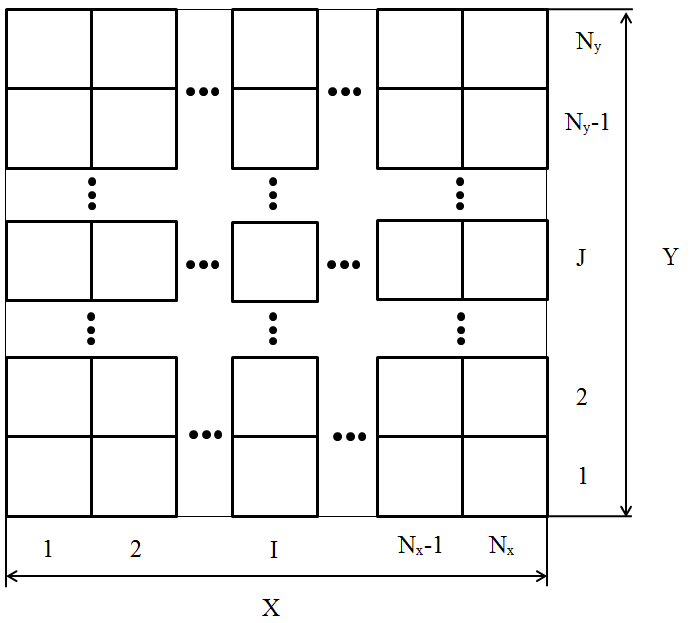
\includegraphics[width=0.60\textwidth]{figures/sec_DSA/fourier_sq_layout.png}
\caption[Fourier domain]{Fourier domain for 2D quadrilateral cells or an axial slice of 3D hexahedral cells in a regular grid.}
\label{fig::DSA_fourier_grid_layout}
\end{figure}

\begin{figure}
\centering
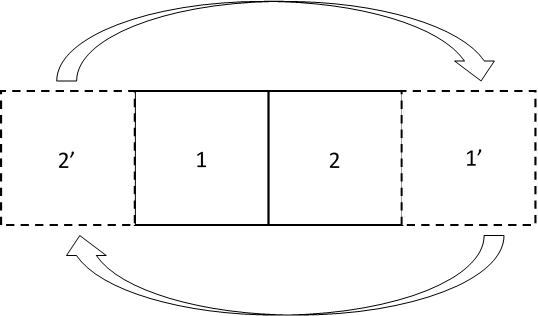
\includegraphics[width=0.65\textwidth]{figures/sec_DSA/Fourier_periodic_BC.png}
\caption[Fourier periodic boundary conditions]{Representation of the periodic boundary conditions used for Fourier analysis for a 2-cell geometric layout.}
\label{fig::DSA_fourier_periodic_BC}
\end{figure}

Once the geometric domain is specified, we can then expand the solution vectors in terms of the domain's Fourier modes. The wave numbers of the Fourier modes, $\vec{\lambda}$, span the interval $[0,\frac{2 \pi}{X}) \otimes [0,\frac{2 \pi}{Y})$ in 2D and $[0,\frac{2 \pi}{X}) \otimes [0,\frac{2 \pi}{Y})\otimes [0,\frac{2 \pi}{Z})$ in 3D. The wave numbers have the definition of $\vec{\lambda} = [\lambda_x, \lambda_y]$ in 2D and $\vec{\lambda} = [\lambda_x, \lambda_y, \lambda_z]$ in 3D. Given a particular wave number, $\vec{\lambda}$, the error modes for the angular flux can be given by the following Fourier ansatz,

\begin{equation}
\label{eq::fourier_ang_sol}
\Psi^{(k)}  (\vec{r}, \vec{\Omega})=  \hat{\Psi}^{(k)} (\vec{\Omega}) \, e^{i \vec{\lambda} \cdot \vec{r}},
\end{equation}

\noindent where $i=\sqrt{-1}$ and $\hat{\Psi}^{(k)} (\vec{\Omega})$ is the Fourier expansion coefficient for the angular flux.  Also, the error modes for the discretized angular flux along direction $m$ and the flux moments can be given by

\begin{equation}
\label{eq::fourier_ang_sol_disc}
\Psi_m^{(k)}  (\vec{r})=  \hat{\Psi}_m^{(k)}  \, e^{i \vec{\lambda} \cdot \vec{r}},
\end{equation}

and

\begin{equation}
\label{eq::fourier_phi_sol}
\Phi^{(k)} (\vec{r}) = \hat{\Phi}^{(k)} e^{i \vec{\lambda} \cdot \vec{r}},
\end{equation}

\noindent respectively. In Eqs. (\ref{eq::fourier_ang_sol}) - (\ref{eq::fourier_phi_sol}), we see that the term $e^{i \vec{\lambda} \cdot \vec{r}}$ acts to transform the spatial parameter into the complex space. For a collection of error modes ({\em e.g.,} the degrees of freedom of a mesh cell) corresponding to the spatial locations ($\vec{r}_1,\vec{r}_2,\vec{r}_3,\vec{r}_4$), we can express Eq. (\ref{eq::fourier_phi_sol}) by

\begin{equation}
\label{eq::fourier_phi_apply_phase}
\Phi^{(k)} (\vec{r}) = \mathbb{P} (\vec{\lambda})   \hat{\Phi}^{(k)} ,
\end{equation}

\noindent where the diagonal phase matrix has the form:

\begin{equation}
\label{eq::fourier_phase_matrix}
\mathbb{P} (\vec{\lambda}) = \left[
\begin{array}{cccc}
e^{i \vec{\lambda} \cdot \vec{r}_1} & 0 & 0 & 0\\
0 & e^{i \vec{\lambda} \cdot \vec{r}_2} & 0 & 0 \\
0 & 0 & e^{i \vec{\lambda} \cdot \vec{r}_3} & 0 \\
0 & 0 & 0 & e^{i \vec{\lambda} \cdot \vec{r}_4} 
\end{array}
\right] \, .
\end{equation}

\noindent One can also utilize an alternative version of Eq. (\ref{eq::fourier_phase_matrix}) by using exponent laws and physical offsets ($\Delta x, \Delta y$) from some starting base point.

Now that we have defined our periodic heterogeneous domain configuration and expressed the expansion of the flux solutions in terms of their Fourier modes, we can now detail how to compile the FA iteration matrix. Recall from Section \ref{sec::DSA_DSA} the different iteration matrices expressing our accelerated transport iterations. Equations (\ref{eq::DSA_ops_update_new}), (\ref{eq::DSA_TG_op_update_simple}), (\ref{eq::DSA_MTG_op_update_simple}), and (\ref{eq::DSA_WGS_op_update_simple}) give the accelerated transport iteration matrices for the 1-group DSA scheme, the Two-Grid scheme, the Modified Two-Grid scheme, and Multigroup Jacobi Acceleration scheme, respectively. Each of these matrices can be expressed in the Fourier phase space by appropriate application of the phase matrices, $\mathbb{P} (\vec{\lambda}) $. For example, let's consider the simple case of the 1-group DSA scheme. The FA iteration matrices for unaccelerated and accelerated Richardson iterations are given by

\begin{equation}
\label{eq::fourier_SI_iter}
{\bf D} \tilde{{\bf L}}^{-1} {\bf M} \tilde{{\bf \Sigma}} ,
\end{equation}

\noindent and

\begin{equation}
\label{eq::fourier_SIDSA_iter}
{\bf D} \tilde{{\bf L}}^{-1} {\bf M} \tilde{{\bf \Sigma}} + {\bf P } \tilde{{\bf A }}^{-1} {\bf X } \tilde{{\bf \Sigma }} \left( {\bf D} \tilde{{\bf L}}^{-1} {\bf M} \tilde{{\bf \Sigma}}  - {\bf I }  \right),
\end{equation}

\noindent respectively. In Eqs. (\ref{eq::fourier_SI_iter}) and (\ref{eq::fourier_SIDSA_iter}), the $\tilde{{\bf L}}$, $\tilde{{\bf \Sigma}}$, and $\tilde{{\bf A}}$ operators have had phase transformations applied, which we denote with the overhead tilde, $\tilde{}$. During the assembly of the transport and diffusion operators, the phase transformations can be applied with the right-multiplication of the appropriate phase matrix on the corresponding elementary matrices. We note that when assembling the face coupling terms on the domain boundary, the base phase of the cell on the other side of the periodic boundary is not used. Instead, the phase corresponding to the virtual cell is used. For example, let us analyze the left face of cell 1 in Figure \ref{fig::DSA_fourier_periodic_BC}. When applying the periodic condition, we use the degrees of freedom corresponding to cell 2, but use the phase matrix corresponding to cell 2'. Finally, we note that the FA iteration matrices for the thermal neutron upscattering acceleration methods are computed in an identical manner.

Once the FA iteration matrix is assembled for a given wave number, $\vec{\lambda}$, we compute all of its corresponding eigenvalues. The largest of these eigenvalues is the spectral radius for the given wave number. If we compute the spectral radii for all the possible wave numbers ({\em e.g.,} $[0,\frac{2 \pi}{X}) \otimes [0,\frac{2 \pi}{Y})$ in 2D) for a given problem configuration, then the maximum corresponds to the global spectral radius for the problem. For Richardson iteration in the asymptotic regime, we will converge to our transport solution more rapidly with a smaller spectral radius that is strictly less than 1. Likewise, our scheme would be unstable if the spectral radius is larger than 1. 

For this work, all Fourier analysis was performed in MATLAB. All the eigenmodes corresponding to a Fourier wave number for a given iteration matrix can be easily computed with MATLAB's built-in {\em eig} function. The maximum eigenvalue is found over the wave number space by use of the Nelder-Mead simplex algorithm \cite{nelder1965simplex}. We stress that some sort of minimization algorithm must be employed because some problem configurations can have extremely narrow local maxima. These difficult-to-find local maxima can correspond to the global maximum which is our desired spectral radius that we wish to compute. 

We illustrate the necessity for a minimization algorithm in Figure \ref{fig::DSA_fourier_modes_showing_search_need}. We have modeled a single 2D square mesh cell with dimensions $X=1$ and $Y=1$. The total cross section, $\sigma_t$, is set to $10^{-2}$ and the scattering ratio, $c$, set to 0.9999. We use the $S4$ level-symmetric quadrature set. The left image of Figure \ref{fig::DSA_fourier_modes_showing_search_need} has the 2D Fourier wave number span the full domain space of $[\lambda_x,\lambda_y]=[0,2 \pi]^2$. The right image zooms in on the wave number ranging: $[\lambda_x,\lambda_y]=[0,1/4]^2$. From the right image, we can see two extremely narrow local maxima. We can qualitatively ascertain that these local maxima would be difficult to find if we had simply laid a grid of wave number points over $[0,2 \pi]^2$. It would require a very fine wave number grid that is both expensive to compute and not guaranteed to locate the maximum. Chang and Adams presented an even more extreme example of a difficult to find global maximum using transport synthetic acceleration \cite{chang2003analysis}.

\begin{figure}
\centering
	\begin{subfigure}[b]{0.48\textwidth}
		\centering
		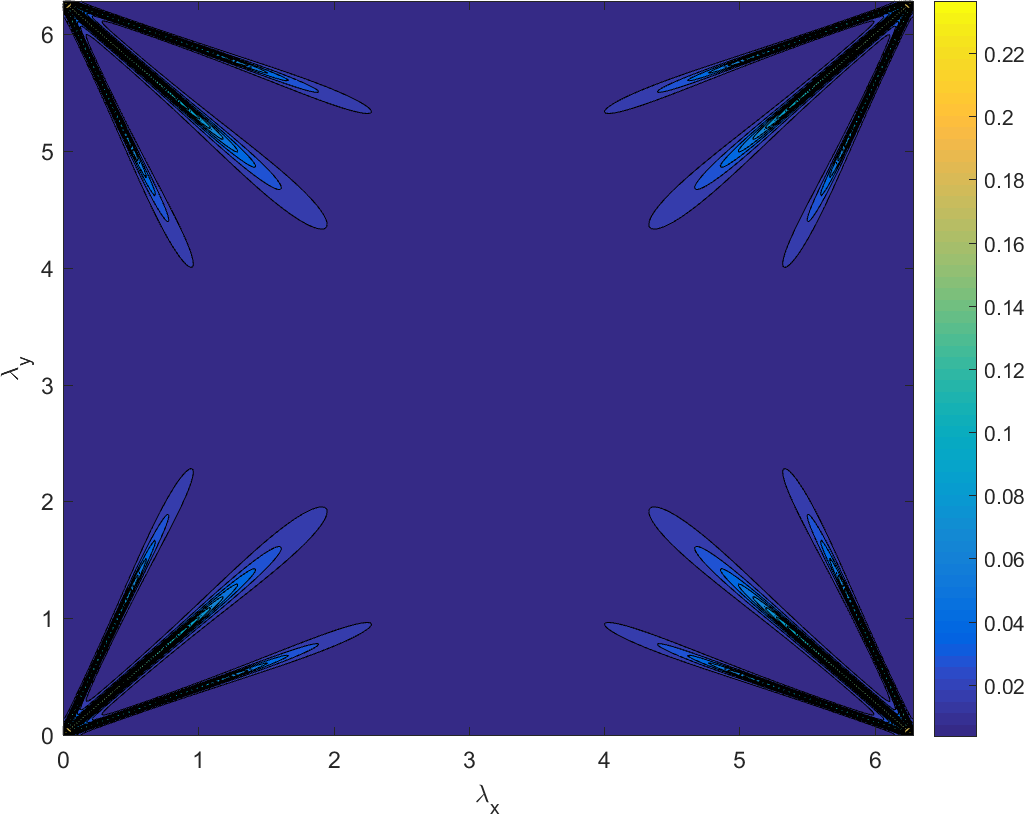
\includegraphics[width=\textwidth]{figures/sec_DSA/SI_MIP_C=4_UPWLD1_LS4_x=1e-2_dydx=1_contour.png}
		\caption{}
	\end{subfigure}
	\hfill
	\begin{subfigure}[b]{0.495\textwidth}
		\centering
		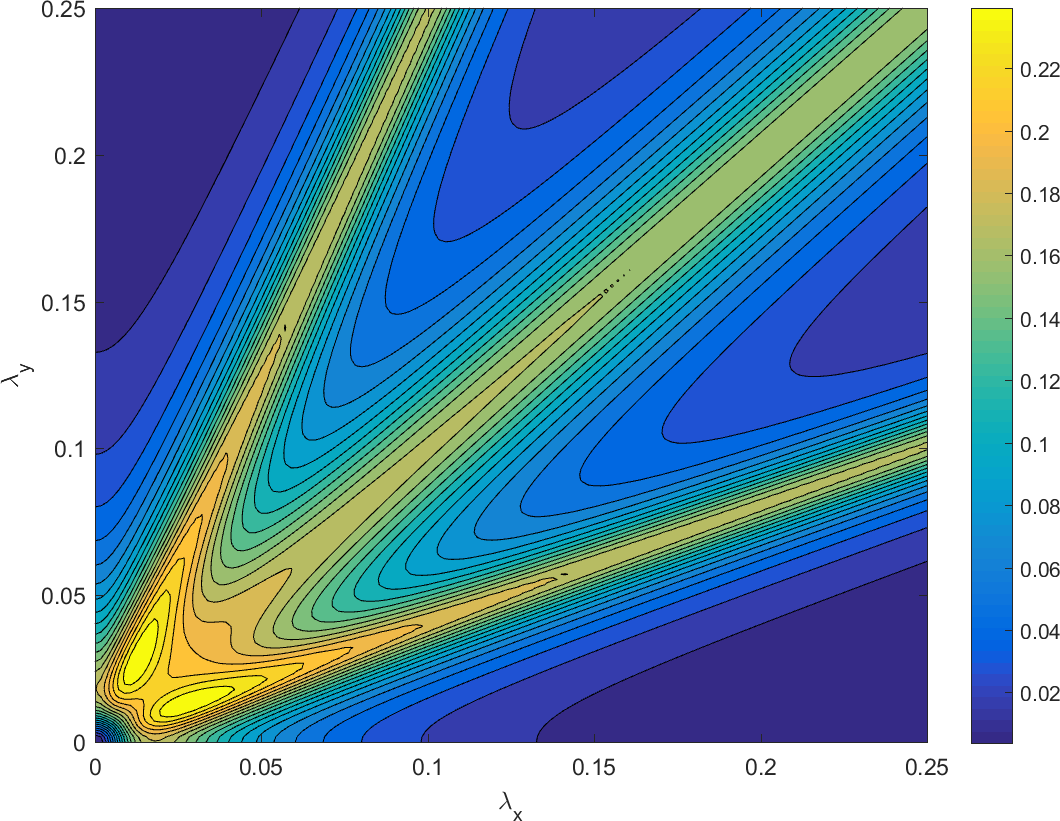
\includegraphics[width=\textwidth]{figures/sec_DSA/SI_MIP_C=4_UPWLD1_LS4_x=1e-2_dydx=1_contour_ZOOM.png}
		\caption{}
	\end{subfigure}
\caption[2D Fourier wave form for MIP with the PWL coordinates]{2D Fourier wave form for MIP, with 1 square cell with 1e-2 mfp, with the PWL coordinates, with the LS4 quadrature, and where the wave numbers range from: (a) $[\lambda_x,\lambda_y]=[0,2 \pi]^2$ and (b) $[\lambda_x,\lambda_y]=[0,1/4]^2$.}
\label{fig::DSA_fourier_modes_showing_search_need}
\end{figure}

%%%%%%%%%%%%%%%%%%%%%%%%%%%%%%%%%%%%%%%%%%%%%%%%%%%
%%%%%%%%%%%%%%%%%%%%%%%%%%%%%%%%%%%%%%%%%%%%%%%%%%%
%%%   Section - Results
%%%%%%%%%%%%%%%%%%%%%%%%%%%%%%%%%%%%%%%%%%%%%%%%%%%
%%%%%%%%%%%%%%%%%%%%%%%%%%%%%%%%%%%%%%%%%%%%%%%%%%%
\section{Numerical Results}
\label{sec::DSA_Results}

We now present all theoretical and applied results pertaining to the described DSA schemes. First, we provide results in Section \ref{sec::DSA_Results_SIP} on the efficacy of the SIP form as a diffusion solver. Section \ref{sec::DSA_Results_1G} provides all theoretical and numerical results pertaining the 1-group DSA scheme. Then, Section \ref{sec::DSA_Results_Scaling} demonstrates the scalability of the MIP diffusion form on massively-parallel computer architectures. Finally, Section \ref{sec::DSA_Results_IM1} gives the results pertaining to the analysis performed for the thermal neutron upscattering acceleration methods.

%%%%%%%%%%%%%%%%%%%%%%%%%%%%%%%%%%%%%%%%%%%%%%%%%%%
%%%   SubSection - SIP Results
\subsection{SIP used as a Diffusion Solver}
\label{sec::DSA_Results_SIP}

We first wish to know how an interior penalty form of the diffusion equation will perform on unstructured polyhedral grids. The SIP diffusion formulation has previously been analyzed for use as a DFEM diffusion solver for unstructured 2D polygonal grids \cite{ragusa2015discontinuous}. The MIP DSA form has also been successfully utilized for unstructured 2D polygonal grids \cite{turcksin2014discontinuous}. Here, we first seek to extend the efficacy of the SIP form as a diffusion solver on polyhedral mesh cellls. We will do this by analyzing the following two problem types:

\begin{enumerate}
	\item An exactly-linear solution to determine if linear basis functions will span the solution space;
	\item The Method of Manufactured Solutions (MMS) to test basis function convergence rates.
\end{enumerate}

The polyhedral mesh types that we employ for this analysis are presented in Section \ref{sec::DSA_Results_SIP_Geometry}. Next, the exactly-linear solution analysis is performed in Section \ref{sec::DSA_Results_SIP_Linear}. Finally, the MMS analysis to confirm the second order convergence rates of the 3D PWL basis functions is presented in Section \ref{sec::DSA_Results_SIP_MMS}.

%%%%%%%%%%%%%%%%%%%%%%%%%%%%%%%%%%%%%%%%%%%%%%%%%%%
%%%   SubSubSection - SIP Results = Geometry
\subsubsection{Geometry Specification for the SIP Problems}
\label{sec::DSA_Results_SIP_Geometry}

To analyze the SIP diffusion form on 3D polyhedral grids, we will utilize many of the 2D polygonal grids that were used for previous analysis in Chapter \ref{sec::BF}. For this analysis we will resuse the cartesian, ordered-triangular, polygonal sinusoidal, and polygonal-z meshes. We will also use purely-randomized polygonal grids formed from Voronoi mesh generation as outlined in Section \ref{sec::Sn_Solution_Spatial_Voronoi}. To form the needed 3D polyhedral grids, we will take these 2D grids and simply extrude the meshes in the z-dimension. 

Figure \ref{fig::SIP_mesh_slices} provides the 2D mesh types that will be utilized in this analysis. Figure \ref{fig::SIP_mesh_extruded} then provides the same meshes after they have been extruded in the z-dimension. We note that it will not simply be these exact grids that are employed. For the MMS analysis in Section \ref{sec::DSA_Results_SIP_MMS}, various refinements of these meshes will be utilized.

\begin{figure}
\centering
	\begin{subfigure}[b]{0.5\textwidth}
		\centering
		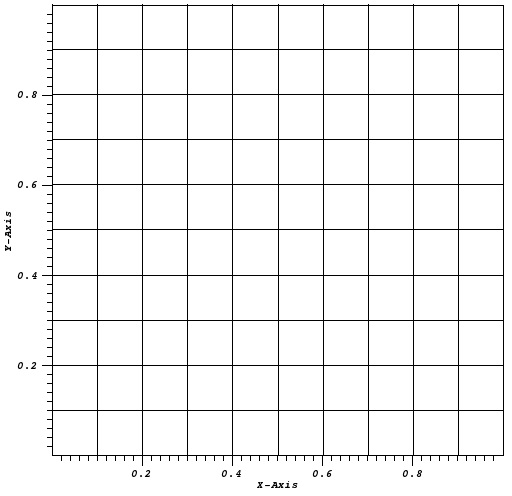
\includegraphics[width=0.82\textwidth]{figures/sec_DSA/SIP_cart_mesh.png}
		\caption{Cartesian}
	\end{subfigure}
	\vfill
	\begin{subfigure}[b]{0.45\textwidth}
		\centering
		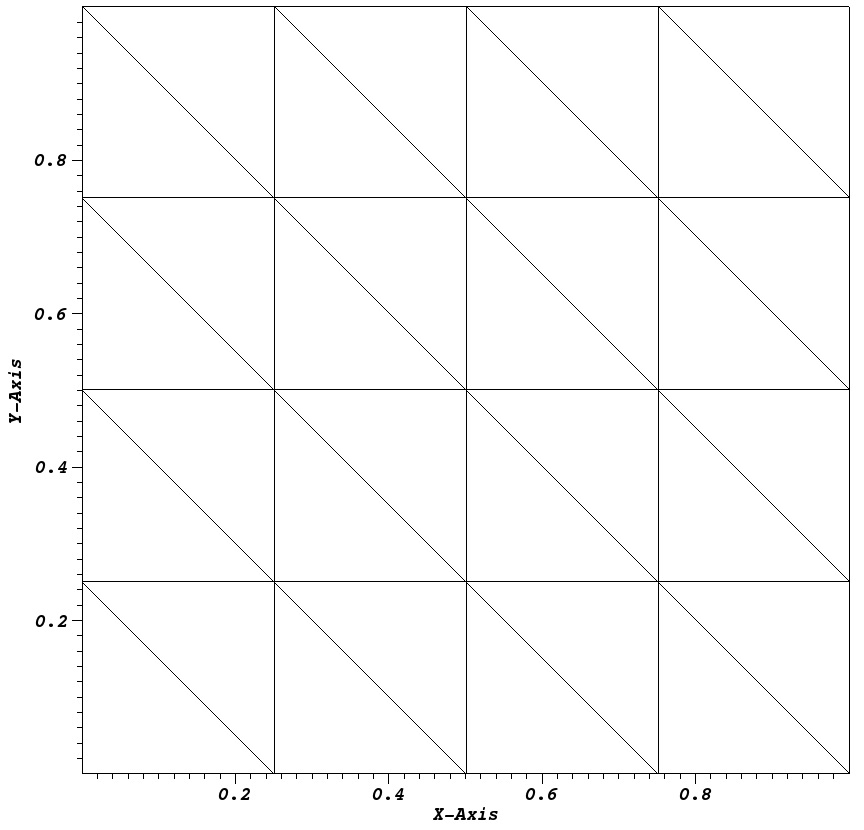
\includegraphics[width=0.85\textwidth]{figures/sec_DSA/SIP_tri_mesh.png}
		\caption{Triangular}
	\end{subfigure}
	\hfill
	\begin{subfigure}[b]{0.45\textwidth}
		\centering
		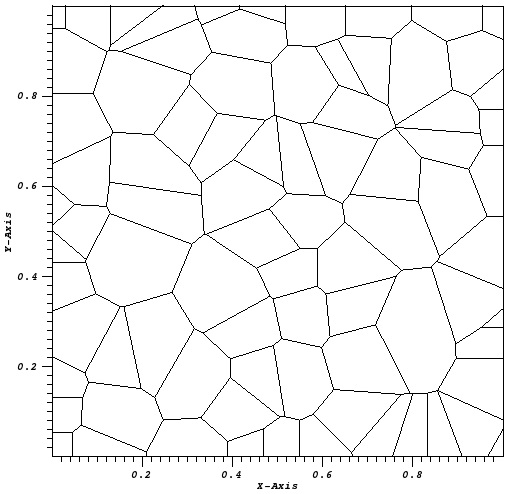
\includegraphics[width=0.85\textwidth]{figures/sec_DSA/SIP_poly_mesh.png}
		\caption{Random Polygons}
	\end{subfigure}
	\vfill
	\begin{subfigure}[b]{0.45\textwidth}
		\centering
		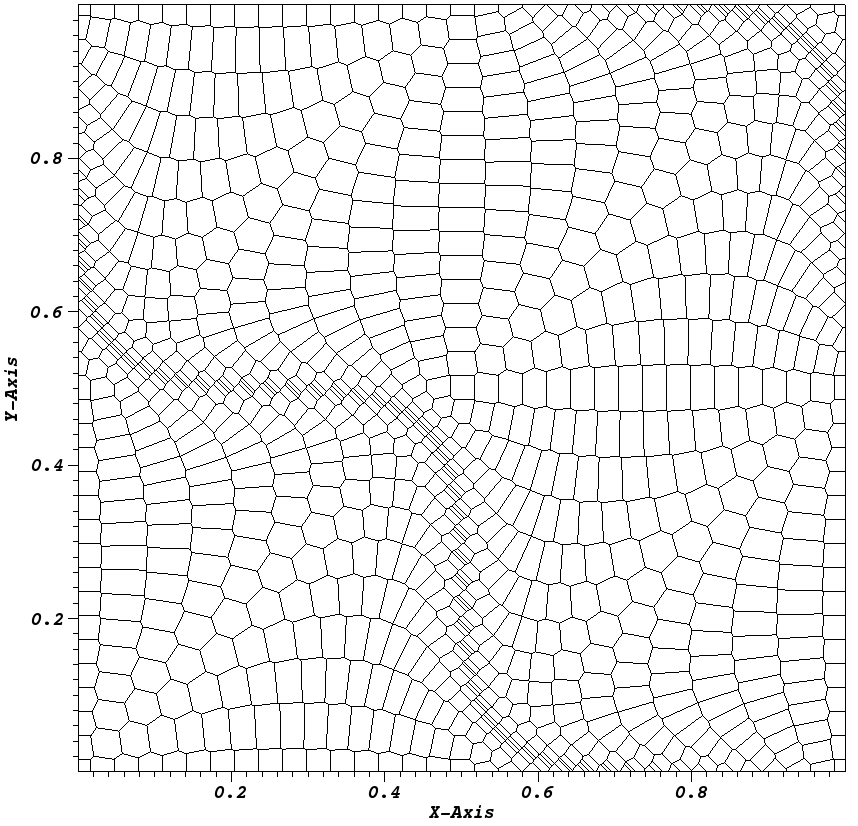
\includegraphics[width=0.85\textwidth]{figures/sec_DSA/SIP_sine_poly_mesh.png}
		\caption{Sinusoid Polygons}
	\end{subfigure}
	\hfill
	\begin{subfigure}[b]{0.45\textwidth}
		\centering
		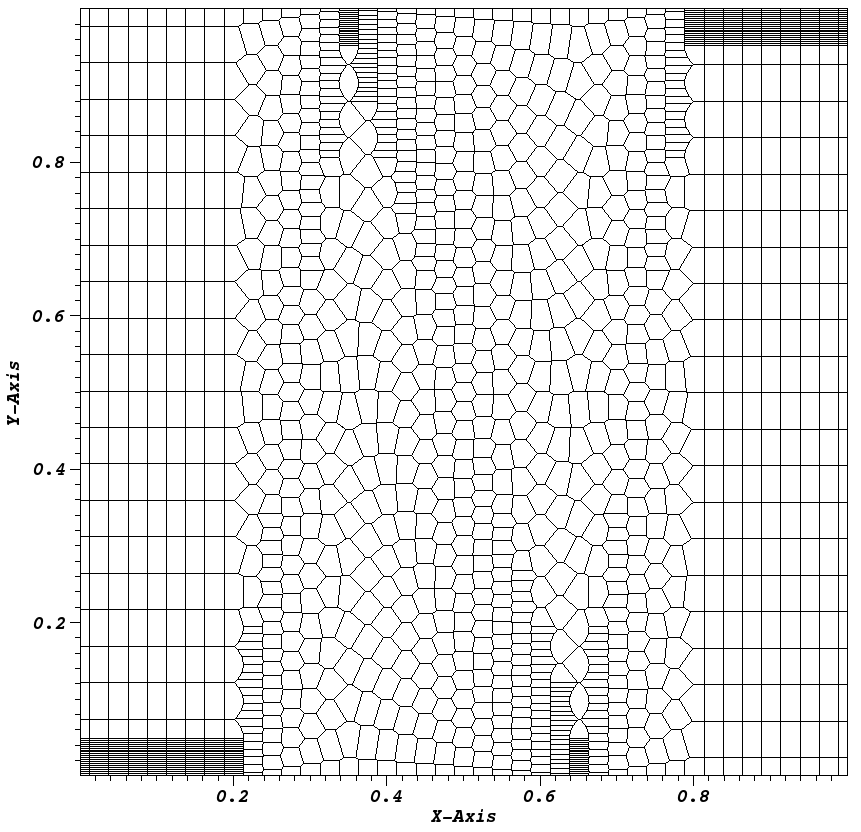
\includegraphics[width=0.85\textwidth]{figures/sec_DSA/SIP_z_poly_mesh.png}
		\caption{Polygonal Z-Mesh}
	\end{subfigure}
\caption{2D polygonal grids to be extruded for the 3D SIP calculations.}
\label{fig::SIP_mesh_slices}
\end{figure}

\begin{figure}
\centering
	\begin{subfigure}[b]{0.5\textwidth}
		\centering
		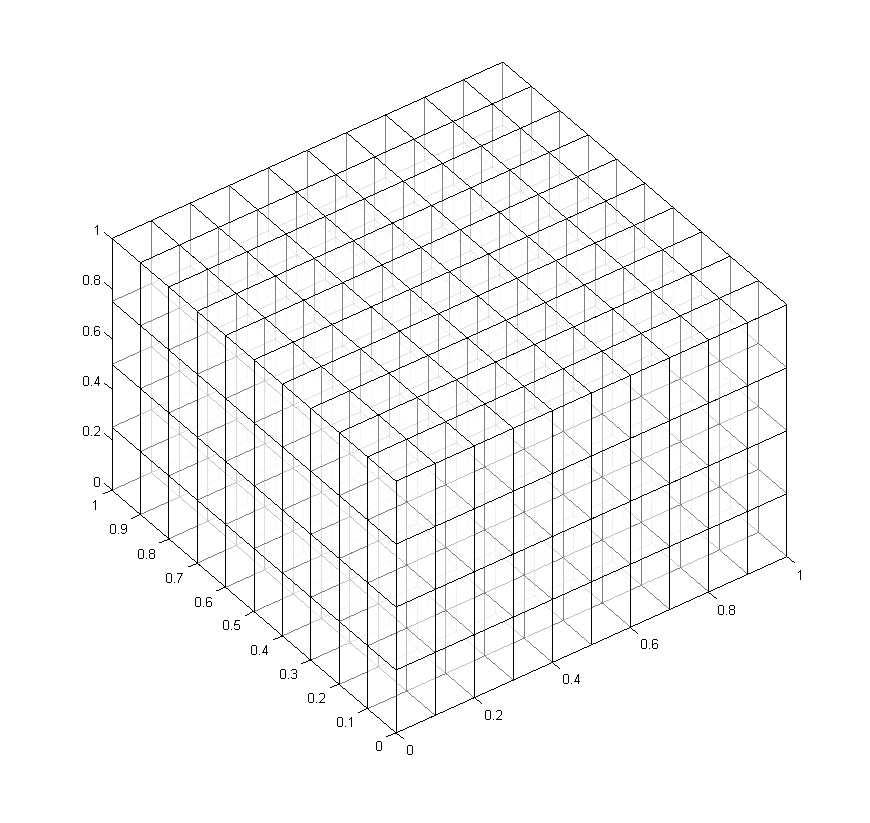
\includegraphics[width=0.82\textwidth]{figures/sec_DSA/SIP_cart_extruded_mesh.png}
		\caption{Cartesian}
	\end{subfigure}
	\vfill
	\begin{subfigure}[b]{0.45\textwidth}
		\centering
		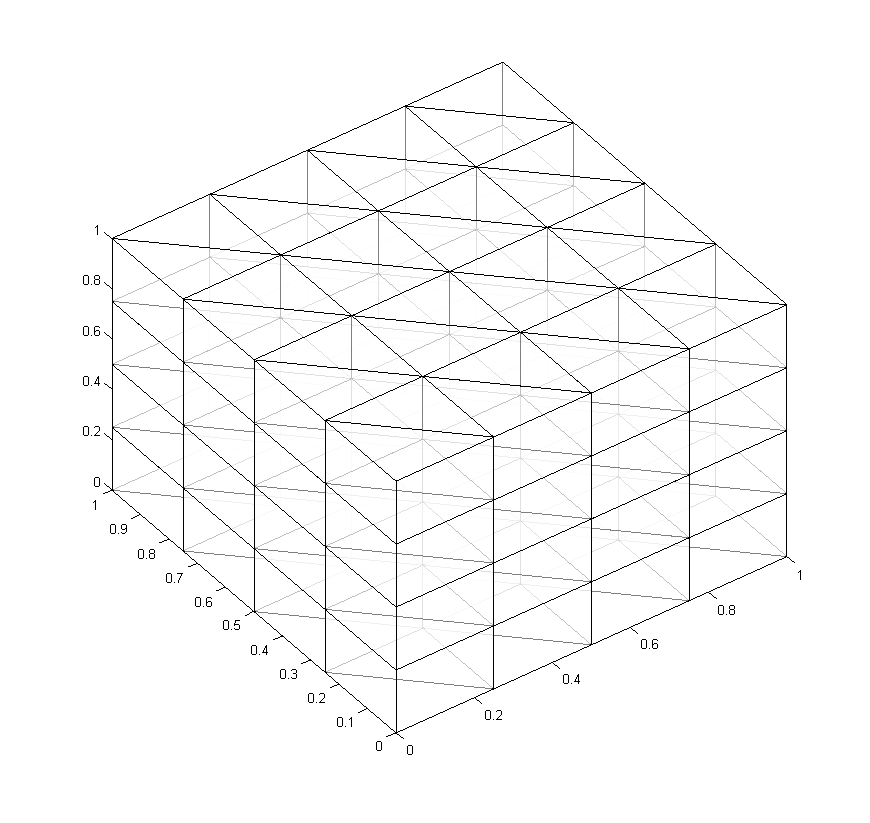
\includegraphics[width=0.85\textwidth]{figures/sec_DSA/SIP_tri_extruded_mesh.png}
		\caption{Triangular}
	\end{subfigure}
	\hfill
	\begin{subfigure}[b]{0.45\textwidth}
		\centering
		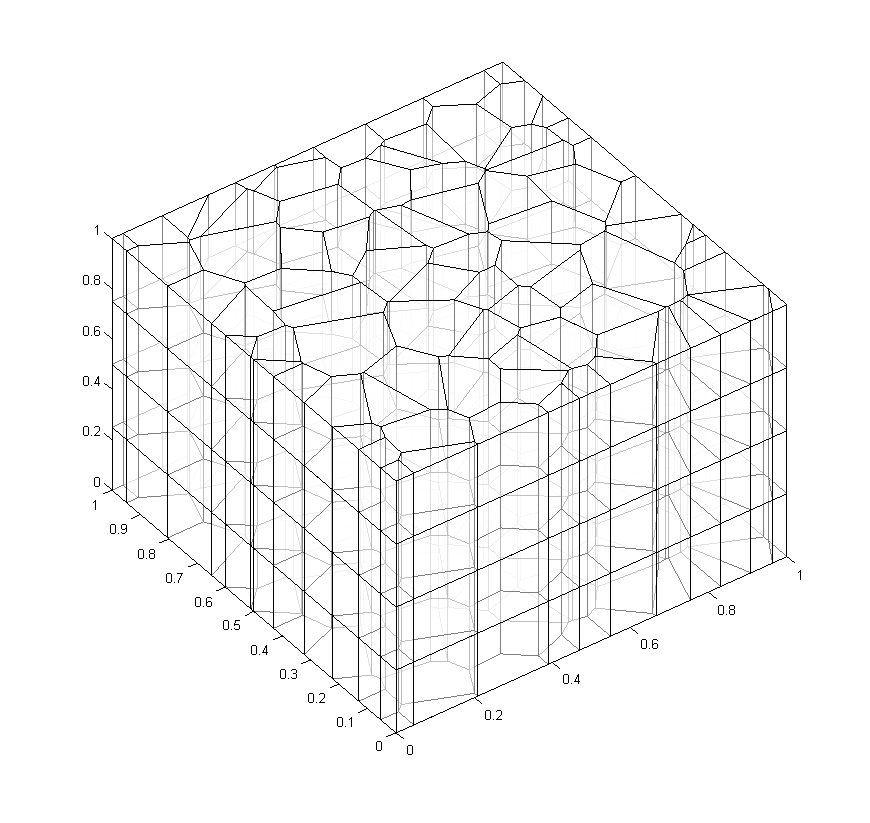
\includegraphics[width=0.85\textwidth]{figures/sec_DSA/SIP_poly_extruded_mesh.png}
		\caption{Random Polygons}
	\end{subfigure}
	\vfill
	\begin{subfigure}[b]{0.45\textwidth}
		\centering
		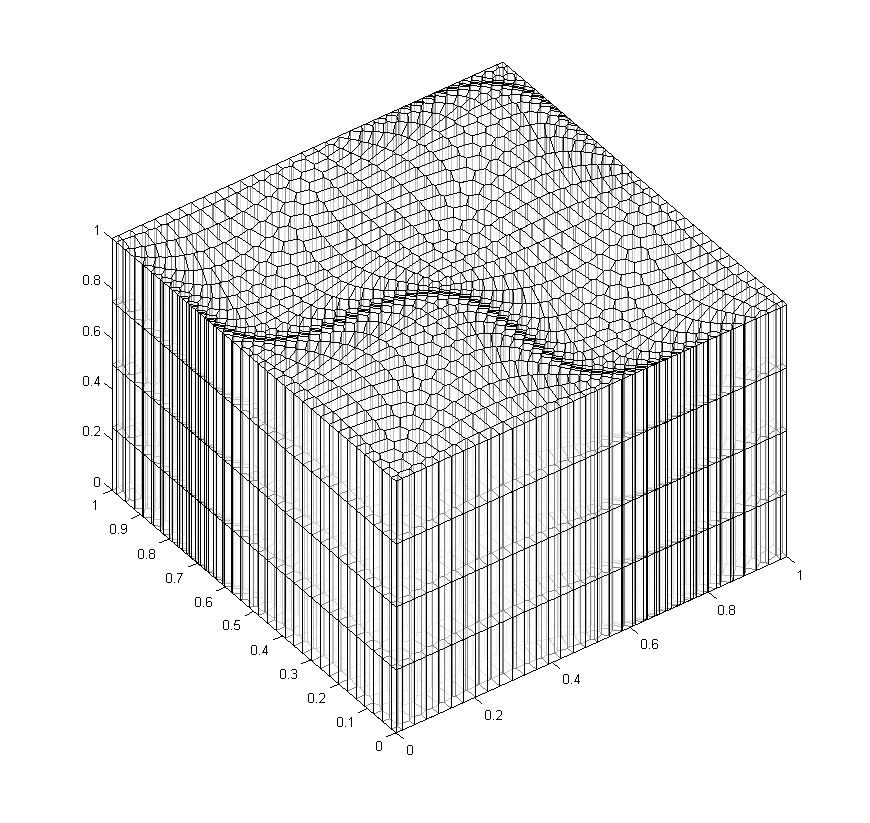
\includegraphics[width=0.85\textwidth]{figures/sec_DSA/SIP_sine_poly_extruded_mesh.png}
		\caption{Sinusoid Polygons}
	\end{subfigure}
	\hfill
	\begin{subfigure}[b]{0.45\textwidth}
		\centering
		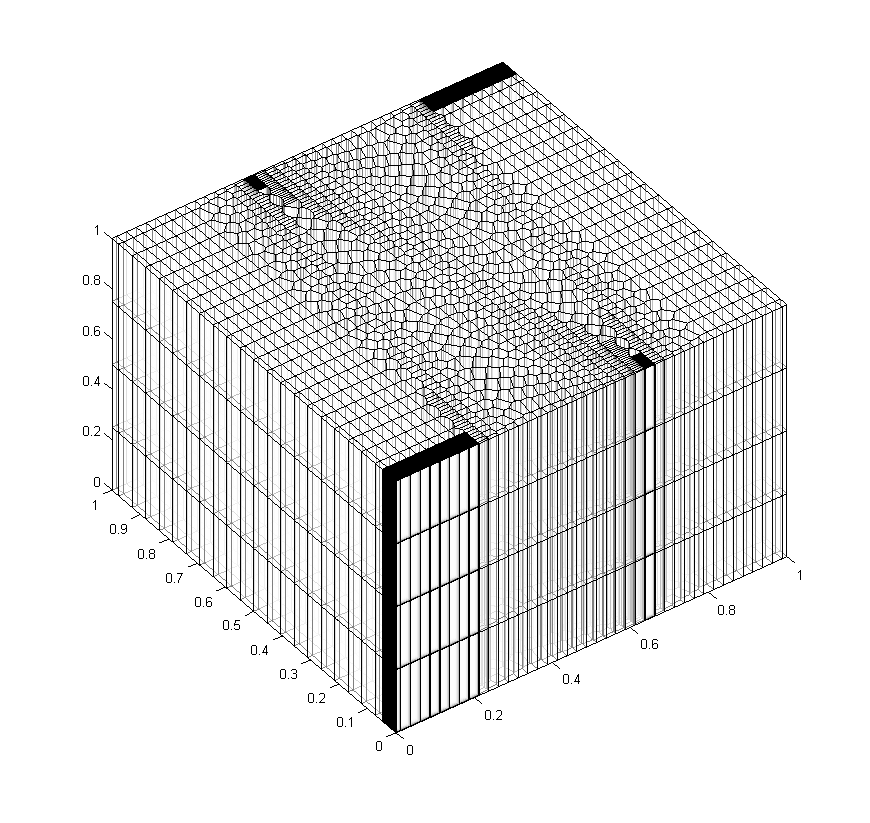
\includegraphics[width=0.85\textwidth]{figures/sec_DSA/SIP_z_poly_extruded_mesh.png}
		\caption{Polygonal Z-Mesh}
	\end{subfigure}
\caption{Extrusion of the different polygonal meshes.}
\label{fig::SIP_mesh_extruded}
\end{figure}

%%%%%%%%%%%%%%%%%%%%%%%%%%%%%%%%%%%%%%%%%%%%%%%%%%%
%%%   SubSubSection - SIP Results = Linear
\subsubsection{Exactly-Linear Solution}
\label{sec::DSA_Results_SIP_Linear}

We first test SIP by enforcing a sytem that yields an exactly-linear diffusion solution. Linear finite elements should then theoretically fully-span the solution space. We can achieve this mathematically by setting the cross-section and right-hand-source terms to zero, $\sigma = Q = 0$. Robin boundary conditions are imposed on opposite faces in 1 dimension, with homogeneous Neumann boundary conditions on all other faces. If the Robin boundaries are chosen in the y-direction, with $y \in (0,L)$, then the analytical solution for the problem will be 

\begin{equation}
\label{eq::SIP_mms_lin_solution}
\Phi(x,y,z) = \frac{4 J^{inc}}{L + 4D} \left(  L + 2 D - y \right),
\end{equation}

\noindent with the following boundary conditions in the y-direction:

\begin{equation}
\label{eq::SIP_mms_lin_bcs}
\begin{aligned}
\Phi - 2D \partial_y \Phi = & 4 J^{inc}, \qquad & \forall (x,z),y=0 \\
\Phi + 2D \partial_y \Phi = & 0, \qquad & \forall (x,z),y=L
\end{aligned}.
\end{equation}

\noindent In Eqs. (\ref{eq::SIP_mms_lin_solution}) and (\ref{eq::SIP_mms_lin_bcs}), $D$ is once again the standard diffusion coefficient and $J^{inc}$ is the incoming current on the $y=0$ boundary. For this analysis, we choose $D$ to be 2, $J^{inc}$ to be 9, and $L$ to be 1. Using Eq. (\ref{eq::SIP_mms_lin_solution}), our solution has a value of 20 at $y=0$ and linearly-decreases to 16 at $y=1$.

Using the 3D PWL basis functions, which were previously used for SIP on 2D polygons \cite{ragusa2015discontinuous}, the linear solutions are presented in Figure \ref{fig::SIP_linear_sol} at the midplane axial slice of $z=L/2$. We can see from the exact contour lines in the plots that SIP can capture an exactly-linear solution even on some highly distorted polyhedral grids.

\begin{figure}
\centering
	\begin{subfigure}[b]{0.5\textwidth}
		\centering
		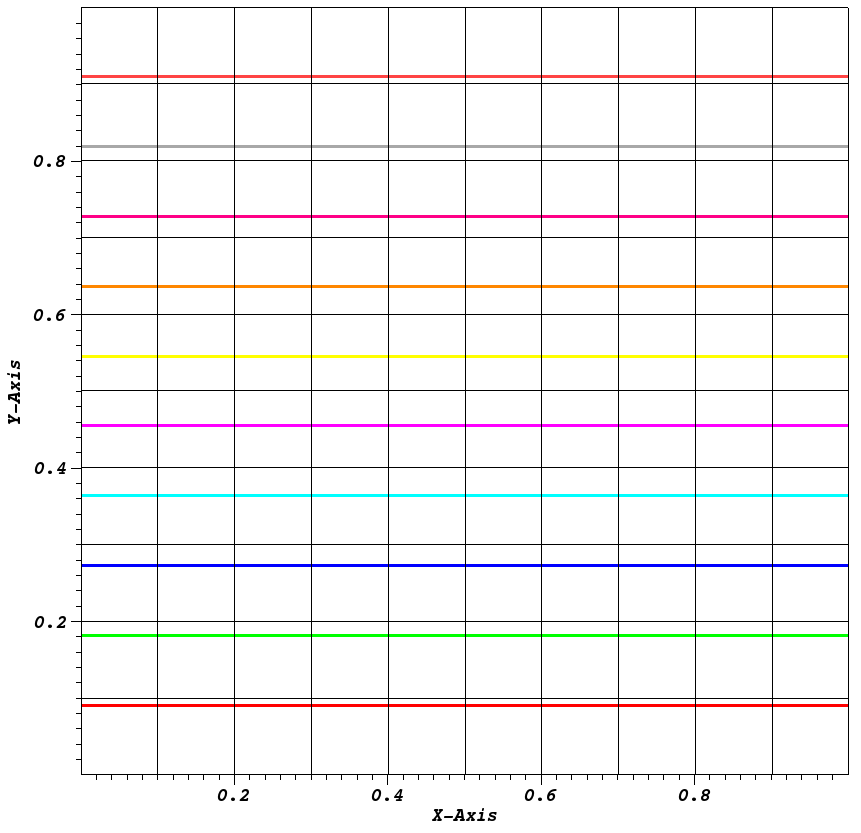
\includegraphics[width=0.82\textwidth]{figures/sec_DSA/SIP_cart_lin_contour.png}
		\caption{Cartesian}
	\end{subfigure}
	\vfill
	\begin{subfigure}[b]{0.45\textwidth}
		\centering
		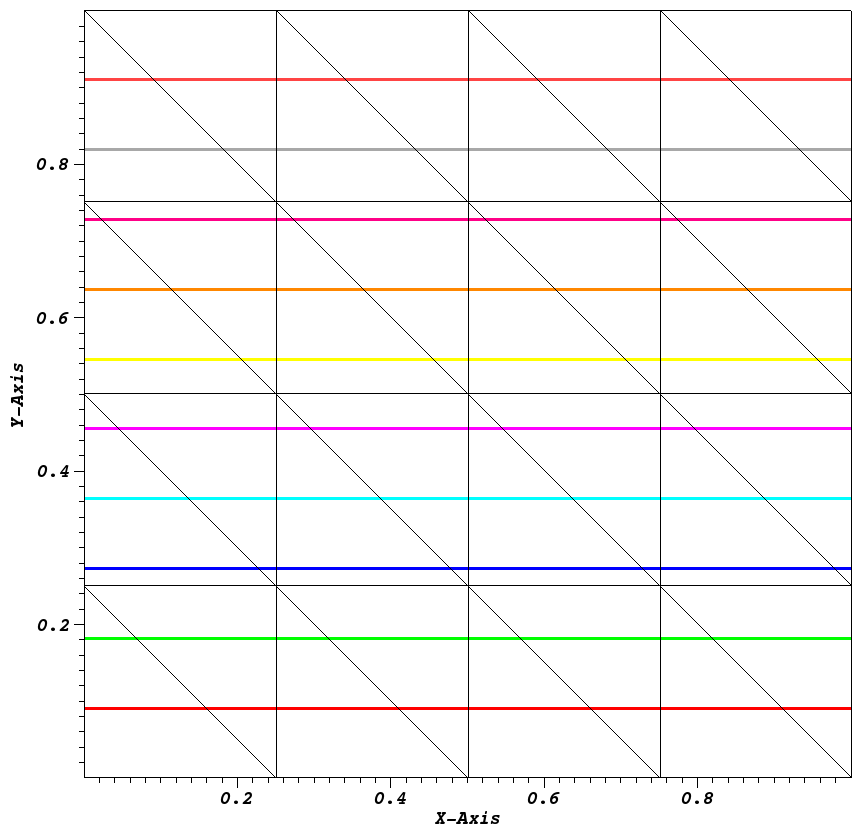
\includegraphics[width=0.85\textwidth]{figures/sec_DSA/SIP_tri_lin_contour.png}
		\caption{Triangular}
	\end{subfigure}
	\hfill
	\begin{subfigure}[b]{0.45\textwidth}
		\centering
		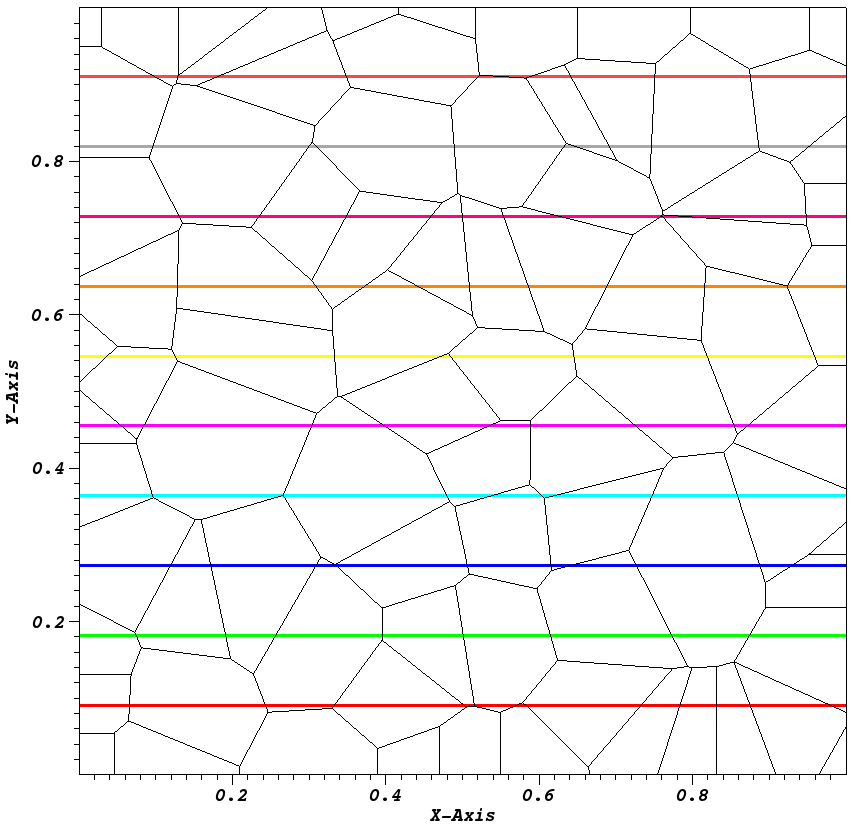
\includegraphics[width=0.85\textwidth]{figures/sec_DSA/SIP_poly_lin_contour.png}
		\caption{Random Polygons}
	\end{subfigure}
	\vfill
	\begin{subfigure}[b]{0.45\textwidth}
		\centering
		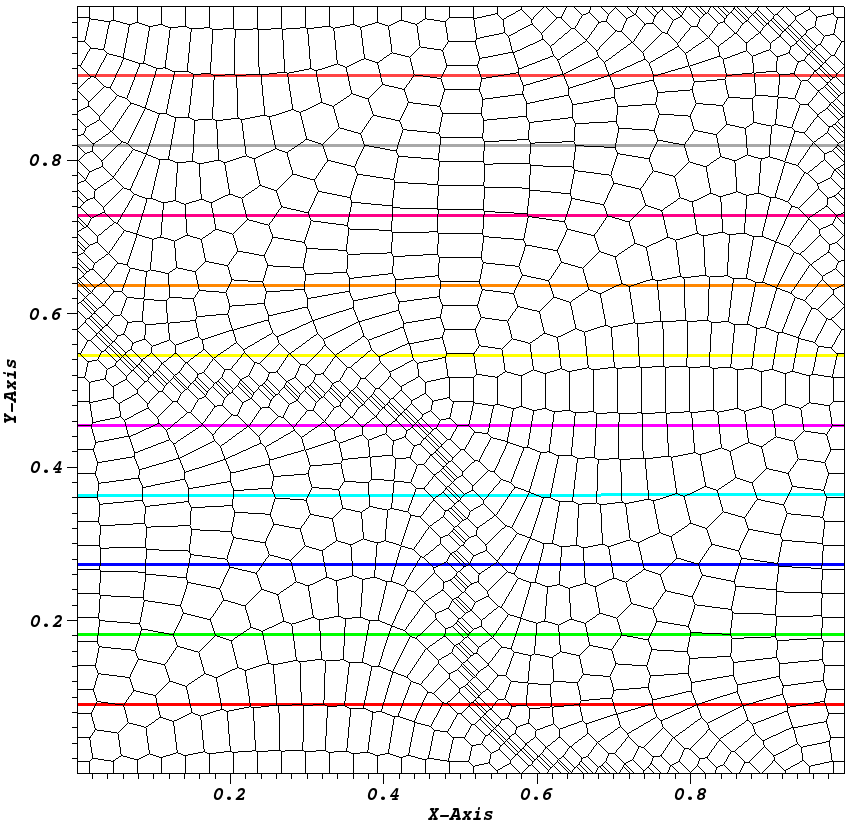
\includegraphics[width=0.85\textwidth]{figures/sec_DSA/SIP_sine_poly_lin_contour.png}
		\caption{Sinusoid Polygons}
	\end{subfigure}
	\hfill
	\begin{subfigure}[b]{0.45\textwidth}
		\centering
		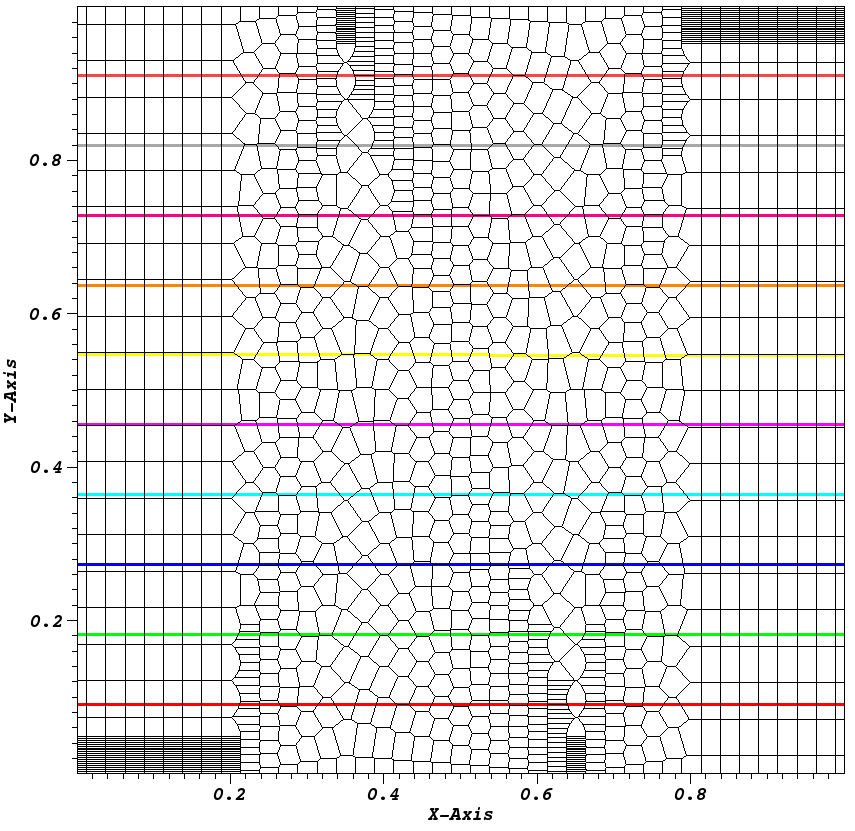
\includegraphics[width=0.85\textwidth]{figures/sec_DSA/SIP_z_poly_lin_contour.png}
		\caption{Polygonal Z-Mesh}
	\end{subfigure}
\caption{Axial slice showing the contours for the linear solution of the SIP diffusion form.}
\label{fig::SIP_linear_sol}
\end{figure}

%%%%%%%%%%%%%%%%%%%%%%%%%%%%%%%%%%%%%%%%%%%%%%%%%%%
%%%   SubSubSection - SIP Results = MMS
\subsubsection{Method of Manufactured Solutions}
\label{sec::DSA_Results_SIP_MMS}

We next test to see if the SIP diffusion form can capture the appropriate second order convergencerates with the 3D PWL basis functions. These basis functions were previously shown to capture the appropriate convergence rates for the DGFEM transport equation on 3D hexahedral grids \cite{bailey2008phd}. The convergence for the SIP diffusion form is similar to the DGFEM transport equation. Since there are no impositions on the regularity of the diffusion solution, then the SIP convergence rate in the $L_2$-norm can be given by

\begin{equation}
\label{eq::SIP_convergence_h}
|| \Phi - \Phi_h ||_{L_2} \leq C h^{p+1}.
\end{equation}

\noindent In a similar manner to the DGFEM transport equation, we can express a proportional relation between the mesh cell diameters, $h$, and the number of degrees of freedom, $N_{dof}$: $N_{dof} \propto h^{-d}$. Therefore, the convergence rate of the SIP diffusion form can be expressed with the degrees of freedom as 

\begin{equation}
\label{eq::SIP_convergence_N}
|| \Phi - \Phi_h ||_{L_2} \leq C N_{dof}^{-\frac{p+1}{d}}.
\end{equation}

\noindent Equation (\ref{eq::SIP_convergence_N}) states that for this 3D problem using linear basis functions, we expect the slope of our convergence rates to be $-2/3$.

We test two different MMS solutions: 1) a pairwise quadratic function and 2) a product of the pairwise quadratic function and a localized Gaussian function. The quadratic and Gaussian functions are given by 

\begin{equation}
\label{eq::SIP_quad_mms_solution}
\begin{aligned}
\Phi^{quad} (x,y,z) = x(1-x)y(1-y)z(1-z) ,
\end{aligned}
\end{equation}

\noindent and

\begin{equation}
\label{eq::SIP_gauss_mms_solution}
\begin{aligned}
\Phi^{gauss} (x,y,z) = \Phi^{quad} (x,y,z) \exp(- (\vec{r} - \vec{r}_0) \cdot (\vec{r} - \vec{r}_0)^{T}  ),
\end{aligned}
\end{equation}

\noindent respectively, where $\vec{r} = (x,y,z)$ and $\vec{r}_0 = (x_0,y_0,z_0)$. We plot the MMS error of the SIP diffusion form in Figure \ref{fig::SIP_mms_error_plot} for both the quadratic and Gaussian solutions. We also provide solutions using a CFEM diffusion form for comparison. In Figure \ref{fig::SIP_mms_error_plot}, we clearly see that SIP captures the proper convergence rate. It is also easy to see that the CFEM diffusion solutions provide reduced error based on the number of spatial degrees of freedom. This is an obvious result since SIP has multiple degrees of freedom for every vertex on the mesh whereas CFEM only has 1. However, we will be using the MIP DSA form as the low-order acceleration operator and not as a stand-alone diffusion solver. Therefore, this observed non-optimal convergence rate (as well as capturing the exactly-linear solution) is required (and satisfied).

\begin{figure}
\centering
{
	\begin{subfigure}[b]{0.95\textwidth}
		\centering
		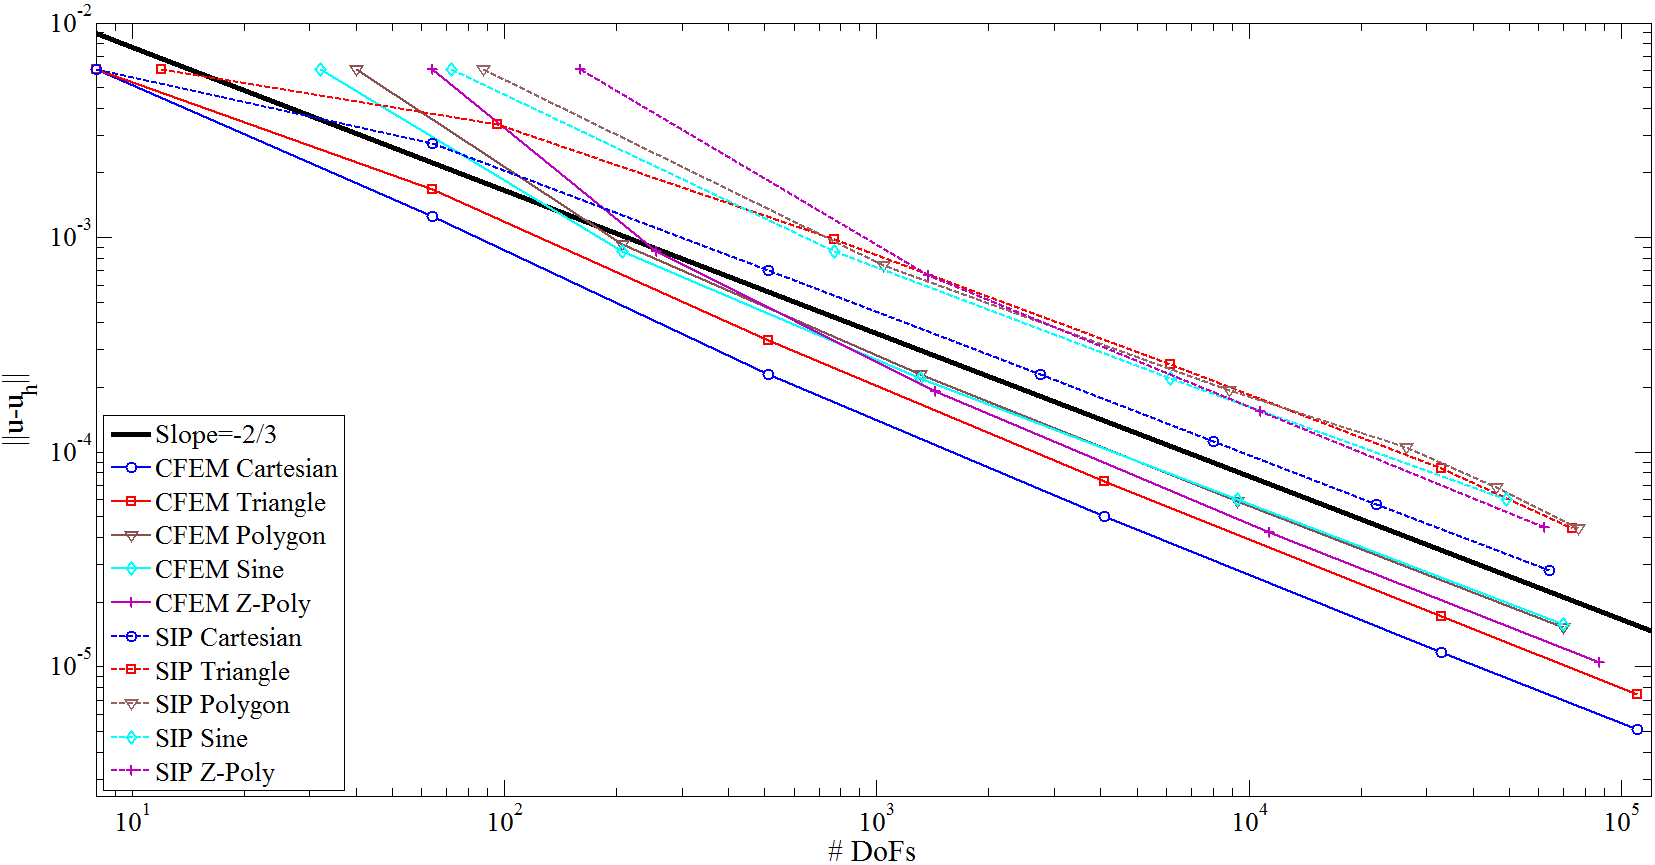
\includegraphics[width=0.95\textwidth]{figures/sec_DSA/SIP_mms_3d_quad_full_paint.png}
		\caption{Quadratic Solution}
	\end{subfigure}
}
\vspace{3mm}
{
	\begin{subfigure}[b]{0.95\textwidth}
		\centering
		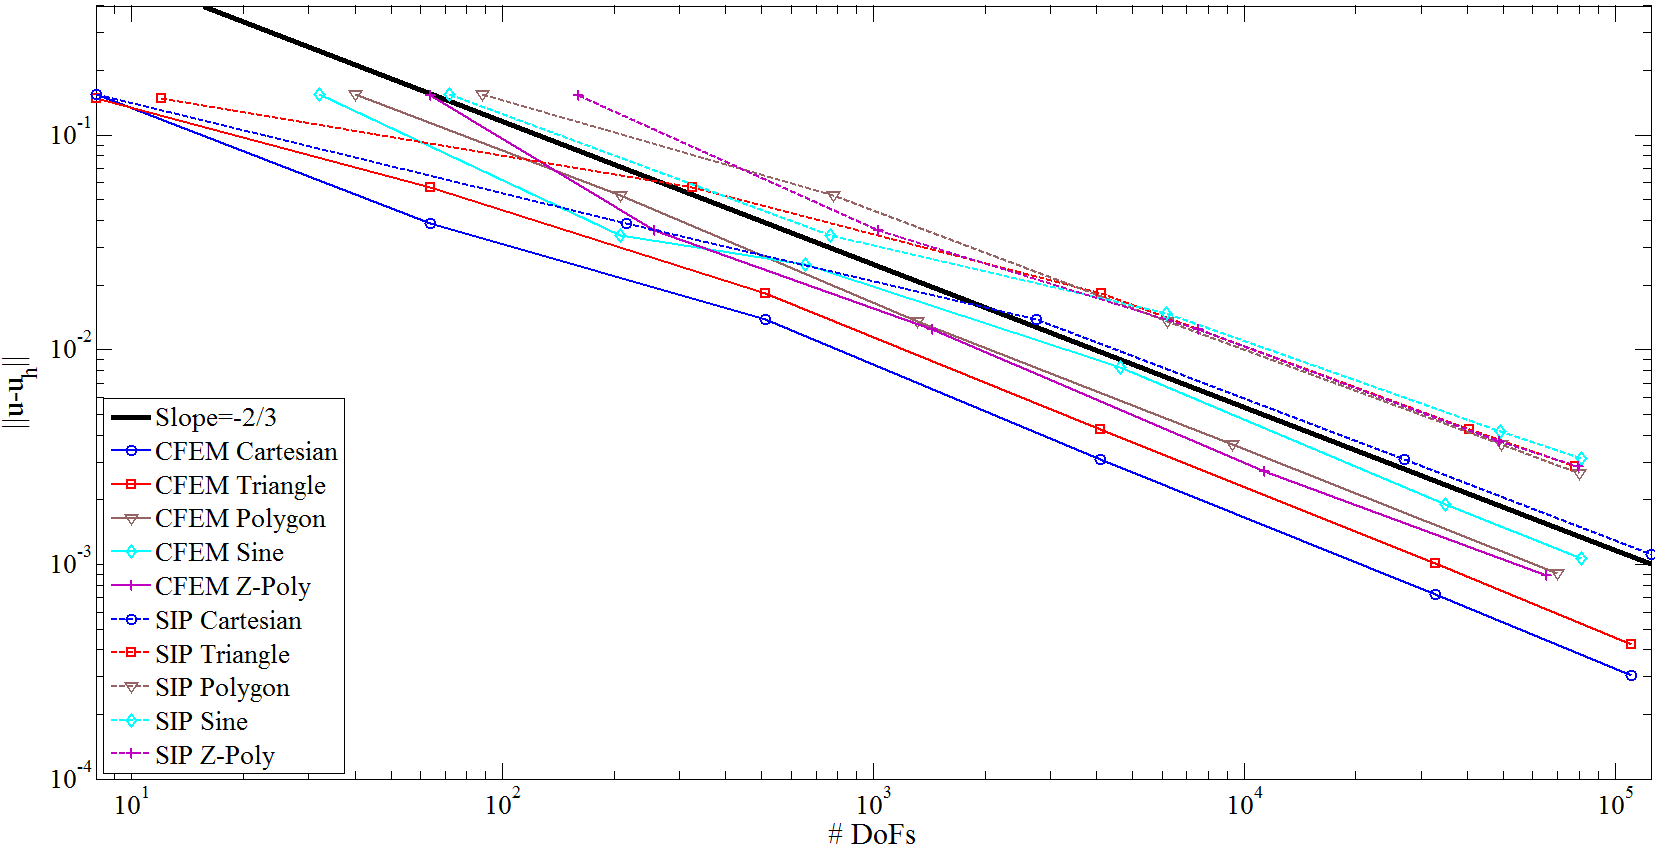
\includegraphics[width=0.95\textwidth]{figures/sec_DSA/SIP_mms_3d_gauss_full_paint.png}
		\caption{Gaussian Solution}
	\end{subfigure}
}
\caption{Error in the SIP diffusion form. Additional results using a CFEM diffusion form are provided for comparison.}
\label{fig::SIP_mms_error_plot}
\end{figure}


%%%%%%%%%%%%%%%%%%%%%%%%%%%%%%%%%%%%%%%%%%%%%%%%%%%
%%%%%%%%%%%%%%%%%%%%%%%%%%%%%%%%%%%%%%%%%%%%%%%%%%%
%%%   SubSection - 1Group Analysis
\subsection{1 Group DSA Analysis}
\label{sec::DSA_Results_1G}

We now present our analysis of the 1-group MIP DSA scheme for simple 2D and 3D problems. First in Section \ref{sec::DSA_Results_1G_2DHomo}, we provide the analysis on 2D homogeneous configurations using all of the linear and quadratic basis functions presented in Chapter \ref{sec::BF}. Then in Section \ref{sec::DSA_Results_1G_3DHomo}, we provide the analysis on 3D homogeneous configurations using the 3D PWL basis functions. Finally, we provide analysis on 2D heterogeneous configurations in Section \ref{sec::DSA_Results_1G_PHI}.

%%%%%%%%%%%%%%%%%%%%%%%%%%%%%%%%%%%%%%%%%%%%%%%%%%%
%%%   SubSubSection -  2D Homogeneous Medium
\subsubsection{2D Homogeneous Medium Case}
\label{sec::DSA_Results_1G_2DHomo}

The first set of analysis involving the 1-group DSA scheme is over 2D homogeneous configurations. Specifically, we will provide the Fourier Analysis of the different linear and quadratic polygonal basis functions for different homogeneous configurations. For all the results obtained, a single quadrilateral mesh cell comprised of the unit square ($X=Y=1$) was used. We plot the FA results against the mesh cell size in terms of mean free paths by varying the total cross section. The scattering ratio ($\sigma_s / \sigma_t$) is always set to 0.9999 and scattering is also always isotropic. We also performed all of the analysis with the $S_2$, $S_4$, $S_8$, and $S_{16}$ level-symmetric quadrature sets. The constant in the MIP penalty coefficient, $c$, was always set to 4.

The FA spectral radii for the linear and quadratic basis functions for the Wachspress, PWL, mean value, and maximum entropy coordinates are given in Figures \ref{fig::DSA_2D1G_Fourier_Wach}, \ref{fig::DSA_2D1G_Fourier_PWL}, \ref{fig::DSA_2D1G_Fourier_MV}, and \ref{fig::DSA_2D1G_Fourier_ME}, respectively. We can see from these figures that the MIP scheme is unconditionally stable for all of the linear and quadratic basis functions. Also, the spectral radii are all similar in their distributions except for the linear PWL basis functions. We conclude this analysis of the 2D homogeneous problems by providing some examples of the Fourier wave number distributions.

\begin{figure}
\centering
	\begin{subfigure}[b]{0.80\textwidth}
		\centering
		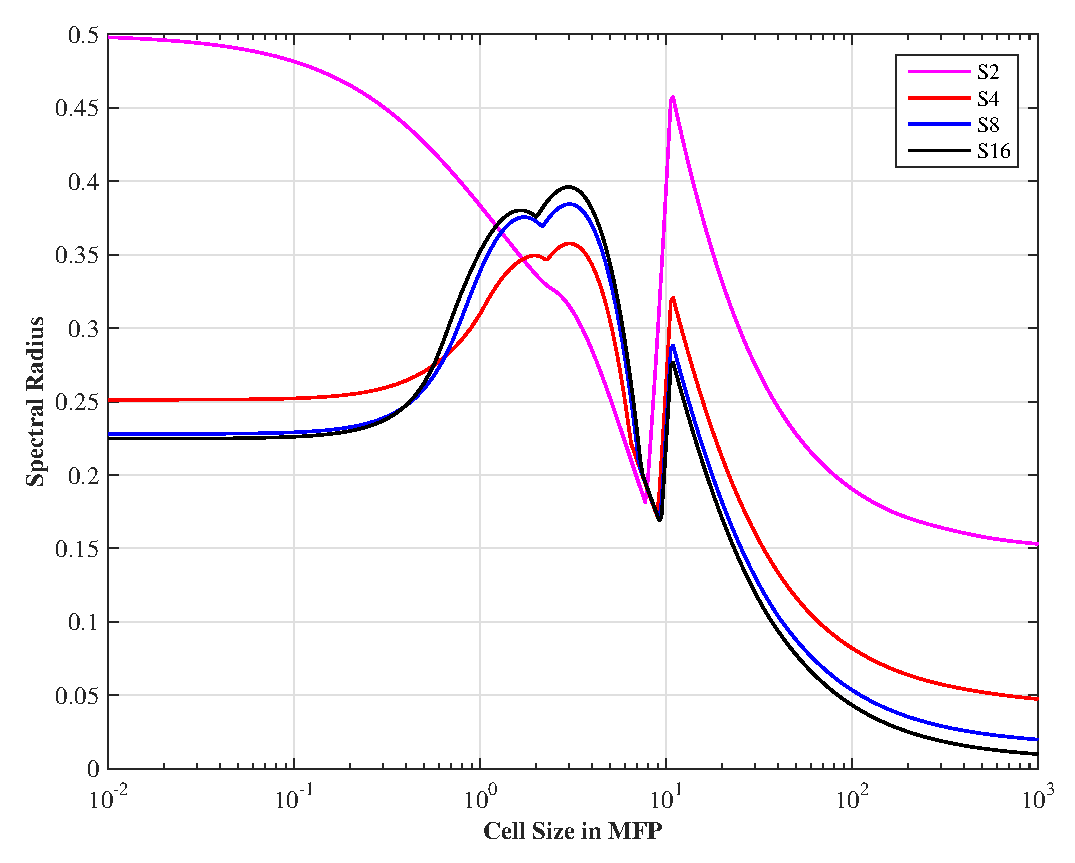
\includegraphics[width=0.95\textwidth]{figures/sec_DSA/SI_MIP_quad_C=4_UWACHSPRESS1_LS.eps}
		%\caption{Linear}
	\end{subfigure}
	\vfill
	\begin{subfigure}[b]{0.80\textwidth}
		\centering
		\includegraphics[width=0.95\textwidth]{figures/sec_DSA/SI_MIP_quad_C=4_UWACHSPRESS2_LS.eps}
		%\caption{}
	\end{subfigure}
\caption{Fourier analysis of the 2D MIP form with $c=4$ and using the linear (top) and quadratic (bottom) Wachspress basis functions.}
\label{fig::DSA_2D1G_Fourier_Wach}
\end{figure}

\begin{figure}
\centering
	\begin{subfigure}[b]{0.80\textwidth}
		\centering
		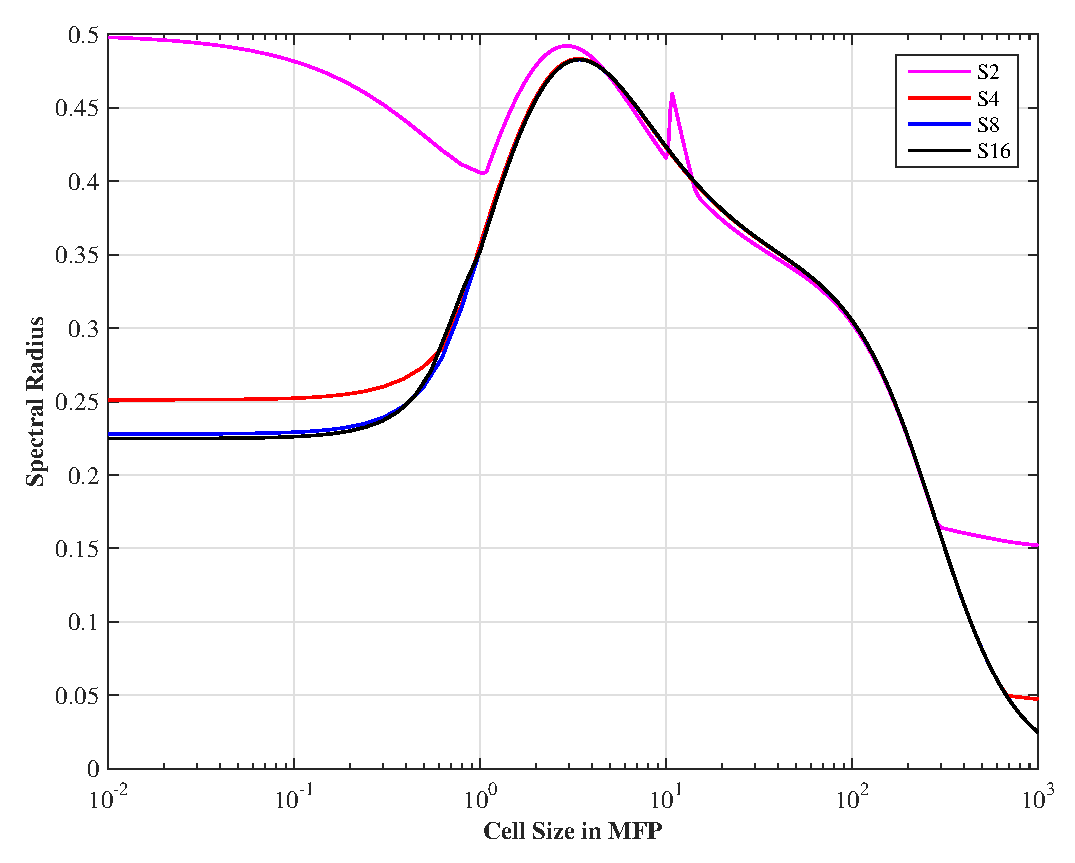
\includegraphics[width=0.95\textwidth]{figures/sec_DSA/SI_MIP_quad_C=4_PWLD1_LS.eps}
		%\caption{Linear}
	\end{subfigure}
	\vfill
	\begin{subfigure}[b]{0.80\textwidth}
		\centering
		\includegraphics[width=0.95\textwidth]{figures/sec_DSA/SI_MIP_quad_C=4_UPWLD2_LS.eps}
		%\caption{}
	\end{subfigure}
\caption{Fourier analysis of the 2D MIP form with $c=4$ and using the linear (top) and quadratic (bottom) PWL basis functions.}
\label{fig::DSA_2D1G_Fourier_PWL}
\end{figure}

\begin{figure}
\centering
	\begin{subfigure}[b]{0.80\textwidth}
		\centering
		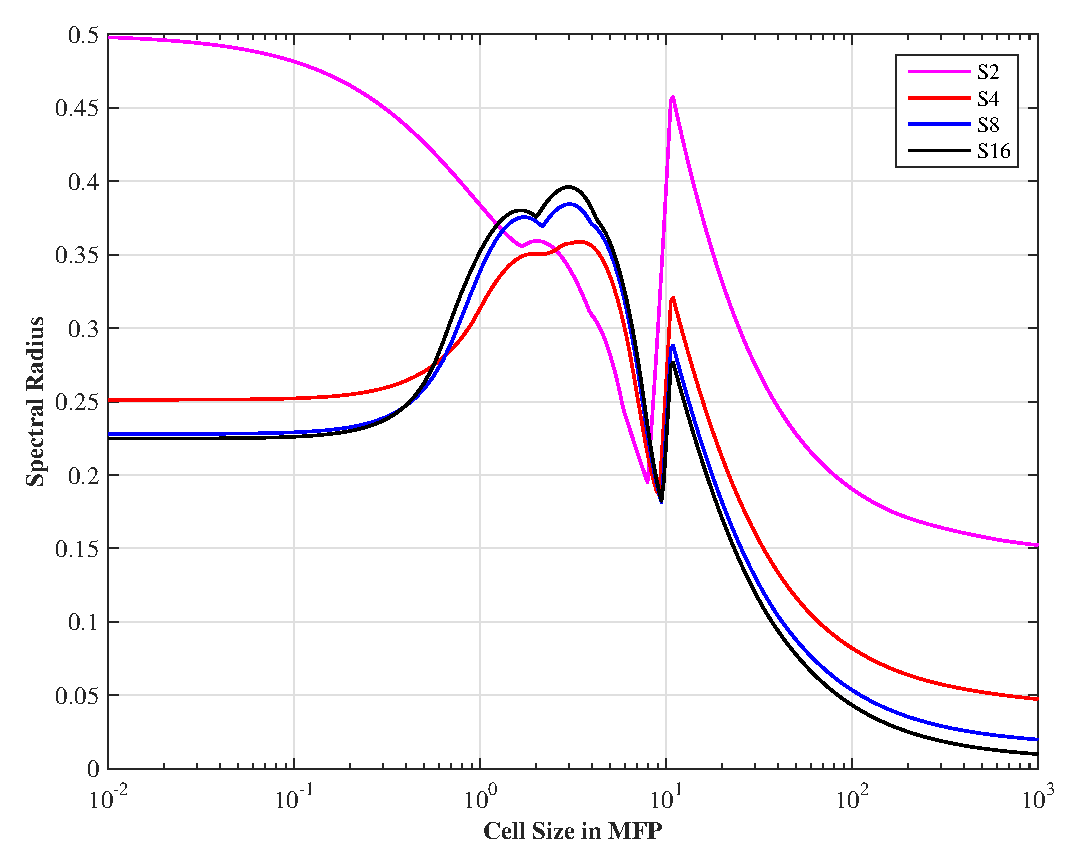
\includegraphics[width=0.95\textwidth]{figures/sec_DSA/SI_MIP_quad_C=4_UMV1_LS.eps}
		%\caption{Linear}
	\end{subfigure}
	\vfill
	\begin{subfigure}[b]{0.80\textwidth}
		\centering
		\includegraphics[width=0.95\textwidth]{figures/sec_DSA/SI_MIP_quad_C=4_UMV2_LS.eps}
		%\caption{}
	\end{subfigure}
\caption{Fourier analysis of the 2D MIP form with $c=4$ and using the linear (top) and quadratic (bottom) mean value basis functions.}
\label{fig::DSA_2D1G_Fourier_MV}
\end{figure}

\begin{figure}
\centering
	\begin{subfigure}[b]{0.80\textwidth}
		\centering
		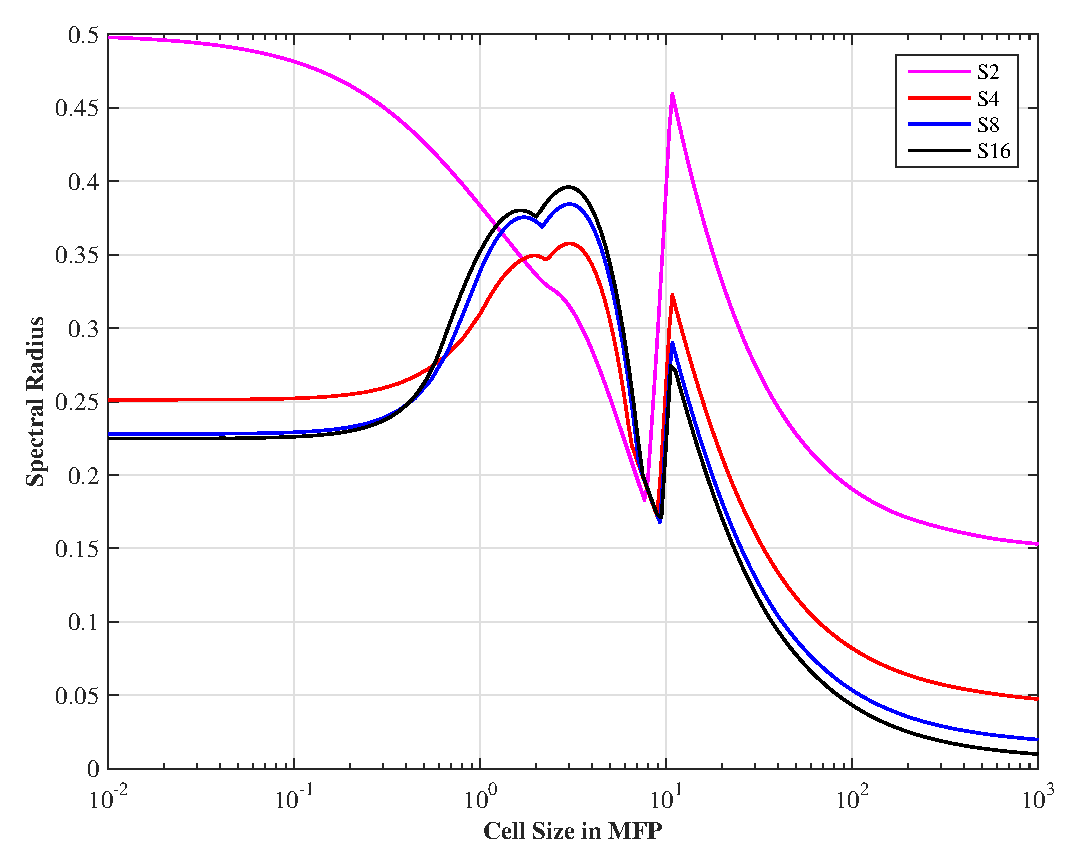
\includegraphics[width=0.95\textwidth]{figures/sec_DSA/SI_MIP_quad_C=4_MAXENT1_LS.eps}
		%\caption{Linear}
	\end{subfigure}
	\vfill
	\begin{subfigure}[b]{0.80\textwidth}
		\centering
		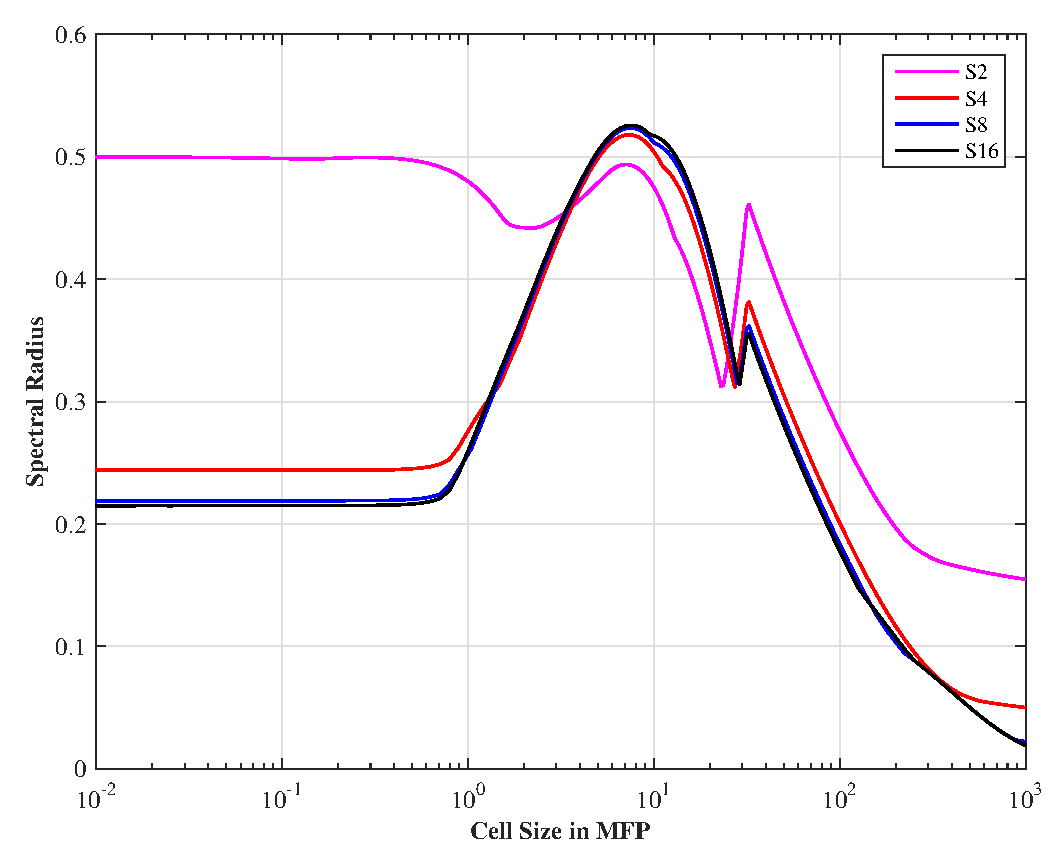
\includegraphics[width=0.95\textwidth]{figures/sec_DSA/SI_MIP_quad_C=4_UMAXENT2_LS.eps}
		%\caption{}
	\end{subfigure}
\caption{Fourier analysis of the 2D MIP form with $c=4$ and using the linear (top) and quadratic (bottom) maximum entropy basis functions.}
\label{fig::DSA_2D1G_Fourier_ME}
\end{figure}

\begin{figure}
\centering
	{
	\begin{subfigure}[b]{0.485\textwidth}
		\centering
		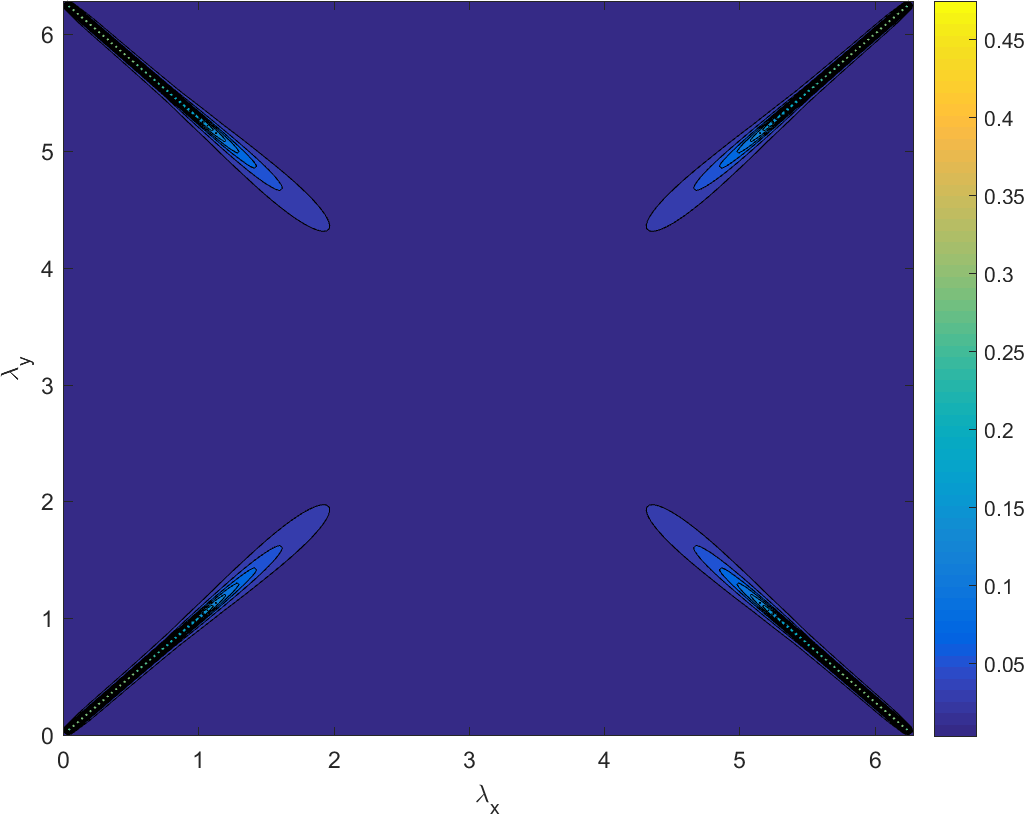
\includegraphics[width=0.975\textwidth]{figures/sec_DSA/SI_MIP_C=4_UPWLD1_LS2_x=1e-2_dydx=1_contour.png}
		\caption{$10^{-2}$ mfp}
	\end{subfigure}
	\hfill
	\begin{subfigure}[b]{0.485\textwidth}
		\centering
		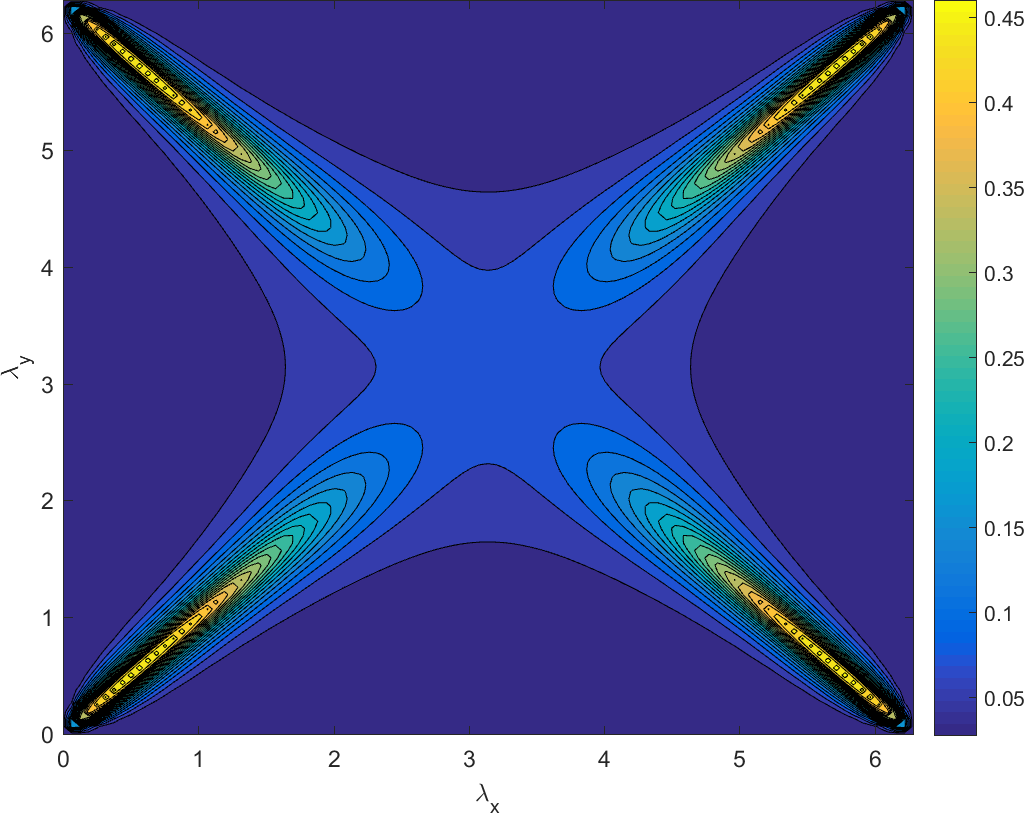
\includegraphics[width=0.975\textwidth]{figures/sec_DSA/SI_MIP_C=4_UPWLD1_LS2_x=1e-1_dydx=1_contour.png}
		\caption{$10^{-1}$ mfp}
	\end{subfigure}
	}
	\vspace{0.5cm}
	{
	\begin{subfigure}[b]{0.485\textwidth}
		\centering
		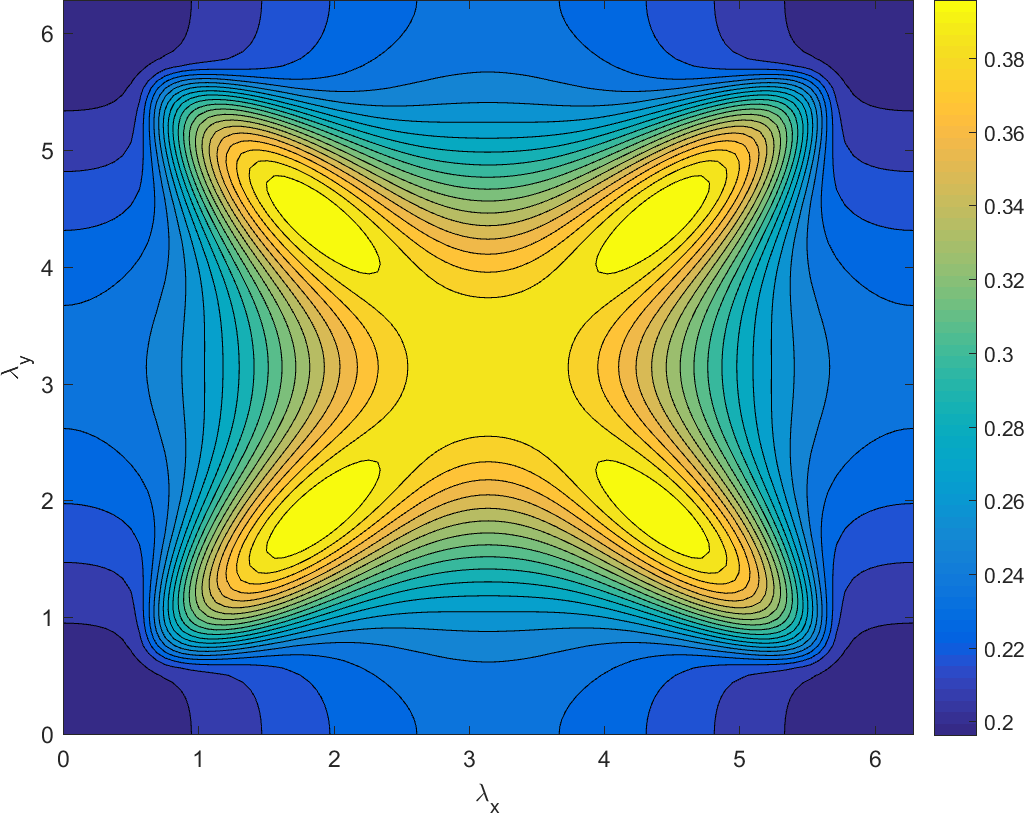
\includegraphics[width=0.975\textwidth]{figures/sec_DSA/SI_MIP_C=4_UPWLD1_LS2_x=1_dydx=1_contour.png}
		\caption{$10^{0}$ mfp}
	\end{subfigure}
	\hfill
	\begin{subfigure}[b]{0.485\textwidth}
		\centering
		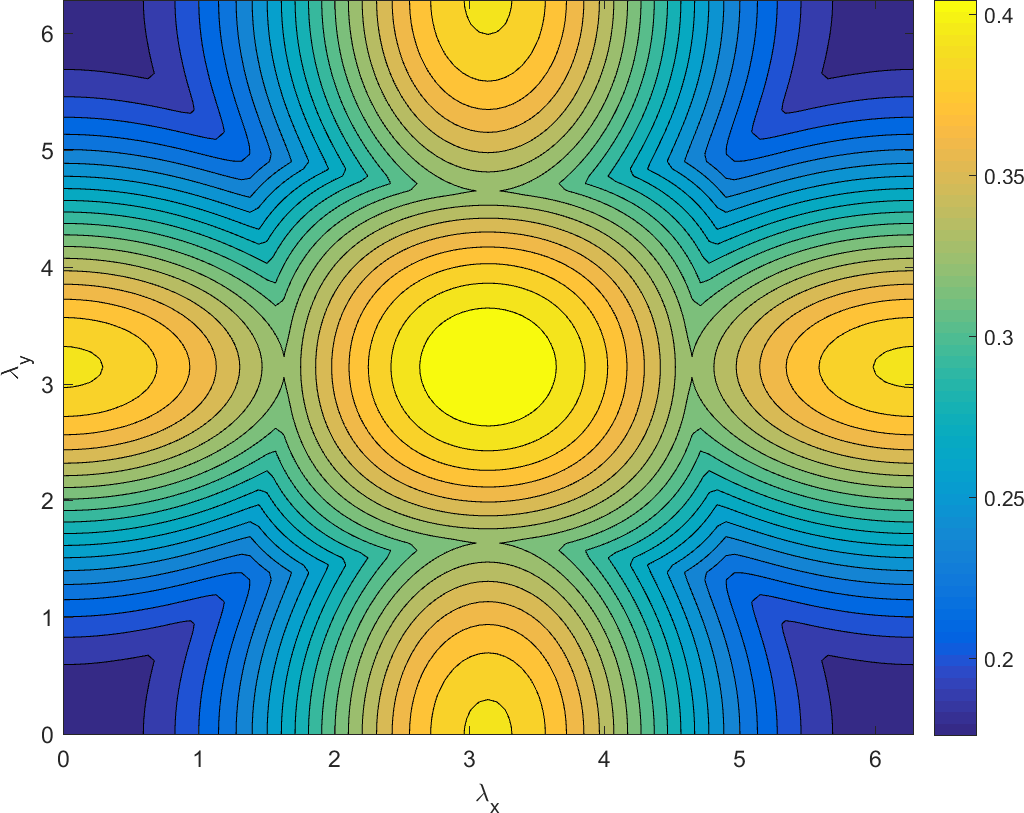
\includegraphics[width=0.975\textwidth]{figures/sec_DSA/SI_MIP_C=4_UPWLD1_LS2_x=10_dydx=1_contour.png}
		\caption{$10^{1}$ mfp}
	\end{subfigure}
	}
	\vspace{0.5cm}
	{
	\begin{subfigure}[b]{0.485\textwidth}
		\centering
		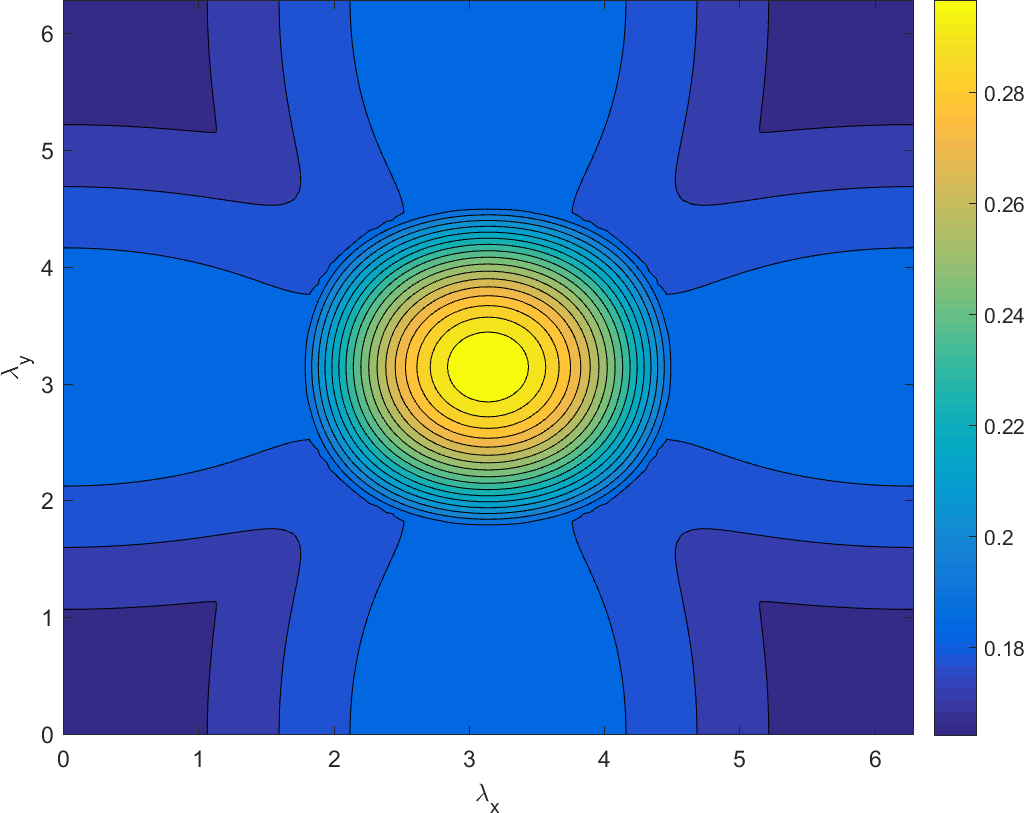
\includegraphics[width=0.975\textwidth]{figures/sec_DSA/SI_MIP_C=4_UPWLD1_LS2_x=100_dydx=1_contour.png}
		\caption{$10^{2}$ mfp}
	\end{subfigure}
	\hfill
	\begin{subfigure}[b]{0.485\textwidth}
		\centering
		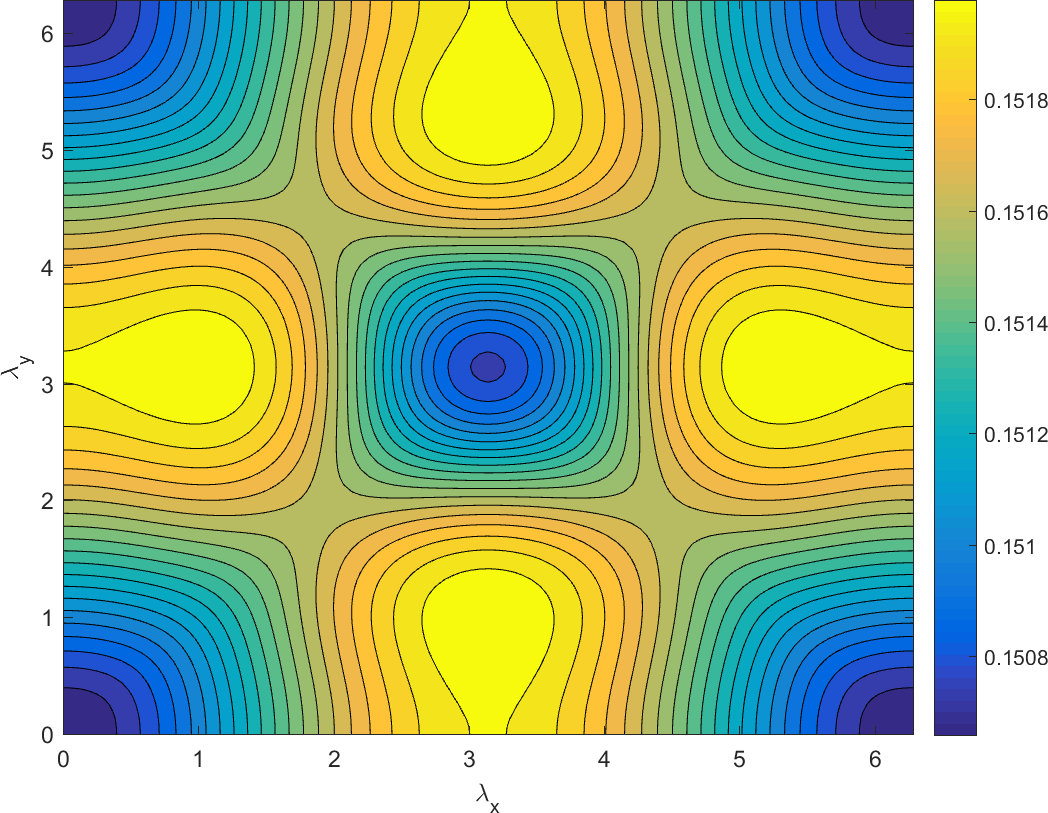
\includegraphics[width=0.975\textwidth]{figures/sec_DSA/SI_MIP_C=4_UPWLD1_LS2_x=1000_dydx=1_contour.png}
		\caption{$10^{3}$ mfp}
	\end{subfigure}
	}
\caption{Fourier wave number distribution for different mesh optical thicknesses of a single 2D square cell with PWL basis functions and $LS_{2}$ quadrature.}
\label{fig::2D_homo_dsa_wave_LS2}
\end{figure}

\begin{figure}
\centering
	{
	\begin{subfigure}[b]{0.485\textwidth}
		\centering
		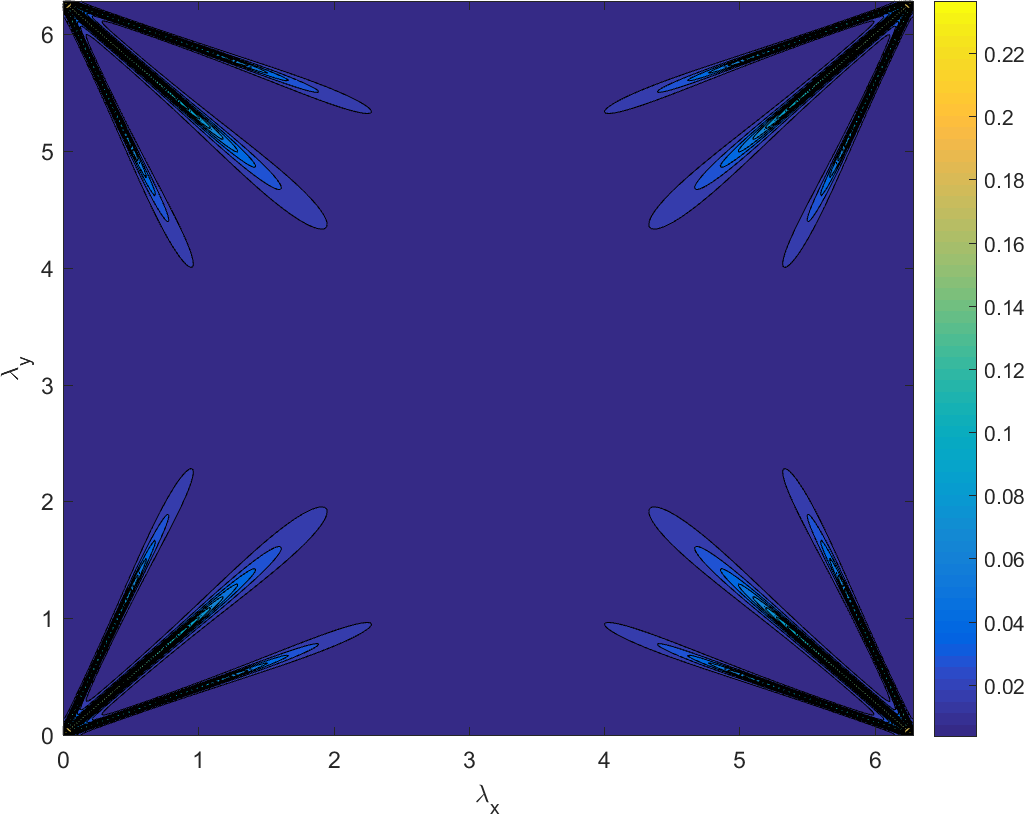
\includegraphics[width=0.975\textwidth]{figures/sec_DSA/SI_MIP_C=4_UPWLD1_LS4_x=1e-2_dydx=1_contour.png}
		\caption{$10^{-2}$ mfp}
	\end{subfigure}
	\hfill
	\begin{subfigure}[b]{0.485\textwidth}
		\centering
		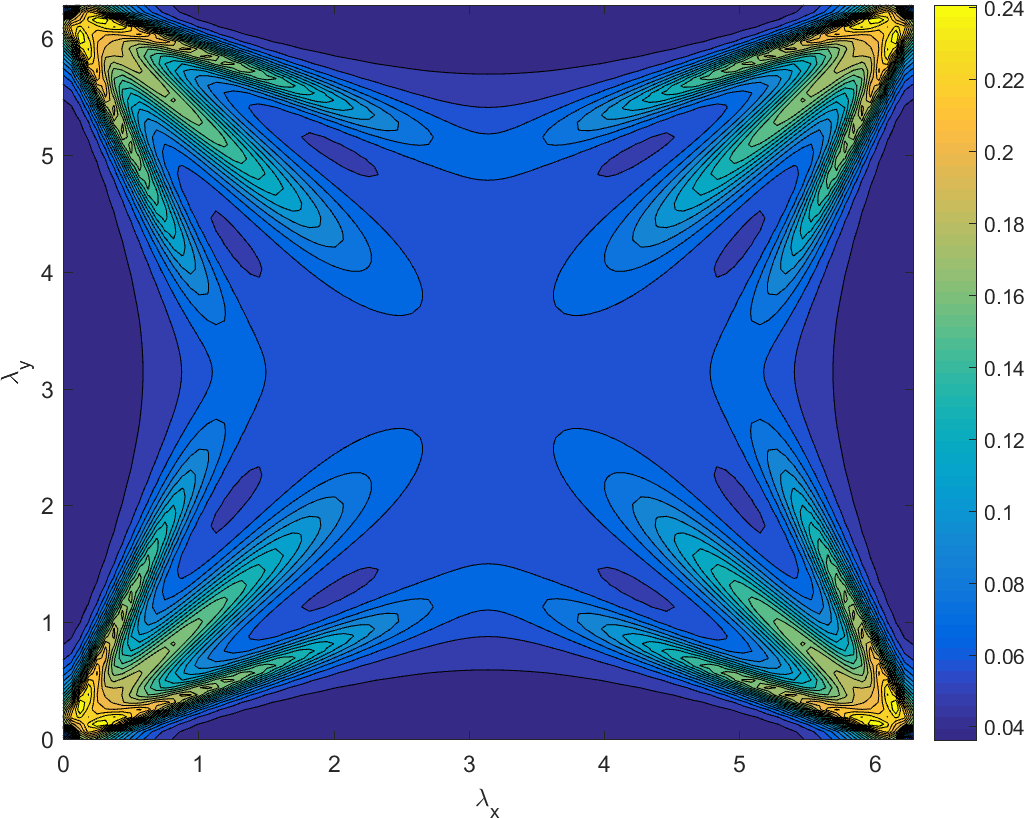
\includegraphics[width=0.975\textwidth]{figures/sec_DSA/SI_MIP_C=4_UPWLD1_LS4_x=1e-1_dydx=1_contour.png}
		\caption{$10^{-1}$ mfp}
	\end{subfigure}
	}
	\vspace{0.5cm}
	{
	\begin{subfigure}[b]{0.485\textwidth}
		\centering
		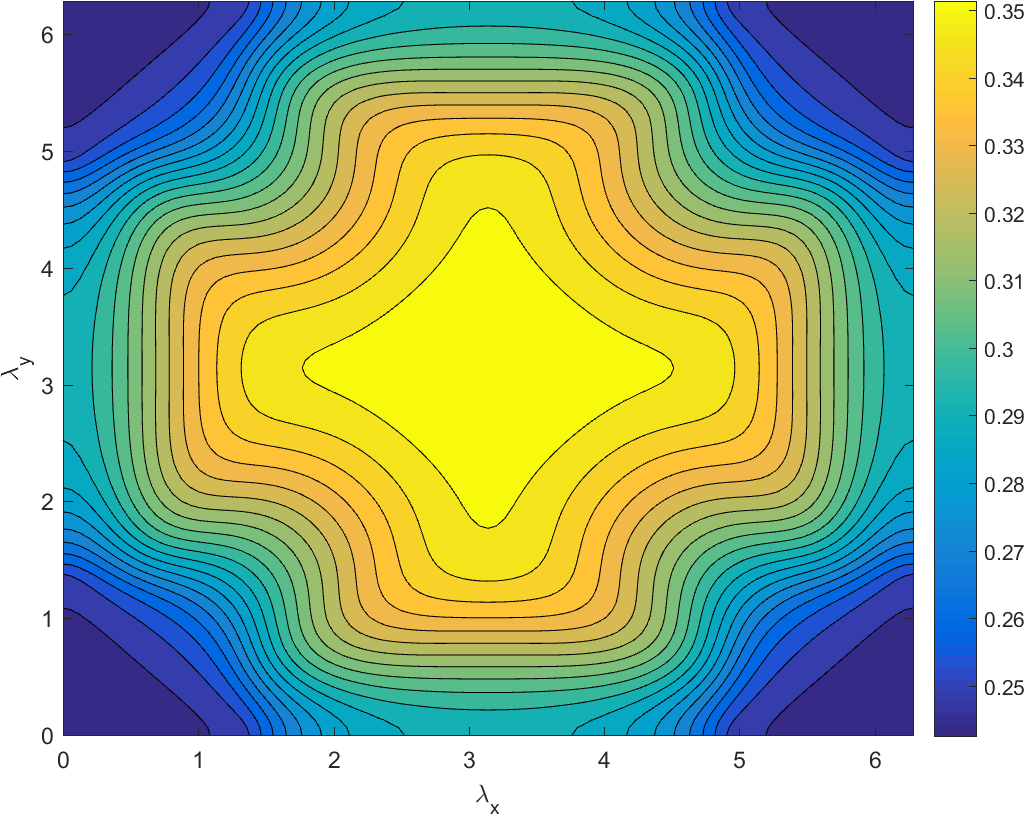
\includegraphics[width=0.975\textwidth]{figures/sec_DSA/SI_MIP_C=4_UPWLD1_LS4_x=1_dydx=1_contour.png}
		\caption{$10^{0}$ mfp}
	\end{subfigure}
	\hfill
	\begin{subfigure}[b]{0.485\textwidth}
		\centering
		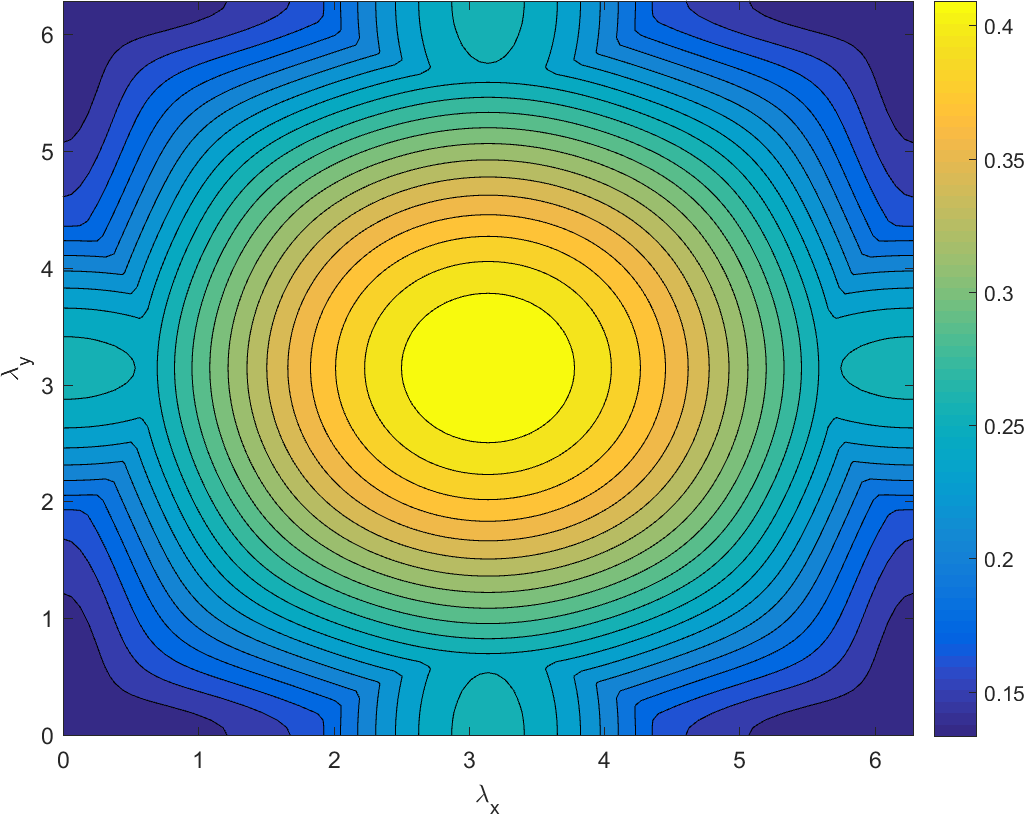
\includegraphics[width=0.975\textwidth]{figures/sec_DSA/SI_MIP_C=4_UPWLD1_LS4_x=10_dydx=1_contour.png}
		\caption{$10^{1}$ mfp}
	\end{subfigure}
	}
	\vspace{0.5cm}
	{
	\begin{subfigure}[b]{0.485\textwidth}
		\centering
		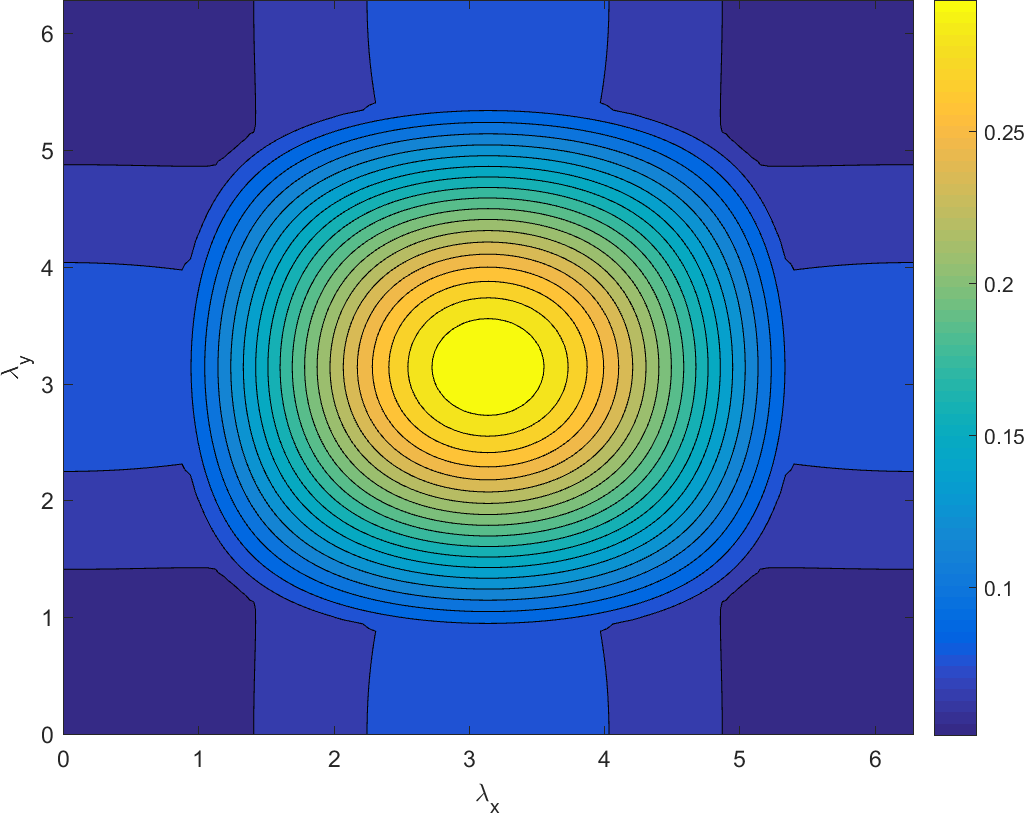
\includegraphics[width=0.975\textwidth]{figures/sec_DSA/SI_MIP_C=4_UPWLD1_LS4_x=100_dydx=1_contour.png}
		\caption{$10^{2}$ mfp}
	\end{subfigure}
	\hfill
	\begin{subfigure}[b]{0.485\textwidth}
		\centering
		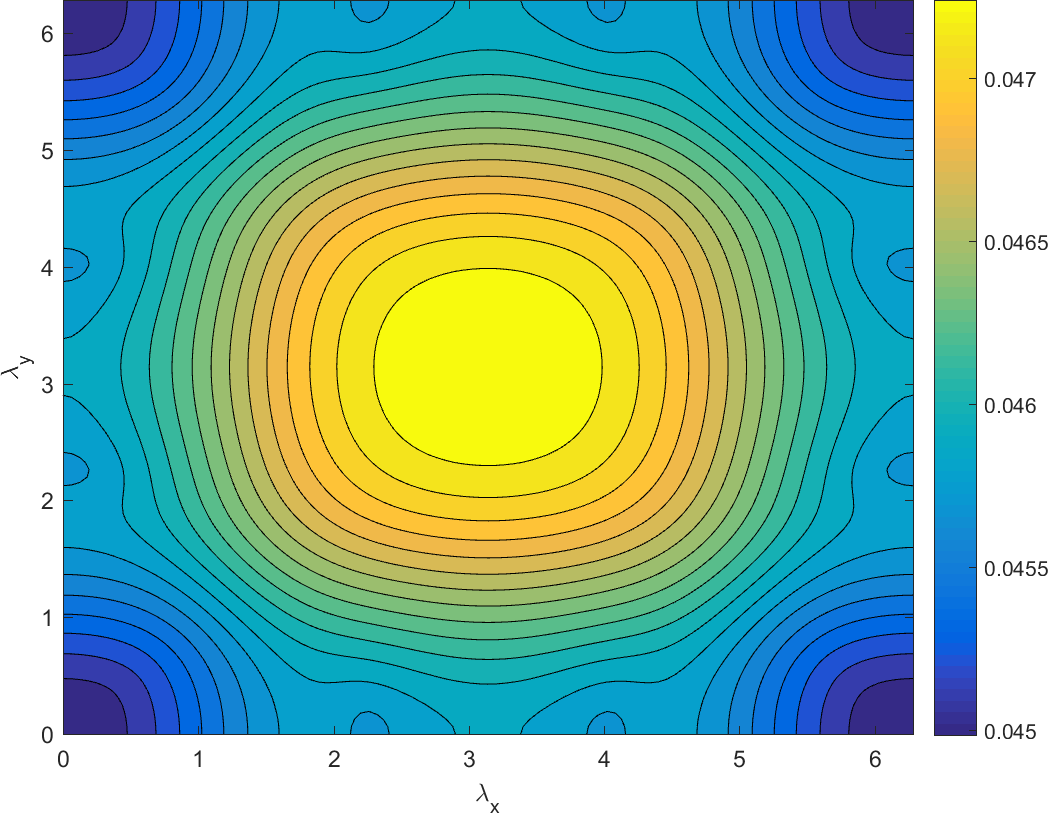
\includegraphics[width=0.975\textwidth]{figures/sec_DSA/SI_MIP_C=4_UPWLD1_LS4_x=1000_dydx=1_contour.png}
		\caption{$10^{3}$ mfp}
	\end{subfigure}
	}
\caption{Fourier wave number distribution for different mesh optical thicknesses of a single 2D square cell with PWL basis functions and $LS_{4}$ quadrature.}
\label{fig::2D_homo_dsa_wave_LS4}
\end{figure}

\begin{figure}
\centering
	{
	\begin{subfigure}[b]{0.485\textwidth}
		\centering
		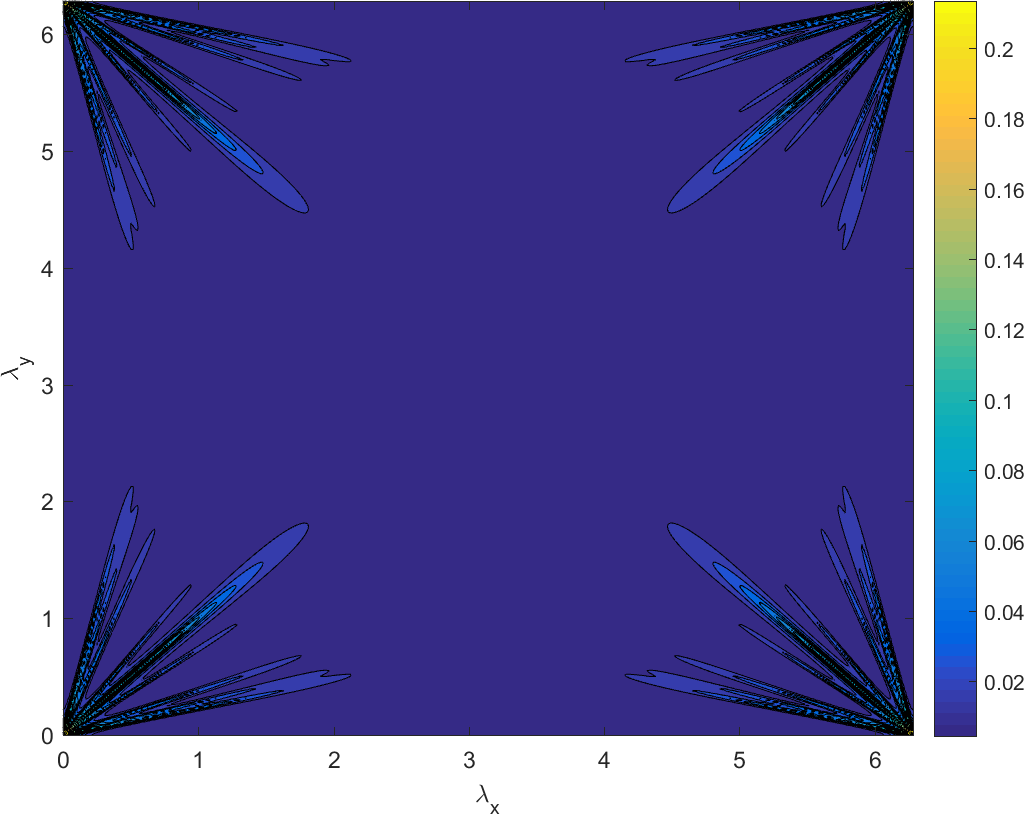
\includegraphics[width=0.975\textwidth]{figures/sec_DSA/SI_MIP_C=4_UPWLD1_LS8_x=1e-2_dydx=1_contour.png}
		\caption{$10^{-2}$ mfp}
	\end{subfigure}
	\hfill
	\begin{subfigure}[b]{0.485\textwidth}
		\centering
		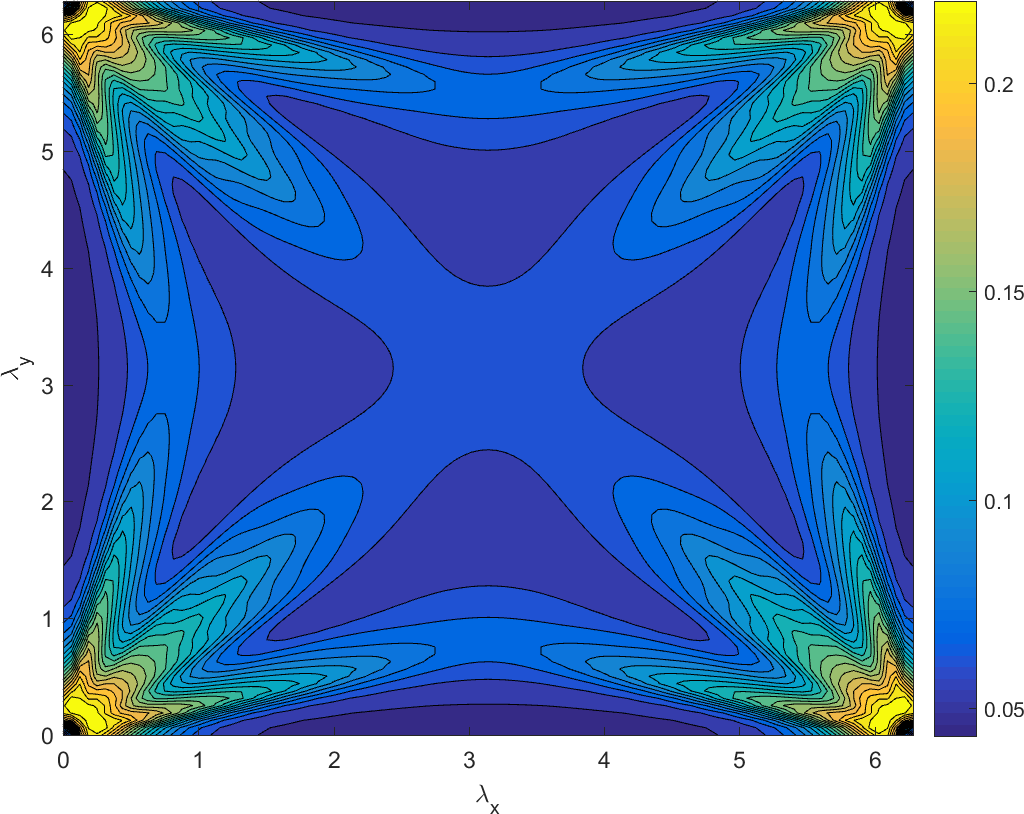
\includegraphics[width=0.975\textwidth]{figures/sec_DSA/SI_MIP_C=4_UPWLD1_LS8_x=1e-1_dydx=1_contour.png}
		\caption{$10^{-1}$ mfp}
	\end{subfigure}
	}
	\vspace{0.5cm}
	{
	\begin{subfigure}[b]{0.485\textwidth}
		\centering
		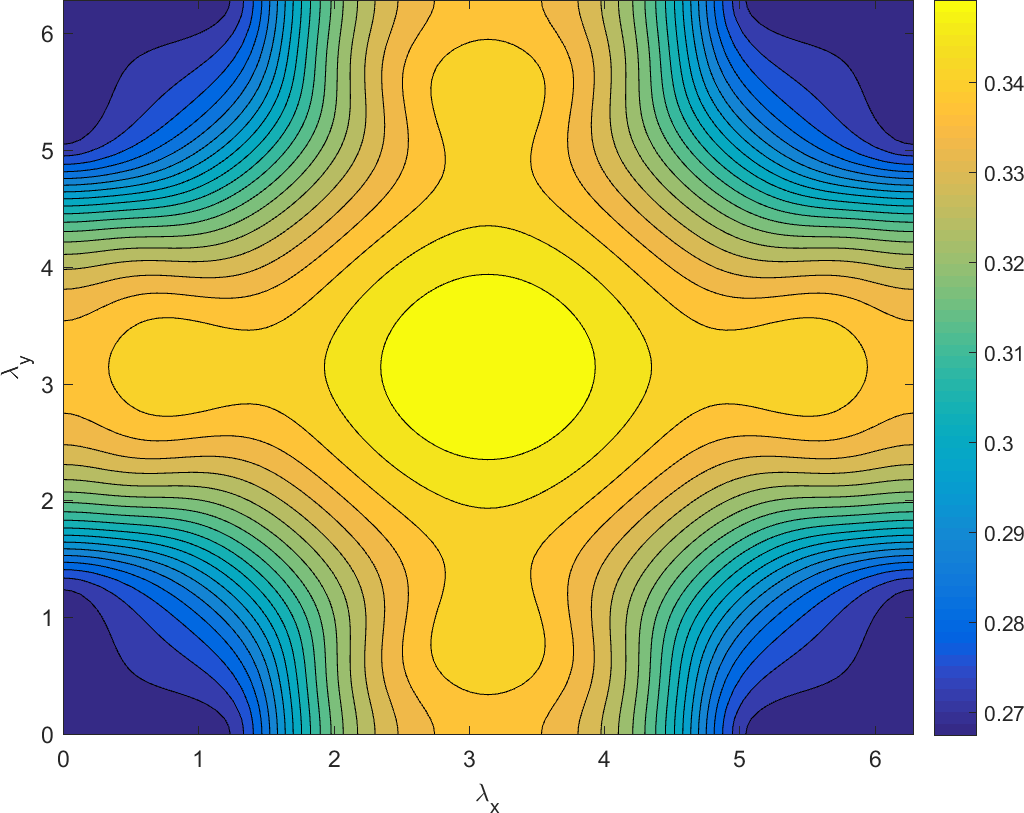
\includegraphics[width=0.975\textwidth]{figures/sec_DSA/SI_MIP_C=4_UPWLD1_LS8_x=1_dydx=1_contour.png}
		\caption{$10^{0}$ mfp}
	\end{subfigure}
	\hfill
	\begin{subfigure}[b]{0.485\textwidth}
		\centering
		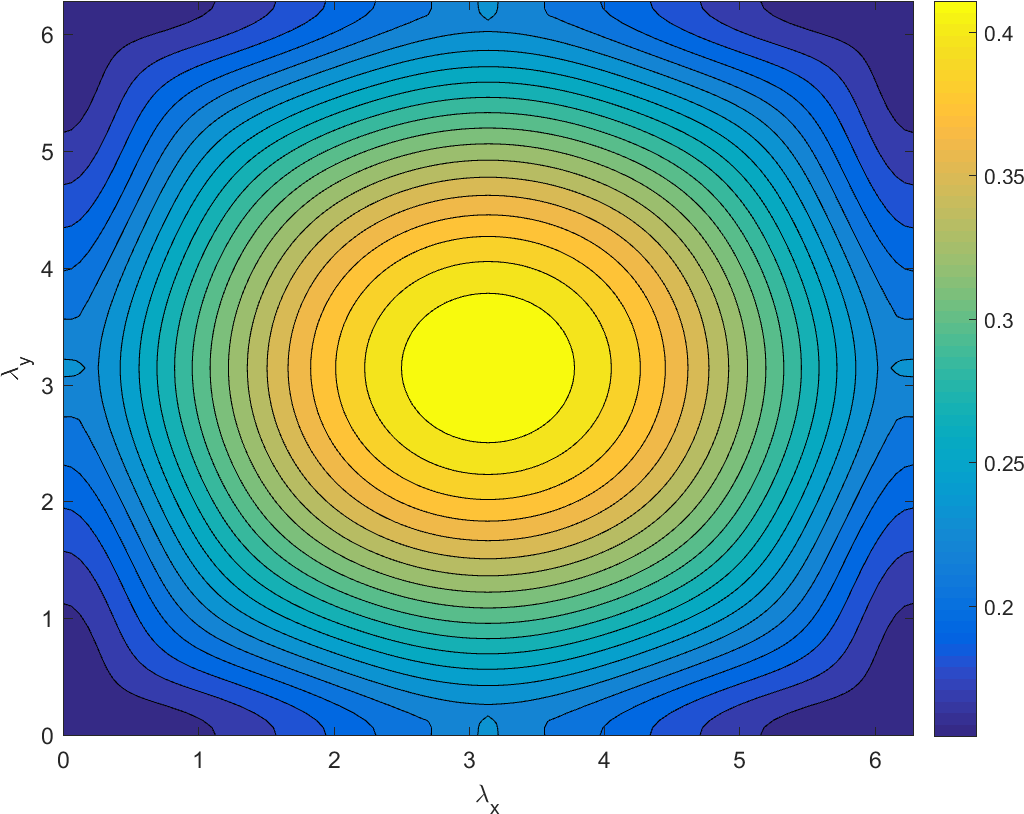
\includegraphics[width=0.975\textwidth]{figures/sec_DSA/SI_MIP_C=4_UPWLD1_LS8_x=10_dydx=1_contour.png}
		\caption{$10^{1}$ mfp}
	\end{subfigure}
	}
	\vspace{0.5cm}
	{
	\begin{subfigure}[b]{0.485\textwidth}
		\centering
		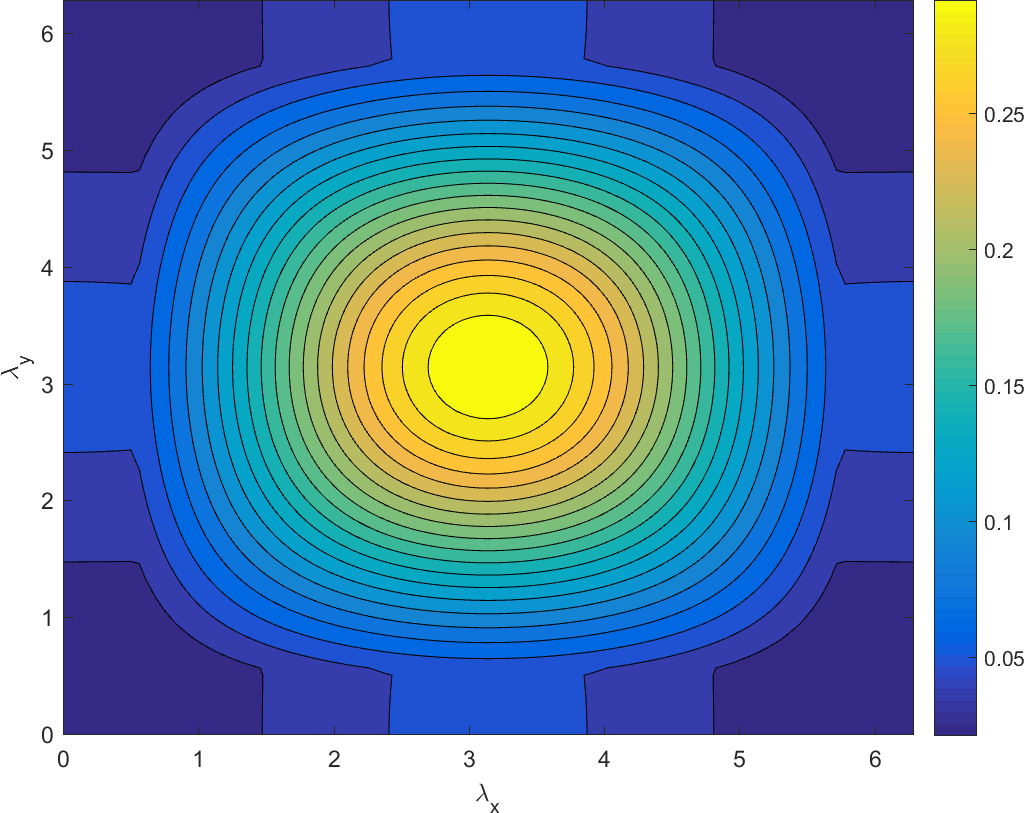
\includegraphics[width=0.975\textwidth]{figures/sec_DSA/SI_MIP_C=4_UPWLD1_LS8_x=100_dydx=1_contour.png}
		\caption{$10^{2}$ mfp}
	\end{subfigure}
	\hfill
	\begin{subfigure}[b]{0.485\textwidth}
		\centering
		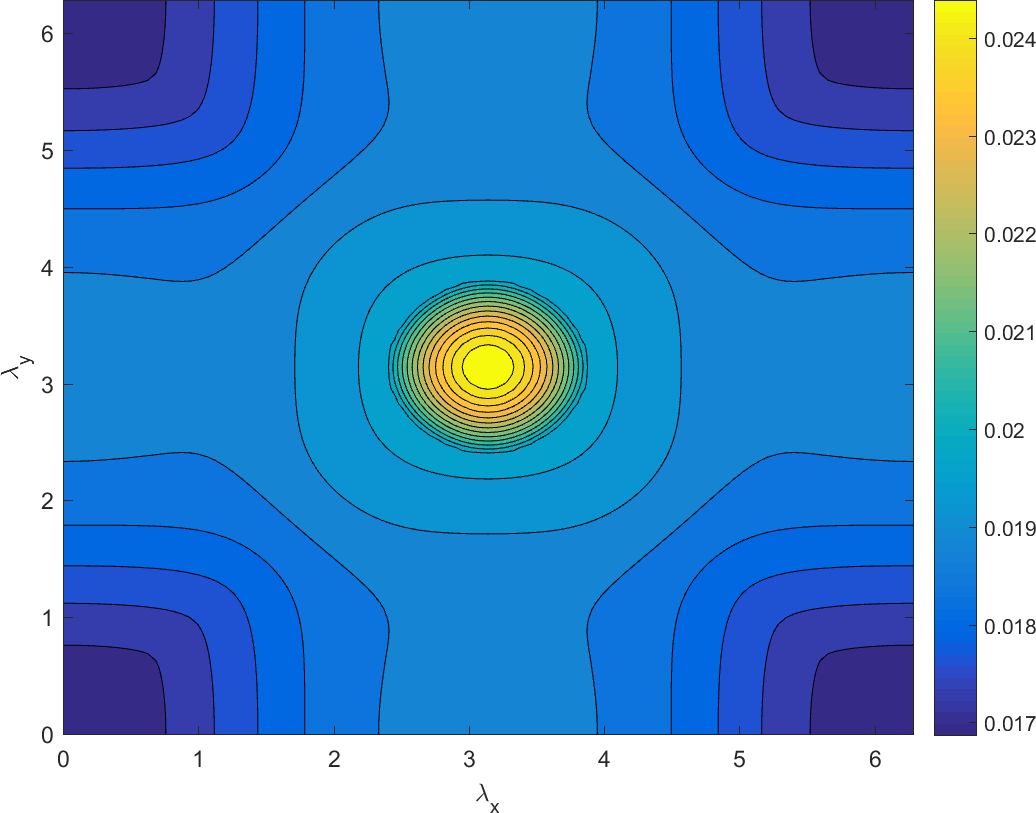
\includegraphics[width=0.975\textwidth]{figures/sec_DSA/SI_MIP_C=4_UPWLD1_LS8_x=1000_dydx=1_contour.png}
		\caption{$10^{3}$ mfp}
	\end{subfigure}
	}
\caption{Fourier wave number distribution for different mesh optical thicknesses of a single 2D square cell with PWL basis functions and $LS_{8}$ quadrature.}
\label{fig::2D_homo_dsa_wave_LS8}
\end{figure}

\begin{figure}
\centering
	{
	\begin{subfigure}[b]{0.485\textwidth}
		\centering
		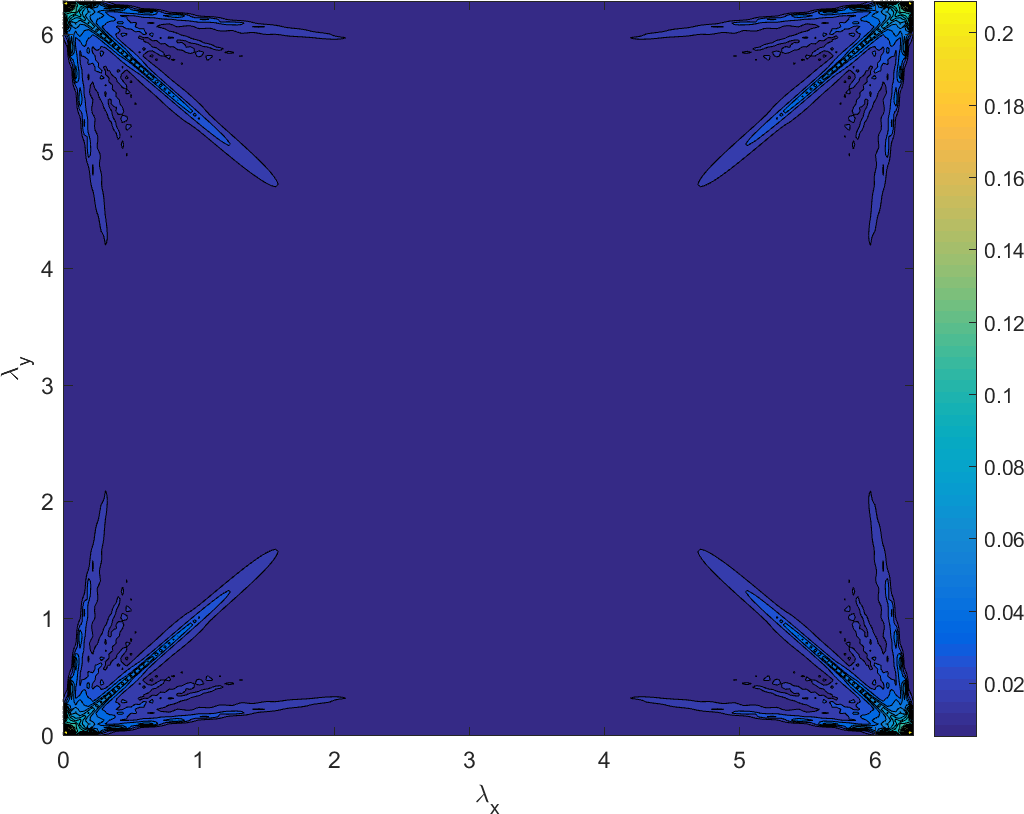
\includegraphics[width=0.975\textwidth]{figures/sec_DSA/SI_MIP_C=4_UPWLD1_LS16_x=1e-2_dydx=1_contour.png}
		\caption{$10^{-2}$ mfp}
	\end{subfigure}
	\hfill
	\begin{subfigure}[b]{0.485\textwidth}
		\centering
		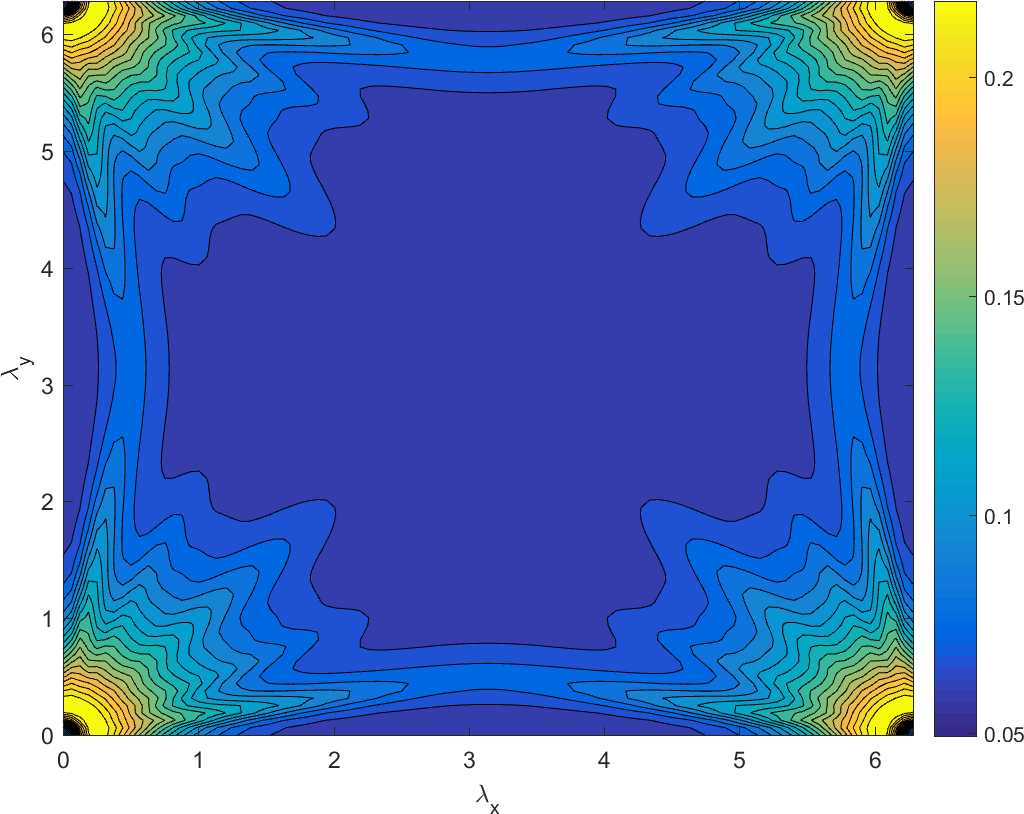
\includegraphics[width=0.975\textwidth]{figures/sec_DSA/SI_MIP_C=4_UPWLD1_LS16_x=1e-1_dydx=1_contour.png}
		\caption{$10^{-1}$ mfp}
	\end{subfigure}
	}
	\vspace{0.5cm}
	{
	\begin{subfigure}[b]{0.485\textwidth}
		\centering
		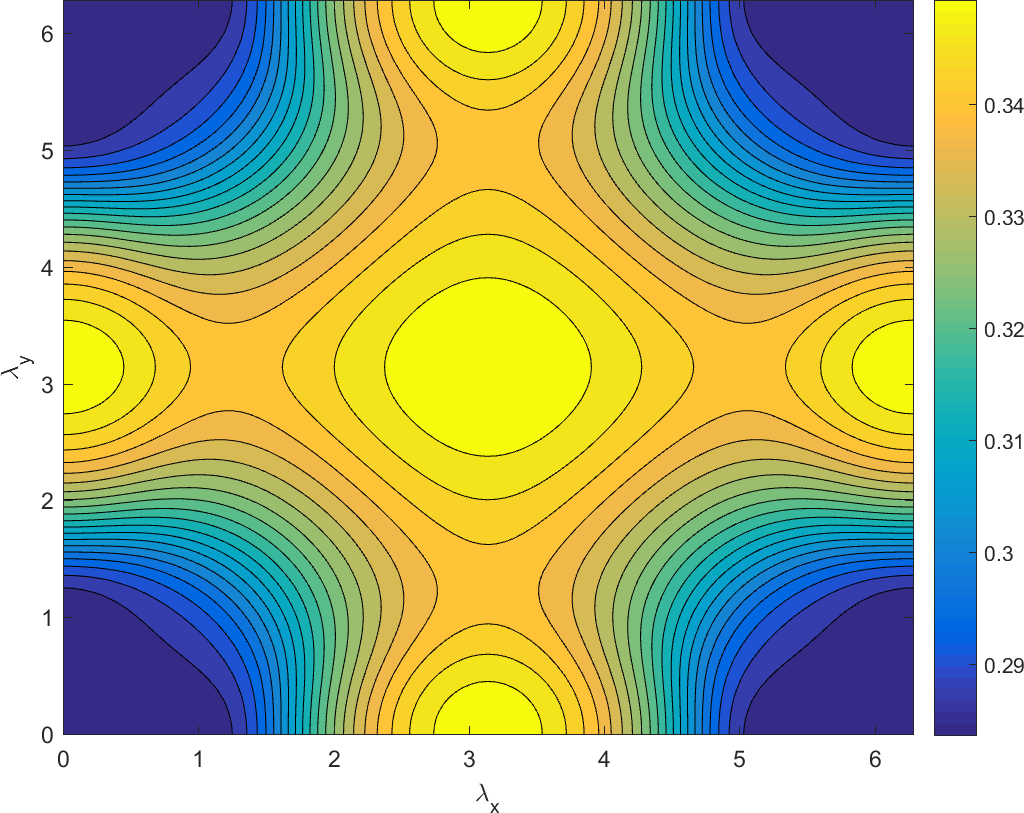
\includegraphics[width=0.975\textwidth]{figures/sec_DSA/SI_MIP_C=4_UPWLD1_LS16_x=1_dydx=1_contour.png}
		\caption{$10^{0}$ mfp}
	\end{subfigure}
	\hfill
	\begin{subfigure}[b]{0.485\textwidth}
		\centering
		\includegraphics[width=0.975\textwidth]{figures/sec_DSA/SI_MIP_C=4_UPWLD1_LS16_x=10_dydx=1_contour.png}
		\caption{$10^{1}$ mfp}
	\end{subfigure}
	}
	\vspace{0.5cm}
	{
	\begin{subfigure}[b]{0.485\textwidth}
		\centering
		\includegraphics[width=0.975\textwidth]{figures/sec_DSA/SI_MIP_C=4_UPWLD1_LS16_x=100_dydx=1_contour.png}
		\caption{$10^{2}$ mfp}
	\end{subfigure}
	\hfill
	\begin{subfigure}[b]{0.485\textwidth}
		\centering
		\includegraphics[width=0.975\textwidth]{figures/sec_DSA/SI_MIP_C=4_UPWLD1_LS16_x=1000_dydx=1_contour.png}
		\caption{$10^{3}$ mfp}
	\end{subfigure}
	}
\caption{Fourier wave number distribution for different mesh optical thicknesses of a single 2D square cell with PWL basis functions and $LS_{16}$ quadrature.}
\label{fig::2D_homo_dsa_wave_LS16}
\end{figure}


%%%%%%%%%%%%%%%%%%%%%%%%%%%%%%%%%%%%%%%%%%%%%%%%%%%
%%%   SubSubSection -  3D Homogeneous Medium
\subsubsection{3D Homogeneous Medium Case}
\label{sec::DSA_Results_1G_3DHomo}


In this Section, we perform similar analysis to that presented in Section \ref{sec::DSA_Results_1G_2DHomo}. We perform both Fourier and numerical analysis on the 3D MIP DSA scheme on homogeneous domains. The 3D PWL basis functions are used for all of the analysis presented here. First, we show results of Fourier Analysis performed on the unit cube ($X=Y=Z=1$) in Figure \ref{fig::DSA_3D1G_Fourier}. A single mesh cell is used, and the spectral radius of the FA is plotted against the cell size in terms of mean free paths. Since we only use the unit cube in this analysis, the cell sizes change by varying the total cross section. In Figure \ref{fig::DSA_3D1G_Fourier}, scattering is isotropic with a scattering ratio ($\sigma_s/\sigma_t$) of 0.9999. Level-symmetric quadrature of orders 2, 4, 8, and 16 was used and values of 1 and 4 were used for the constant in the MIP penalty coefficient, $c$. We can see from both the plots that the 3D MIP form is unconditionally stable between the two penalty coefficient constants. All spectral radii values are below 0.6 except for the case of $S_2$ quadrature with the penalty coefficient constant value of 1. This means that $c=1$ offers insufficient penalization and a higher value should be used.

\begin{figure}
\centering
	\begin{subfigure}[b]{0.80\textwidth}
		\centering
		\includegraphics[width=0.95\textwidth]{figures/sec_DSA/SI_MIP_hex_C=1_PWLD_LS.eps}
	\end{subfigure}
	\vfill
	\begin{subfigure}[b]{0.80\textwidth}
		\centering
		\includegraphics[width=0.95\textwidth]{figures/sec_DSA/SI_MIP_hex_C=4_PWLD_LS.eps}
	\end{subfigure}
\caption{Fourier spectral radius of the 3D MIP form with $c=1$ (top) and $c=4$ (bottom).}
\label{fig::DSA_3D1G_Fourier}
\end{figure}

Next, Figure \ref{fig::DSA_3D1G_Fourier_AR} provides the Fourier Analysis for cells having different aspect ratios. We change the aspect ratio by fixing $X=1$ and varying the values of $Y$ and $Z$. For these problems $Y=Z$, and we again analyze both $c=1$ and $c=4$. The aspect ratios had values of ($1/100,1/64,1/16,1,16,64,100$). Only $LS_8$ quadrature is used. We can see from the two figures that the MIP acceleration continues to be unconditionally stable on 3D hexahedral cells with high aspect ratios. 

\begin{figure}
\centering
	\begin{subfigure}[b]{0.80\textwidth}
		\centering
		\includegraphics[width=0.95\textwidth]{figures/sec_DSA/SI_MIP_hex_PWLD1_AR1.eps}
		\caption{$c=1$}
	\end{subfigure}
	\vfill
	\begin{subfigure}[b]{0.80\textwidth}
		\centering
		\includegraphics[width=0.95\textwidth]{figures/sec_DSA/SI_MIP_hex_PWLD1_AR4.eps}
		\caption{$c=4$}
	\end{subfigure}
\caption{Fourier spectral radii for MIP form with $LS_8$ quadrature on cells with different aspect ratios.}
\label{fig::DSA_3D1G_Fourier_AR}
\end{figure}

Finally, we present results that compare Fourier and numerical analyses. Figure \ref{fig::DSA_3D1G_Fourier_NSR} plots the $S_2$, $S_4$, and $S_8$ FA results from Figure \ref{fig::DSA_3D1G_Fourier} along with accompanying numerical results. The numerical problem analyzed is still the unit cube ($X=Y=Z=1$), but we now have 80 mesh cells in each dimension (as compared to Fourier Analysis which only had 1 mesh cell). We stress that a large number of mesh cells are required. Otherwise, the flux gradient at the boundary is poorly represented and additional leakage occurs. This additional leakage, which is solely due to the spatial discretization, would artifically lower the spectral radius of the numerical results. We can see from Figure \ref{fig::DSA_3D1G_Fourier_NSR} that our numerical analysis follows very closely with the results from Fourier Analysis. Discrepancies lie with quadrature sets higher than $S_2$ in the fine mesh limit, but these have been reported previously \cite{ref::DSA_wang_ragusa}.

\begin{figure}
\centering
	\begin{subfigure}[b]{0.80\textwidth}
		\centering
		\includegraphics[width=0.95\textwidth]{figures/sec_DSA/SI_MIP_hex_C=1_PWLD_LS_wNSR.eps}
	\end{subfigure}
	\vfill
	\begin{subfigure}[b]{0.80\textwidth}
		\centering
		\includegraphics[width=0.95\textwidth]{figures/sec_DSA/SI_MIP_hex_C=4_PWLD_LS_wNSR.eps}
	\end{subfigure}
\caption{Comparison between the numerical spectral radii and the theoretical Fourier Analysis spectral radii on the unit cube with $c=1$ (top) and $c=4$ (bottom).}
\label{fig::DSA_3D1G_Fourier_NSR}
\end{figure}

%%%%%%%%%%%%%%%%%%%%%%%%%%%%%%%%%%%%%%%%%%%%%%%%%%%
%%%   SubSubSection -  PHI
\subsubsection{Periodic Horizontal Interface Problem}
\label{sec::DSA_Results_1G_PHI}

When DSA is applied to multidimensional problems (2D and 3D), the preconditioning of the transport operators can degrade in the presence of heterogeneous configurations with large material discontinuities \cite{azmy2002unconditionally}. The Periodic Horizontal Interface (PHI) problem is considered a litmus test for heterogeneous DSA techniques. This problem consists of horizontal strips of alternating optically thick and optically thin materials that are 1 cell in depth. We define $\sigma_1$ as the optically thick total cross section and $\sigma_2$ as the optically thin total cross section. We then define a tuning parameter, $\sigma$, and allow the region cross sections to have the following form:

\begin{equation}
\begin{aligned}
\sigma_1 &= \sigma \\
\sigma_2 &= \frac{1}{\sigma}
\end{aligned}.
\end{equation}

\noindent We can see that increasing the value of $\sigma$ will increase the magnitude of difference between the two region cross sections. Therefore, as $\sigma$ grows large, the material discontinuities will grow which could potentially reduce the performance of our DSA scheme.

From the analysis presented in Section \ref{sec::DSA_Results_1G_2DHomo}, we showed that our different 2D linear and quadratic basis functions were robust and stable, even for mesh cells with large aspect ratios. For this PHI analysis, we concentrate on analyzing just the linear PWL coordinates as our basis functions. Just like before, we will also examine different level-symmetric quadrature sets and their effects problems with varying optical thickness. The optical thickness and diffusivity of the problem is increased by varying both $\sigma$ and the scattering ratio, $c$. This study was conducted with the sequence, $\sigma = \left[ 10, 20, 40, 80, 160, 320, 640  \right]$, and with following scattering ratios: $c = \left[ 0.9,0.99,0.999,0.9999,0.99999,0.999999  \right]$.

The full results of this PHI analysis are presented in Tables \ref{tab::DSA_2DPHI_LS2} - \ref{tab::DSA_2DPHI_LS16} for the LS2, LS4, LS8, and LS16 quadratures, respectively. From these tables, we can see that MIP DSA loses its effectiveness as the heterogeneity and overall diffusivity of the problem increases. The theoretical spectral radii are greater than any of the values presented for the homogeneous case from Figure \ref{fig::DSA_1G_Fourier_PWL1}. This result is true even for the example with the smallest heterogeneity and smallest diffusivity ($\sigma=10$ and $c=0.9$). We can gain some more knowledge of the DSA degradation by observing the eigenvalue dependency on the Fourier wave numbers for our problems. Figure \ref{fig::PHI_sig=10_c=0.9} provides the eigenvalue distribution based off the Fourier wave numbers for the different quadrature sets for $\sigma=10$ and $c=0.9$. Figure \ref{fig::PHI_sig=640_c=0.9999} then provides the same information for $\sigma=640$ and $c=0.9999$.

\begin{table}
\caption{Spectral radius for the 2D PHI problem with the PWL basis functions and LS2 quadrature.}
\begin{center}
\def\arraystretch{1.6}
\begin{tabular}{|c|c|c|c|c|c|c|}
\hline
& \multicolumn{6}{c}{Scattering ratios}\vline\\
\hline
$\sigma$ & 0.9 & 0.99& 0.999& 0.9999& 0.99999& 0.99999 \\
\hline
10  &0.77091&0.89908&0.91279&0.91417&0.91431&0.91432 \\
20  &0.82038&0.94425&0.95859&0.96003&0.96018&0.96019  \\
40  &0.84803&0.96525&0.97982&0.98129&0.98144&0.98145  \\
80  &0.86188&0.97491&0.98955&0.99102&0.99117&0.99119  \\
160&0.87134&0.98003&0.99409&0.99557&0.99571&0.99573  \\
320&0.87833&0.98353&0.99626&0.99774&0.99789&0.99790  \\
640&0.88187&0.98533&0.99732&0.99880&0.99894&0.99896  \\
\hline
\end{tabular}
\end{center}
\label{tab::DSA_2DPHI_LS2}
\end{table}

\begin{table}
\caption{Spectral radius for the 2D PHI problem with the PWL basis functions and LS4 quadrature.}
\begin{center}
\def\arraystretch{1.6}
\begin{tabular}{|c|c|c|c|c|c|c|}
\hline
& \multicolumn{6}{c}{Scattering ratios}\vline\\
\hline
$\sigma$ & 0.9 & 0.99& 0.999& 0.9999& 0.99999& 0.99999 \\
\hline
10  &0.74609&0.87284&0.88970&0.89148&0.89166&0.89167\\
20  &0.81135&0.93358&0.95001&0.95179&0.95197&0.95199\\
40  &0.84353&0.96104&0.97612&0.97781&0.97799&0.97800\\
80  &0.85865&0.97342&0.98785&0.98943&0.98960&0.98961\\
160&0.86998&0.97913&0.99335&0.99482&0.99497&0.99499\\
320&0.87767&0.98307&0.99593&0.99739&0.99753&0.99755\\
640&0.88166&0.98500&0.99717&0.99863&0.99878&0.99879\\
\hline
\end{tabular}
\end{center}
\label{tab::DSA_2DPHI_LS4}
\end{table}

\begin{table}
\caption{Spectral radius for the 2D PHI problem with the PWL basis functions and LS8 quadrature.}
\begin{center}
\def\arraystretch{1.6}
\begin{tabular}{|c|c|c|c|c|c|c|}
\hline
& \multicolumn{6}{c}{Scattering ratios}\vline\\
\hline
$\sigma$ & 0.9 & 0.99& 0.999& 0.9999& 0.99999& 0.99999 \\
\hline
10  &0.75532&0.87917&0.89780&0.89989&0.90010&0.90012\\
20  &0.81754&0.93694&0.95380&0.95581&0.95602&0.95604\\
40  &0.84681&0.96337&0.97793&0.97969&0.97988&0.97990\\
80  &0.86032&0.97459&0.98898&0.99042&0.99057&0.99058\\
160&0.86980&0.98007&0.99394&0.99540&0.99554&0.99556\\
320&0.87795&0.98354&0.99623&0.99768&0.99783&0.99784\\
640&0.88204&0.98524&0.99732&0.99878&0.99892&0.99894\\
\hline
\end{tabular}
\end{center}
\label{tab::DSA_2DPHI_LS8}
\end{table}

\begin{table}
\caption{Spectral radius for the 2D PHI problem with the PWL basis functions and LS16 quadrature.}
\begin{center}
\def\arraystretch{1.6}
\begin{tabular}{|c|c|c|c|c|c|c|}
\hline
& \multicolumn{6}{c}{Scattering ratios}\vline\\
\hline
$\sigma$ & 0.9 & 0.99& 0.999& 0.9999& 0.99999& 0.99999 \\
\hline
10  &0.75796&0.88052&0.89888&0.90097&0.90119&0.90121\\
20  &0.81903&0.93790&0.95455&0.95651&0.95671&0.95673\\
40  &0.84758&0.96387&0.97842&0.98015&0.98033&0.98035\\
80  &0.86070&0.97485&0.98924&0.99069&0.99083&0.99085\\
160&0.87025&0.98029&0.99407&0.99553&0.99567&0.99569\\
320&0.87817&0.98365&0.99629&0.99775&0.99790&0.99791\\
640&0.88216&0.98530&0.99735&0.99881&0.99896&0.99897\\
\hline
\end{tabular}
\end{center}
\label{tab::DSA_2DPHI_LS16}
\end{table}

\begin{figure}
\centering
	{
	\begin{subfigure}[b]{0.485\textwidth}
		\centering
		\includegraphics[width=0.975\textwidth]{figures/sec_DSA/PHI_SI_MIP_C=4_UPWLD1_LS2_sigt=10_c=9_contour.png}
		\caption{LS2}
	\end{subfigure}
	\hfill
	\begin{subfigure}[b]{0.485\textwidth}
		\centering
		\includegraphics[width=0.975\textwidth]{figures/sec_DSA/PHI_SI_MIP_C=4_UPWLD1_LS4_sigt=10_c=9_contour.png}
		\caption{LS4}
	\end{subfigure}
	}
	\vspace{1.5cm}
	{
	\begin{subfigure}[b]{0.485\textwidth}
		\centering
		\includegraphics[width=0.975\textwidth]{figures/sec_DSA/PHI_SI_MIP_C=4_UPWLD1_LS8_sigt=10_c=9_contour.png}
		\caption{LS8}
	\end{subfigure}
	\hfill
	\begin{subfigure}[b]{0.485\textwidth}
		\centering
		\includegraphics[width=0.975\textwidth]{figures/sec_DSA/PHI_SI_MIP_C=4_UPWLD1_LS16_sigt=10_c=9_contour.png}
		\caption{LS16}
	\end{subfigure}
	}
\caption{Fourier wave number distribution for the 2D PHI problem with $\sigma=10$ and $c=0.9$ and different level-symmetric quadratures.}
\label{fig::PHI_sig=10_c=0.9}
\end{figure}

\begin{figure}
\centering
	{
	\begin{subfigure}[b]{0.485\textwidth}
		\centering
		\includegraphics[width=0.975\textwidth]{figures/sec_DSA/PHI_SI_MIP_C=4_UPWLD1_LS2_sigt=640_c=9999_contour.png}
		\caption{LS2}
	\end{subfigure}
	\hfill
	\begin{subfigure}[b]{0.485\textwidth}
		\centering
		\includegraphics[width=0.975\textwidth]{figures/sec_DSA/PHI_SI_MIP_C=4_UPWLD1_LS4_sigt=640_c=9999_contour.png}
		\caption{LS4}
	\end{subfigure}
	}
	\vspace{1.5cm}
	{
	\begin{subfigure}[b]{0.485\textwidth}
		\centering
		\includegraphics[width=0.975\textwidth]{figures/sec_DSA/PHI_SI_MIP_C=4_UPWLD1_LS8_sigt=640_c=9999_contour.png}
		\caption{LS8}
	\end{subfigure}
	\hfill
	\begin{subfigure}[b]{0.485\textwidth}
		\centering
		\includegraphics[width=0.975\textwidth]{figures/sec_DSA/PHI_SI_MIP_C=4_UPWLD1_LS16_sigt=640_c=9999_contour.png}
		\caption{LS16}
	\end{subfigure}
	}
\caption{Fourier wave number distribution for the 2D PHI problem with $\sigma=640$ and $c=0.9999$ and different level-symmetric quadratures.}
\label{fig::PHI_sig=640_c=0.9999}
\end{figure}

%%%%%%%%%%%%%%%%%%%%%%%%%%%%%%%%%%%%%%%%%%%%%%%%%%%
%%%   SubSubSection -  AMR Iron Water
\subsubsection{Performance of MIP DSA on Polygons with Adaptive Mesh Refinement}
\label{sec::DSA_Results_1G_AMR}

For the final theoretical analysis of DSA with the MIP form, we analyze the acceleration performance when AMR is utilized on a sufficiently optically thick transport with material discontinuities. The 2D transport problem that will be examined is similar to the Iron-Water problem \cite{khalil1985nodal}. It was modified by Wang and Ragusa for use with higher-order basis functions on triangular meshes with hanging nodes \cite{ref::DSA_wang_ragusa}. We will reexamine their work on degenarate polygonal grids and not use hanging nodes. The complete geometric desciption of our problem including boundary conditions and material distributions is given in Figure \ref{fig::DSA_IW_Description}. The material properties for each region which include the total cross section, scattering ratio ($c=\sigma_s/\sigma_t$), and source strength are given in Table \ref{tab::DSA_IW_mats}. Scattering is isotropic. 

\begin{table}
\caption{Material definitions and physical properties for the Iron-Water problem.}
\centering
\def\arraystretch{1.2}
\begin{tabular}{|c|c|c|c|}
\hline
Region & $\sigma_t$ ($\text{cm}^{-1}$) & c  & S ($\text{cm}^{-3} \text{sec}^{-1}$) \\
\hline
I & 1.0 & 0.90 & 1.0 \\
\hline
II & 1.5 & 0.96 & 0.0 \\
\hline
III & 1.0 & 0.30 & 0.0\\
\hline
\end{tabular}
\label{tab::DSA_IW_mats}
\end{table}

\begin{figure}
\centering
\includegraphics[width=0.60\textwidth]{figures/sec_DSA/IW_Description.png}
\caption{Geometry description for the Iron-Water problem.}
\label{fig::DSA_IW_Description}
\end{figure}

\begin{figure}
\centering
\includegraphics[width=0.50\textwidth]{figures/sec_DSA/IW_starting_mesh.png}
\caption{Initial mesh for the Iron-Water problem.}
\label{fig::DSA_IW_starting_mesh}
\end{figure}

For this analysis, we will test multiple problem configurations. All AMR histories will be calculated form an initial starting mesh provided in Figure \ref{fig::DSA_IW_starting_mesh} where the material regions are given by the different mesh cell colors. Both linear and quadratic basis functions will be analyzed, but we only use the 2D PWL coordinates. Two different angular quadratures will be used: a $S_4$ level-symmetric (LS) quadrature and a $S_{24}^2$ PGLC quadrature. We expect additional solution discontinuities (besides those corresponding to the material discontinuities) to arise along the $S_N$ rays. Therefore, we are also performing runs using the PCLG quadrature with a high number of azimuthal angles to mitigate these $S_N$ discontinuities. We also investigate the effects of solution bootstrapping as well as the effectiveness of the five preconditioner types presented in Section \ref{sec::DSA_Solving}.

We can summarize all the different problem permutations that will be analyzed:

\begin{enumerate}
\item Linear and quadratic PWL basis functions;
\item Use of either $LS_4$ or $S_{24}^{2}$ PGLC angular quadrature;
\item Bootstrappping or reinitialization of the solution at each AMR cycle;
\item Use of five different preconditioner types: no preconditioning, Jacobi preconditioning, SSOR preconditioning, ILU preconditioning, and AGMG preconditioning.
\end{enumerate}

\noindent This means that there are four physical problem configurations (basis function order and angular quadrature). For each of these problem configurations, AMR refinement cycles either utilize solution bootstrapping or reinitialization (starting flux is all zero) and 1 of the 5 preconditioner types. Therefore, there are 40 total AMR runs required for this analysis.

We first present the tabulated data 

\begin{table}
\caption{DSA counts based on preconditioner type for the Iron-Water problem with $LS_4$ quadrature, linear basis functions, and solution reinitialization.}
\begin{center}
\def\arraystretch{1.25}
\begin{tabular}{|c|c|c|c|c|c|c|}
\hline
& & \multicolumn{5}{c}{Preconditioner Type}\vline\\
\hline
Cycle & SI Iters. & None&Jacobi&SSOR& ILU& AGMG \\
\hline
0&19&357&282&58&94&19\\
1&21&635&506&75&170&21\\
2&17&831&700&91&233&17\\
3&16&917&791&100&269&127\\
4&13&1164&1062&158&351&114\\
5&12&1787&1547&218&501&106\\
6&12&2187&1883&266&594&116\\
7&12&2407&2123&330&670&122\\
8&12&3116&2698&395&843&111\\
9&11&3176&2835&449&903&113\\
10&11&4058&3515&563&1109&112\\
11&11&4442&3821&657&1221&110\\
12&11&5378&4659&788&1495&119\\
13&11&5989&5209&860&1680&123\\
14&11&6648&5824&957&1893&123\\
15&11&7655&6640&1098&2153&130\\
16&11&7973&6934&1149&2250&134\\
17&11&9456&8200&1378&2686&139\\
18&11&10181&8890&1373&2906&145\\
19&11&11111&9716&1550&3139&143\\
20&11&11934&10494&1780&3406&143\\
21&11&12456&10940&1779&3567&135\\
22&11&13896&12308&2043&3981&144\\
23&11&15216&13531&2253&4401&146\\
24&11&15932&14188&2436&4646&144\\
\hline
\end{tabular}
\end{center}
\label{tab::DSA_IW_LS4_k1_reinit}
\end{table}

\begin{table}
\caption{DSA counts based on preconditioner type for the Iron-Water problem with $LS_4$ quadrature, linear basis functions, and solution bootstrapping.}
\begin{center}
\def\arraystretch{1.25}
\begin{tabular}{|c|c|c|c|c|c|c|}
\hline
& & \multicolumn{5}{c}{Preconditioner Type}\vline\\
\hline
Cycle & SI Iters. & None&Jacobi&SSOR& ILU& AGMG \\
\hline
0&19&357&282&58&94&19\\
1&22&675&538&73&179&22\\
2&17&787&708&78&230&17\\
3&14&788&692&74&228&118\\
4&13&1028&953&116&328&123\\
5&11&1452&1317&149&470&110\\
6&10&1592&1449&165&497&106\\
7&10&1762&1581&143&501&106\\
8&9&2335&1976&217&633&97\\
9&9&2434&1989&269&606&110\\
10&8&2775&2392&309&762&92\\
11&8&2951&2531&310&775&95\\
12&8&3570&3200&384&1029&95\\
13&8&4197&3676&363&1172&103\\
14&7&4159&3604&377&1183&92\\
15&6&3961&3529&391&1087&84\\
16&6&4301&3612&333&1198&88\\
17&7&6035&5182&498&1711&104\\
18&6&5352&4790&578&1550&93\\
19&6&5897&5156&626&1655&89\\
20&6&6343&5478&518&1758&89\\
21&6&6578&5692&661&1875&89\\
22&6&6709&6212&685&1925&92\\
23&6&8376&7213&583&2346&98\\
24&5&7051&6148&659&1937&80\\
\hline
\end{tabular}
\end{center}
\label{tab::DSA_IW_LS4_k1_boot}
\end{table}

\begin{table}
\caption{DSA counts based on preconditioner type for the Iron-Water problem with $LS_4$ quadrature, quadratic basis functions, and solution reinitialization.}
\begin{center}
\def\arraystretch{1.25}
\begin{tabular}{|c|c|c|c|c|c|c|}
\hline
& & \multicolumn{5}{c}{Preconditioner Type}\vline\\
\hline
Cycle & SI Iters. & None&Jacobi&SSOR& ILU& AGMG \\
\hline
0&18&681&553&93&108&18\\
1&14&902&750&120&202&69\\
2&14&1358&1196&163&245&78\\
3&12&1464&1277&216&265&65\\
4&12&1977&1704&283&349&60\\
5&11&2858&2379&536&494&56\\
6&11&3813&3210&714&653&66\\
7&11&4450&3784&902&779&112\\
8&11&6465&5403&1259&1105&167\\
9&11&7541&6370&1691&1328&155\\
10&11&9107&7477&1948&1557&146\\
11&11&10535&8648&2554&1793&174\\
12&11&11843&9662&2660&2016&166\\
13&11&12810&10481&2960&2167&158\\
14&11&14227&11790&3179&2451&178\\
15&11&14888&12411&3422&2598&177\\
16&11&15652&12902&3408&2690&185\\
17&11&16327&13723&4120&2820&189\\
18&11&17611&14647&4105&3006&177\\
19&11&18922&15392&4319&3192&179\\
20&11&19457&16009&4527&3304&179\\
21&11&20099&16798&5032&3467&178\\
22&11&21359&17446&5198&3599&183\\
23&11&22000&17880&5397&3702&188\\
24&11&22363&18465&5539&3815&167\\
\hline
\end{tabular}
\end{center}
\label{tab::DSA_IW_LS4_k2_reinit}
\end{table}

\begin{table}
\caption{DSA counts based on preconditioner type for the Iron-Water problem with $LS_4$ quadrature, quadratic basis functions, and solution bootstrapping.}
\begin{center}
\def\arraystretch{1.25}
\begin{tabular}{|c|c|c|c|c|c|c|}
\hline
& & \multicolumn{5}{c}{Preconditioner Type}\vline\\
\hline
Cycle & SI Iters. & None&Jacobi&SSOR& ILU& AGMG \\
\hline
0&18&681&553&93&108&18\\
1&14&885&722&84&195&70\\
2&13&1315&1132&112&246&78\\
3&11&1383&1195&170&242&66\\
4&10&1722&1451&218&292&60\\
5&10&2663&2201&326&461&61\\
6&10&3509&2971&448&611&67\\
7&9&3918&3072&386&651&102\\
8&8&4919&4070&621&837&129\\
9&8&5643&4658&776&969&117\\
10&8&6770&5639&848&1160&123\\
11&9&8430&6727&1028&1430&146\\
12&8&8611&7236&1015&1492&132\\
13&8&9382&7725&1112&1606&125\\
14&7&8915&7495&1065&1559&120\\
15&7&9646&7776&1295&1623&120\\
16&7&10235&8594&1336&1788&124\\
17&7&10577&8442&1127&1747&131\\
18&7&11190&9431&1540&1949&116\\
19&7&11867&9672&1553&2069&125\\
20&7&12494&10271&1540&2090&131\\
21&7&12724&10963&1668&2259&118\\
22&7&13367&11471&1375&2370&137\\
23&7&12816&10481&1398&2207&127\\
24&7&14850&12149&1706&2560&125\\
\hline
\end{tabular}
\end{center}
\label{tab::DSA_IW_LS4_k2_boot}
\end{table}

\begin{table}
\caption{DSA counts based on preconditioner type for the Iron-Water problem with $S_{24}^2$ PGLC quadrature, linear basis functions, and solution reinitialization.}
\begin{center}
\def\arraystretch{1.25}
\begin{tabular}{|c|c|c|c|c|c|c|}
\hline
& & \multicolumn{5}{c}{Preconditioner Type}\vline\\
\hline
Cycle & SI Iters. & None&Jacobi&SSOR& ILU& AGMG \\
\hline
0&19&360&282&55&95&19\\
1&20&592&478&70&161&20\\
2&17&794&664&90&225&122\\
3&14&958&850&123&310&117\\
4&13&1571&1386&163&443&137\\
5&12&2170&1926&259&597&124\\
6&12&2308&2075&298&668&131\\
7&11&3269&2837&416&901&131\\
8&11&3836&3376&491&1093&130\\
9&10&3853&3290&570&1072&118\\
10&10&4563&4062&694&1264&115\\
11&10&4625&4288&694&1331&119\\
12&10&4932&4458&724&1386&119\\
13&10&5028&4557&744&1422&122\\
14&10&6507&5831&968&1822&124\\
15&10&6431&5936&1021&1873&123\\
16&10&8128&6994&1212&2186&125\\
17&10&8510&7421&1276&2353&128\\
18&10&8974&8043&1198&2571&131\\
19&10&8999&8110&1226&2615&127\\
20&10&9242&8236&1447&2654&132\\
21&10&9304&8327&1367&2710&132\\
22&10&11464&10143&1807&3249&135\\
23&10&11629&10272&1815&3286&135\\
24&10&11956&10565&1974&3386&134\\
\hline
\end{tabular}
\end{center}
\label{tab::DSA_IW_PGLC24_k1_reinit}
\end{table}

\begin{table}
\caption{DSA counts based on preconditioner type for the Iron-Water problem with $S_{24}^2$ PGLC quadrature, linear basis functions, and solution bootstrapping.}
\begin{center}
\def\arraystretch{1.25}
\begin{tabular}{|c|c|c|c|c|c|c|}
\hline
& & \multicolumn{5}{c}{Preconditioner Type}\vline\\
\hline
Cycle & SI Iters. & None&Jacobi&SSOR& ILU& AGMG \\
\hline
0&19&360&282&55&95&19\\
1&21&629&512&70&171&21\\
2&16&787&681&75&227&118\\
3&13&991&875&93&298&112\\
4&11&1271&1064&121&357&128\\
5&10&1879&1682&168&508&119\\
6&10&1883&1605&177&526&115\\
7&9&2419&2168&217&675&99\\
8&8&2427&2100&271&712&88\\
9&8&2624&2325&282&720&88\\
10&7&3170&2723&327&846&82\\
11&7&3132&2700&325&874&81\\
12&7&3069&2470&332&841&79\\
13&7&3310&2850&327&933&74\\
14&7&3547&3340&418&1037&77\\
15&7&4307&3889&360&1214&76\\
16&6&4505&3992&604&1301&72\\
17&6&5036&4460&501&1425&73\\
18&6&5162&4580&544&1467&75\\
19&6&5236&4572&552&1459&69\\
20&6&5525&4849&643&1523&72\\
21&6&5597&4876&613&1579&74\\
22&6&6249&5652&770&1880&72\\
23&6&6202&5537&666&1805&72\\
24&6&5918&5375&741&1717&72\\
\hline
\end{tabular}
\end{center}
\label{tab::DSA_IW_PGLC24_k1_boot}
\end{table}

\begin{table}
\caption{DSA counts based on preconditioner type for the Iron-Water problem with $S_{24}^2$ PGLC quadrature, quadratic basis functions, and solution reinitialization.}
\begin{center}
\def\arraystretch{1.25}
\begin{tabular}{|c|c|c|c|c|c|c|}
\hline
& & \multicolumn{5}{c}{Preconditioner Type}\vline\\
\hline
Cycle & SI Iters. & None&Jacobi&SSOR& ILU& AGMG \\
\hline
0&17&432&518&47&109&19\\
1&16&710&592&76&192&79\\
2&15&953&794&144&219&84\\
3&13&1150&958&197&239&70\\
4&14&1885&1571&261&339&70\\
5&13&2604&2170&414&487&66\\
6&12&2770&2308&477&594&72\\
7&12&3923&3269&666&708&122\\
8&11&4603&3836&786&921&167\\
9&10&4624&3853&912&1006&141\\
10&10&5476&4563&1110&1180&133\\
11&10&5550&4625&1110&1358&158\\
12&10&5918&4932&1158&1527&151\\
13&10&6034&5028&1190&1642&144\\
14&10&7808&6507&1549&1857&162\\
15&10&7717&6431&1634&1968&161\\
16&10&9754&8128&1939&2038&168\\
17&10&10212&8510&2042&2136&172\\
18&10&10769&8974&1917&2277&161\\
19&10&10799&8999&1962&2418&163\\
20&10&11090&9242&2315&2503&163\\
21&10&11165&9304&2187&2627&162\\
22&10&13757&11464&2891&2727&166\\
23&10&13955&11629&2904&2805&171\\
24&10&14347&11956&3158&2890&152\\
\hline
\end{tabular}
\end{center}
\label{tab::DSA_IW_PGLC24_k2_reinit}
\end{table}

\begin{table}
\caption{DSA counts based on preconditioner type for the Iron-Water problem with $S_{24}^2$ PGLC quadrature, quadratic basis functions, and solution bootstrapping.}
\begin{center}
\def\arraystretch{1.25}
\begin{tabular}{|c|c|c|c|c|c|c|}
\hline
& & \multicolumn{5}{c}{Preconditioner Type}\vline\\
\hline
Cycle & SI Iters. & None&Jacobi&SSOR& ILU& AGMG \\
\hline
0&17&432&518&47&109&19\\
1&14&652&737&57&176&69\\
2&12&801&1134&105&184&67\\
3&10&929&1449&163&193&54\\
4&10&1414&1987&205&254&50\\
5&10&2103&2909&277&393&51\\
6&8&1939&2784&350&416&48\\
7&9&3089&3955&551&558&92\\
8&8&3515&4215&544&703&121\\
9&8&3884&5981&674&845&113\\
10&7&4025&5614&843&867&93\\
11&8&4662&6274&865&1141&126\\
12&8&4971&7819&862&1283&121\\
13&7&4435&7467&959&1207&101\\
14&7&5739&7428&1037&1365&113\\
15&7&5672&8906&928&1446&113\\
16&7&7169&10259&1308&1498&118\\
17&7&7506&10420&1381&1570&120\\
18&7&7915&10927&1391&1674&113\\
19&6&6803&10102&1349&1523&98\\
20&6&6987&10368&1311&1577&98\\
21&6&7034&10574&1619&1655&97\\
22&6&8667&11796&1819&1718&100\\
23&6&8792&10624&1290&1767&103\\
24&5&7532&10376&756&1517&76\\
\hline
\end{tabular}
\end{center}
\label{tab::DSA_IW_PGLC24_k2_boot}
\end{table}

\begin{figure}
\centering
	\begin{subfigure}[b]{0.485\textwidth}
		\centering
		\includegraphics[width=0.975\textwidth]{figures/sec_DSA/IW_PWLD1_LS4_cyc06.png}
		\caption{Cycle \#6}
	\end{subfigure}
	\hfill
	\begin{subfigure}[b]{0.485\textwidth}
		\centering
		\includegraphics[width=0.975\textwidth]{figures/sec_DSA/IW_PWLD1_LS4_cyc12.png}
		\caption{Cycle \#12}
	\end{subfigure}
	\vfill
	\begin{subfigure}[b]{0.485\textwidth}
		\centering
		\includegraphics[width=0.975\textwidth]{figures/sec_DSA/IW_PWLD1_LS4_cyc18.png}
		\caption{Cycle \#18}
	\end{subfigure}
	\hfill
	\begin{subfigure}[b]{0.485\textwidth}
		\centering
		\includegraphics[width=0.975\textwidth]{figures/sec_DSA/IW_PWLD1_LS4_cyc24.png}
		\caption{Cycle \#24}
	\end{subfigure}
\caption{Meshes for the Iron-Water problem using the linear PWL coordinates and LS4 quadrature.}
\label{fig::IW_PWLD1_LS4_meshes}
\end{figure}

\begin{figure}
\centering
	\begin{subfigure}[b]{0.485\textwidth}
		\centering
		\includegraphics[width=0.975\textwidth]{figures/sec_DSA/IW_PWLD2_LS4_cyc06.png}
		\caption{Cycle \#6}
	\end{subfigure}
	\hfill
	\begin{subfigure}[b]{0.485\textwidth}
		\centering
		\includegraphics[width=0.975\textwidth]{figures/sec_DSA/IW_PWLD2_LS4_cyc12.png}
		\caption{Cycle \#12}
	\end{subfigure}
	\vfill
	\begin{subfigure}[b]{0.485\textwidth}
		\centering
		\includegraphics[width=0.975\textwidth]{figures/sec_DSA/IW_PWLD2_LS4_cyc18.png}
		\caption{Cycle \#18}
	\end{subfigure}
	\hfill
	\begin{subfigure}[b]{0.485\textwidth}
		\centering
		\includegraphics[width=0.975\textwidth]{figures/sec_DSA/IW_PWLD2_LS4_cyc24.png}
		\caption{Cycle \#24}
	\end{subfigure}
\caption{Meshes for the Iron-Water problem using the quadratic PWL coordinates and LS4 quadrature.}
\label{fig::IW_PWLD2_LS4_meshes}
\end{figure}

\begin{figure}
\centering
	\begin{subfigure}[b]{0.485\textwidth}
		\centering
		\includegraphics[width=0.975\textwidth]{figures/sec_DSA/IW_PWLD1_PGLC24_cyc06.png}
		\caption{Cycle \#6}
	\end{subfigure}
	\hfill
	\begin{subfigure}[b]{0.485\textwidth}
		\centering
		\includegraphics[width=0.975\textwidth]{figures/sec_DSA/IW_PWLD1_PGLC24_cyc12.png}
		\caption{Cycle \#12}
	\end{subfigure}
	\vfill
	\begin{subfigure}[b]{0.485\textwidth}
		\centering
		\includegraphics[width=0.975\textwidth]{figures/sec_DSA/IW_PWLD1_PGLC24_cyc18.png}
		\caption{Cycle \#18}
	\end{subfigure}
	\hfill
	\begin{subfigure}[b]{0.485\textwidth}
		\centering
		\includegraphics[width=0.975\textwidth]{figures/sec_DSA/IW_PWLD1_PGLC24_cyc24.png}
		\caption{Cycle \#24}
	\end{subfigure}
\caption{Meshes for the Iron-Water problem using the linear PWL coordinates and $S_{24}^2$ PGLC quadrature.}
\label{fig::IW_PWLD1_PGLC24_meshes}
\end{figure}

\begin{figure}
\centering
	\begin{subfigure}[b]{0.485\textwidth}
		\centering
		\includegraphics[width=0.975\textwidth]{figures/sec_DSA/IW_PWLD2_PGLC24_cyc06.png}
		\caption{Cycle \#6}
	\end{subfigure}
	\hfill
	\begin{subfigure}[b]{0.485\textwidth}
		\centering
		\includegraphics[width=0.975\textwidth]{figures/sec_DSA/IW_PWLD2_PGLC24_cyc12.png}
		\caption{Cycle \#12}
	\end{subfigure}
	\vfill
	\begin{subfigure}[b]{0.485\textwidth}
		\centering
		\includegraphics[width=0.975\textwidth]{figures/sec_DSA/IW_PWLD2_PGLC24_cyc18.png}
		\caption{Cycle \#18}
	\end{subfigure}
	\hfill
	\begin{subfigure}[b]{0.485\textwidth}
		\centering
		\includegraphics[width=0.975\textwidth]{figures/sec_DSA/IW_PWLD2_PGLC24_cyc24.png}
		\caption{Cycle \#24}
	\end{subfigure}
\caption{Meshes for the Iron-Water problem using the quadratic PWL coordinates and $S_{24}^2$ PGLC quadrature.}
\label{fig::IW_PWLD2_PGLC24_meshes}
\end{figure}

%%%%%%%%%%%%%%%%%%%%%%%%%%%%%%%%%%%%%%%%%%%%%%%%%%%
%%%%%%%%%%%%%%%%%%%%%%%%%%%%%%%%%%%%%%%%%%%%%%%%%%%
%%%   SubSection - Scaling
\subsection{Scalability of the MIP DSA Preconditioner}
\label{sec::DSA_Results_Scaling}

So far, we have presented a detailed theoretical analysis of DSA preconditioning with the MIP diffusion form. We have shown that the different 2D and 3D basis functions provided in Chapter \ref{sec::BF} are robust and stable, even on mesh cells with high aspect ratios. We also demonstrated that problems with large heterogeneous configurations can diminish the effectiveness of MIP DSA.

Now, we need to demonstrate the scalability of MIP DSA preconditioning onto large massively-parallel computer architectures. Our ability to utilize this transport acceleration form would be greatly minimized if the DSA solve times scaled at a much worse rate compared to the transport sweep times. We specifically use the low-order diffusion operator because it is supposed to be easier to invert than the full transport operator.

From the results of the Iron-Water problem in Section \ref{sec::DSA_Results_1G_AMR}, we observed that the PCG iteration counts did not appreciably grow when utilizing AMG as the preconditioner for the diffusion solve. This was in direct contrast to the simpler preconditioners (Jacobi, GS, and ILU) that had their iteration counts grow rapidly as the number of unknowns increased. Motivated by the efficiency of AMG methods with the MIP diffusion form for the simple Iron-Water AMR problem, we will continue to use AMG as the diffusion preconditioner for our massively-parallel calculations.

We have implemented the 1-group and thermal upscattering DSA methodologies of Section \ref{sec::DSA_DSA} with the MIP form into Texas A\&M University's PDT code. It is a massively-parallel DGFEM $S_N$ transport code that has had good sweep scaling efficiency out to $O(10^5)-O(10^6)$ processes \cite{ref::eff_sweeps,adams2013provably}. BoomerAMG of the HYPRE library is used as the AMG diffusion preconditioner \cite{ref::hypre,yang2002boomeramg}. We next analyze the scalability of HYPRE's PCG solver with BoomerAMG preconditioning and how this performs in comparison to PDT's transport sweeping.

%%%%%%%%%%%%%%%%%%%%%%%%%%%%%%%%%%%%%%%%%%%%%%%%%%%
%%%   SubSubSection -  Homo Zerr
\subsubsection{Weak Scaling with a Homogeneous Zerr Problem}
\label{sec::DSA_Results_Scaling_Zerr}

We first test MIP's scaling with HYPRE in PDT by analyzing a simple homogenized version of the Zerr scaling problem \cite{zerr2011solution}. The problem configuration is a 3D cube that spans $[0,16]^3$ in dimension and uses strictly orthogonal hexahedral mesh cells. The total cross section is set to $\sigma_t=10$ with a scattering ratio of $c=0.9999$ and a distributed source of 1 $\frac{n}{cm^3 \, s}$ . LS8 quadrature is employed and vacuum boundary conditions are used for all boundaries. A residual tolerance of $10^{-8}$ is used for the Richardson transport iterations, and a residual tolerance of $10^{-3}$ is used for the HYPRE PCG iterations.

Our weak scaling study is performed with a fixed 4096 spatial cells per processor as we increase the number of processors. We do not change the physical dimensions of the problem. Instead, we simply increase the number of cells in a given coordinate direction whenever we allocate more processors in that dimension. The partitioning of the processor layout ($P_x$, $P_y$, and $P_z$), the task aggregation ($A_x$, $A_y$, and $A_z$), and the number of mesh cells per dimension ($N_x$, $N_y$, and $N_z$) are selected to minimize the time per sweep in PDT. These parallel parameters are given for the full scaling suite in Table \ref{tab::DSA_Vulcan_agg_part}.

\begin{table}[h]
\centering
\caption{Partitioning factors, aggregation factors, and cell counts per dimension for the 3D homogeneous Zerr problem run on Vulcan.}
\begin{tabular}{|c|c|c|c|c|c|c|c|c|c|}
\hline
$P_{tot}$&$P_{x}$&$P_{y}$&$P_{z}$&$A_{x}$&$A_{y}$&$A_{z}$ &$N_{x}$&$N_{y}$&$N_{z}$ \\
\hline \hline
1&1&1&1&16&16&1& 16&16&16 \\
8&2&2&2&16&16&1&32&32&32\\
64&8&4&2&8&16&1&64&64&64\\
512&16&16&	2&8&	8&1&128&128&128\\
1024&	32&16&2&4&8&1&128&128&256\\
2048&	32&32&2&8&4&1&256&128&256\\
4096&	64&32&2&4&8&1&256&256&256\\
8192&	64&64&2&4&4&1&256&256&512\\
16384&128&	64&2&4&4&1&512&256&	512\\
32768&128&	128&2&4&4&1&512&512&	512\\
65536&256&	128&2&2&4&1&512&512&	1024\\
131072&256&256&2&4&2&1&1024&512&1024\\
\hline
\end{tabular}
\label{tab::DSA_Vulcan_agg_part}
\end{table}

The timing data for this weak scaling study is given in Figure \ref{fig::DSA_Vulcan_MIP_Timing}. As a function of processors used, we plot the overall solve time, the overall sweep time, the overall MIP DSA time, the time to build the MIP system matrix, the time to perform the HYPRE BoomerAMG setup call, and the time per HYPRE PCG iteration. The sweep time only constitutes the time taken to perform the actual sweep. This discounts the time needed to build the transport sources and prepare for each sweep. There are a lot of results that can be observed from this plot. We first note that all the solve times increase at the low processor counts because the number of sweeps increases from about 20 to 35 as the mesh optical thicknesses move into the intermediate range. The second note is that while the sweep times remain about the same, the various HYPRE times begin to scale more poorly as we get to $O(10^4)$ processors and higher. We can see that the HYPRE setup time especially begins to increase at a rapid pace for the highest core counts. Finally we observe that at certain processor values, the HYPRE times seem to `spike'. This occurs at 1024, 8192, and 65536 processor counts. By looking at the problem's parallel characteristics from Table \ref{tab::DSA_Vulcan_agg_part}, we can see that these processor counts occur when the number of mesh cells in the z-dimension is doubled. This means that the distribution of the cell sets on a processor look like an even longer and skinnier column. This behavior is analyzed in greater detail shortly in Section \ref{sec::DSA_Results_Scaling_Parametric}.

From the timing results of Figure \ref{fig::DSA_Vulcan_MIP_Timing}, one must wonder about the scalability of solving the MIP equation at even higher processor counts out to $O(10^6)$ or $O(10^7)$. For this simple problem, our diffusion solver was taking about 50\%-60\% of the solve time. However, our transport problem was extremely coarse in angle and only 1 energy group. This leads to low parallel concurrency for the phase-space that we solve for in one transport sweep. This means that for a much larger 3D transport problem with many energy groups ($O(10^2)$) and many quadrature angles ($O(10^3)$), the fraction of time that is spent performing DSA calculations will become negligibly small. In fact, we will show a little later that our energy-collapsed thermal neutron upscattering methodologies yield DSA solve times that are not noticible.

\begin{figure}
\centering
\includegraphics[width=\textwidth]{figures/sec_DSA/Vulcan_DSA_Timing.eps}
\caption{blah}
\label{fig::DSA_Vulcan_MIP_Timing}
\end{figure}


%%%%%%%%%%%%%%%%%%%%%%%%%%%%%%%%%%%%%%%%%%%%%%%%%%%
%%%%%%%%%%%%%%%%%%%%%%%%%%%%%%%%%%%%%%%%%%%%%%%%%%%
%%%   SubSection - MG IM1
\subsection{Thermal Neutron Upscattering Acceleration}
\label{sec::DSA_Results_IM1}

We conclude the results of this chapter by presenting analysis on the ability to use DSA to accelerate the convergence of multigroup transport problems that are dominated by thermal neutron upscattering.

%%%%%%%%%%%%%%%%%%%%%%%%%%%%%%%%%%%%%%%%%%%%%%%%%%%
%%%   SubSubSection - MG IM1 Fourier
\subsubsection{Infinite Medium and Fourier Analysis}
\label{sec::DSA_Results_IM1_Fourier}




\begin{figure}
\centering
	\begin{subfigure}[b]{0.775\textwidth}
		\centering
		\includegraphics[width=0.975\textwidth]{figures/sec_DSA/IM1_EC_TG.eps}
		\caption{Two-Grid}
	\end{subfigure}
	
	\begin{subfigure}[b]{0.775\textwidth}
		\centering
		\includegraphics[width=0.975\textwidth]{figures/sec_DSA/IM1_EC_MTG.eps}
		\caption{Modified Two-Grid}
	\end{subfigure}
\caption{Spectral shape of the infinite medium iteration matrices of the IM1 problem materials for the TG and MTG schemes.}
\label{fig::IM1_mats_EC_TGandMTG}
\end{figure}

\begin{figure}
\centering
\includegraphics[width=0.75\textwidth]{figures/sec_DSA/IM1_EC_Rich.eps}
\caption{Spectral shape of the infinite medium iteration matrices of the IM1 problem materials for the MJA scheme.}
\label{fig::IM1_mats_EC_Rich}
\end{figure}

\begin{table}
\caption{Infinite medium spectral radii of the IM1 materials for the three thermal neutron upscattering methods. We include both the unaccelerated (U) and accelerated (A) cases.}
\centering
\def\arraystretch{1.2}
\begin{tabular}{|c||c|c||c|c||c|c|}
\hline
Material  & U. TG & A. TG & U. MTG & A. MTG & U. MJA. & A. MJA. \\ \hline
Graphite & 0.9883&0.4084&0.9993&0.9604&0.9993&0.9613\\
HDPE &0.8916&0.4343&0.9918&0.7527&0.9943&0.8015\\
B-HDPE &0.0258&0.0177&0.1331&0.1221&0.1336&0.1223 \\
Wood & 0.9820&0.2101&0.9840&0.3836&0.9915&0.5326 \\
AmBe  &0.4835&0.2724&0.5646&0.5554&0.7068&0.5596 \\
Steel  & 0.6989&0.5809&0.9243&0.9215&0.9255&0.9215\\
Boral  & 0.0023&0.0016&0.0782&0.0602&0.0782&0.0602 \\
BF3   & 0.0008&0.0006&0.0351&0.0266&0.0351&0.0266 \\
Air   &0.7580&0.5282&0.8121&0.7828&0.8845&0.7896\\
\hline
\end{tabular}
\label{tab::IM1_inf_med_SR}
\end{table}

\begin{figure}
\centering
{
	\begin{subfigure}[b]{0.7\textwidth}
		\centering
		\includegraphics[width=0.95\textwidth]{figures/sec_DSA/P0_Unaccelerated_IM1_Fourier_TG.eps}
		\caption{Gauss-Seidel}
	\end{subfigure}
}
	\vspace{1cm}
{
	\begin{subfigure}[b]{0.7\textwidth}
		\centering
		\includegraphics[width=0.95\textwidth]{figures/sec_DSA/P0_Accelerated_IM1_Fourier_TG.eps}
		\caption{}
	\end{subfigure}
}
\caption{1D Fourier analysis for some IM1 materials of interest. (a) }
\label{fig::IM1_TG_fourier_somemats}
\end{figure}





%%%%%%%%%%%%%%%%%%%%%%%%%%%%%%%%%%%%%%%%%%%%%%%%%%%
%%%   SubSubSection - MG IM1 2D
\subsubsection{2D IM1 Results}
\label{sec::DSA_Results_IM1_2D}

\begin{figure}
\centering
\includegraphics[width=0.55\textwidth]{figures/sec_DSA/2D_IM1_Variant_Layout.png}
\caption{Configuration of the 2D variant of the IM1 problem. The materials are restricted to only air, HDPE, graphite, and an AmBe source.}
\label{fig::IM1_config_2D}
\end{figure}


\begin{table}
\caption{Sweep count and timing data for the 2D IM1 variant problem using Two-Grid Acceleration.}
\centering
\def\arraystretch{1.2}
\begin{tabular}{|c|c|c|c|}
\hline
Problem & Outer Iter.  & 1-Group Sweeps & Solve Time (min)  \\
\hline \hline
{SI} & {361}  &{185,422}  &  {486.50} \\ \hline
SI+DSA & 55 & 35,699 &  96.48 \\ \hline
GMRES & 38  & 41,575 &  128.63 \\ \hline
GMRES+DSA & 14  & 19,053  & 57.92  \\ \hline
\end{tabular}
\label{tab::IM1_2D_TG}
\end{table}


\begin{table}
\caption{Sweep count and timing data for the 2D IM1 variant problem using Modified Two-Grid Acceleration.}
\centering
\def\arraystretch{1.2}
\begin{tabular}{|c|c|c|c|}
\hline
Problem & Outer Iter.  & 1-Group Sweeps & Solve Time (min)  \\
\hline \hline
{SI} & {536}  & {77,632} & {275.83}  \\ \hline
SI+DSA & 73  & 10,846 &  40.60 \\ \hline
GMRES & 78  & 4,845 &  25.82 \\ \hline
GMRES+DSA & 26  & 1,881 & 11.09  \\ \hline
\end{tabular}
\label{tab::IM1_2D_MTG}
\end{table}


\begin{table}
\caption{Sweep count and timing data for the 2D IM1 variant problem using Multigroup Jacobi Acceleration.}
\centering
\def\arraystretch{1.2}
\begin{tabular}{|c|c|c|c|}
\hline
Problem & Outer Iter.  & 1-Group Sweeps & Solve Time (min)  \\
\hline \hline
{SI}  & {1,734} & {98,838} &  {111.07} \\ \hline
SI+DSA  & 157 & 8,949 &  15.49 \\ \hline
GMRES  & 118 & 6,726 &  8.65 \\ \hline
{GMRES+DSA} &   {35} & {1,995} &  {4.16} \\ \hline
\end{tabular}
\label{tab::IM1_2D_MJA}
\end{table}

%%%%%%%%%%%%%%%%%%%%%%%%%%%%%%%%%%%%%%%%%%%%%%%%%%%
%%%   SubSubSection - MG IM1 3D
\subsubsection{3D IM1 Results}
\label{sec::DSA_Results_IM1_3D}

\begin{figure}
\centering
\includegraphics[width=0.8\textwidth]{figures/sec_DSA/IM1_configuration_Rev1.png}
\caption{Configuration of the IM1 problem with the outer layers of air removed.}
\label{fig::IM1_config_3D}
\end{figure}

%%%%%%%%%%%%%%%%%%%%%%%%%%%%%%%%%%%%%%%%%%%%%%%%%%%
%%%%%%%%%%%%%%%%%%%%%%%%%%%%%%%%%%%%%%%%%%%%%%%%%%%
%%%   Section - Conclusions
%%%%%%%%%%%%%%%%%%%%%%%%%%%%%%%%%%%%%%%%%%%%%%%%%%%
%%%%%%%%%%%%%%%%%%%%%%%%%%%%%%%%%%%%%%%%%%%%%%%%%%%
\section{Conclusions}
\label{sec::DSA_Conclusions}

In this chapter, we analyzed the Modified Interior Penalty form of the diffusion equation for use as the diffusion solver for DSA preconditioning of the DGFEM $S_N$ transport equation.
